%\pdfoutput=1 %for arXiv submission
%\documentclass[iop,apj]{emulateapj}
\documentclass[twocolumn, twocolappendix]{aastex63}
\usepackage{hyperref}
\usepackage{amsmath,amstext}
\usepackage[T1]{fontenc}
%\usepackage{apjfonts} 
\usepackage{graphicx}
\usepackage[figure,figure*]{hypcap}
%\usepackage[fleqn]{amsmath}
\usepackage{multirow}
\usepackage{comment}
\usepackage{nicefrac}


\usepackage[]{algorithm2e} % algorithms


\renewcommand*{\sectionautorefname}{Section} %for \autoref
\renewcommand*{\subsectionautorefname}{Section} %for \autoref

%%% software mentioned again and again
\def\SPARK{\texttt{SPARK}}
\def\TARDIS{\texttt{TARDIS}}
\def\AUTOSTRUCTURE{\texttt{AUTOSTRUCTURE}}
\def\approxposterior{\texttt{approxposterior}}

%%% other useful commands
\def\citneeded{\textcolor{red}{\textbf{(citation needed)}}}
\newcommand\redbf[1]{\textbf{\textcolor{red}{#1}}}

\newcommand{\crf}[1]{{\color{violet} RF: #1}} %comment from Rodrigo
\usepackage{soul}
\newcommand{\remove}[1]{{\color{red} \st{#1}}}
\newcommand{\addtext}[1]{{\color{blue} #1}}

% %%% alias for Vieira+23
% \defcitealias{vieira23}{V23}

\def\lbol{${L}_{\rm bol}$}
\def\ledd{${L}_{\rm Edd}$}
\def\lsun{${L}_{\odot}$}
\def\sun{$_{\odot}$}
\def\lx{${L}_{\rm X}$}
\def\fx{${f}_{\rm X}$}
\def\f28{${f}_{2-8{\rm keV}}$}
\def\fr{${f}_R$}
\def\fo{f$_{opt}$}
\def\fxfr{${f}_X$/${f}_R$}
\def\fratio{${f}_X$/${f}_R$} 
\def\fxfopt{${f}_X$/${f}_{opt}$}
\def\fxfV{${f}_X$/${f}_V$}
\def\nh{N$_{\rm H}$}
\def\rc{r$_c$}
\def\mass{${\cal M}$}
\def\msun{${\cal M}_{\odot}$}
\def\mearth{${\cal M}_{\oplus}$}
\def\sun{$_{\odot}$}
\def\mdot{$\dot{\cal M}$}

\def\ergs{erg s$^{-1}$}
\def\ergscm2{erg s$^{-1}$ cm$^{-2}$}
\def\yr-1{yr$^{-1}$}
\def\kms{km s$^{-1}$}
\def\persec{\,\hbox{s}^{-1}}
\def\percc{\,\hbox{cm}^{-3}}
\def\persqcm{\,\hbox{cm}^{-2}}
\def\mic{\,\mu \hbox{m}}

\def\eg{{\it e.g.}}
\def\et{{\it et al.}}
\def\ie{{\it i.e.}}
\def\cf{{\it cf.}}

\def\a{$\&$}
\def\x{$\times$}
\def\about{$\sim$}
\def\simlt{\buildrel{<}\over \sim}
\def\simgt{\buildrel{>}\over \sim}
\def\simeq{\sim \over $=$}
\def\simgreat{\buildrel{>}\over \sim}
\def\simlt{$\la$}
\def\simgt{$\ga$}
\def\half{${\textstyle{1\over2}}$}
\def\thalf{{\textstyle{ 3\over 2}}}
\def\subr #1{_{{\rm #1}}}
\def\w{$\omega$}
\def\sig{$\sigma$}

\def\deg{$^{\rm o}$}
%\def\asec{$''$} 
\def\asec{\ifmmode^{\prime\prime}\else$^{\prime\prime}$\fi}
\def\amin{$'$}
\def\spt{$\buildrel{\prime\prime}\over .$}
\def\secspt{$\buildrel{\prime\prime}\over .$}
\def\minspt{$\buildrel{\prime}\over .$}
\def\magspt{$\buildrel{\rm m}\over .$}

%\def\Chandra{{\it Chandra}}
%\def\XMM{XMM {\it Newton}}
%\def\Rosat{{\it Rosat}}
%\def\Einstein{{\it Einstein}}
%\def\HST{{\it HST}}
%\def\Swift{{\it Swift}}
%\def\Nustar{{\it NuSTAR}}

\hypersetup{linkcolor=magenta}

\submitjournal{ApJ}
%\received{(ApJ) September 14, 2022}
%\accepted{on December 22, 2022}

\shorttitle{multi-component, time-evolving ejecta for the GW170817 kilonova} 
\shortauthors{Vieira {\it et al.}}

\begin{document}

\title{Spectroscopic $r$-Process Abundance Retrieval for Kilonovae II: Multi-Component Ejecta and Time-Evolving Abundances in the GW170817 Kilonova}

\correspondingauthor{Nicholas~Vieira}
\email{nicholas.vieira@mail.mcgill.ca}

\author[0000-0001-7815-7604]{Nicholas~Vieira}
\affil{Trottier Space Institute at McGill and Department of Physics, McGill University, 3600 rue University, Montreal, Qu{\'e}bec, H3A 2T8, Canada}

\author[0000-0001-8665-5523]{John~J.~Ruan}
\affil{Department of Physics and Astronomy, Bishop's University, 2600 rue College, Sherbrooke, Qu{\'e}bec, J1M 1Z7, Canada}

\author[0000-0001-6803-2138]{Daryl Haggard}
\affil{Trottier Space Institute at McGill and Department of Physics, McGill University, 3600 rue University, Montreal, Qu{\'e}bec, H3A 2T8, Canada}

\author[0000-0001-8921-3624]{Nicole M. Ford}
\affil{Trottier Space Institute at McGill and Department of Physics, McGill University, 3600 rue University, Montreal, Qu{\'e}bec, H3A 2T8, Canada}

% \author[0000-0001-7081-0082]{Maria~R.~Drout}
% \affil{Department of Astronomy and Astrophysics, University of Toronto, 50 St. George St., Toronto, Ontario, M5S 3H4, Canada}

% \author[0000-0003-4619-339X]{Rodrigo Fern{\'a}ndez}
% \affil{Department of Physics, University of Alberta, Edmonton, Alberta, T6G 2E1, Canada}

% \author{N.~R.~Badnell}
% \affil{Department of Physics, University of Strathclyde, Glasgow, G4 0NG, UK}



\begin{abstract}
x
\end{abstract}
\keywords{nuclear abundances, r-process, radiative transfer simulations, spectral line identification}

% ====================================================

%%% === SECTION 1 === %%%
%% INTRODUCTION %%
\section{Introduction}\label{sec:intro}

About half the elements heavier than iron are synthesized by (r)apid neutron capture nucleosynthesis: the $r$-process. Astrophysical environments---namely, collapsars and mergers of neutron stars (NS-NS) or a neutron star and black hole (NS-BH)---are thought to be the site of this $r$-process nucleosynthesis due to their exceptionally high densities of free neutrons. However, it is not yet known which of these channels, if either, dominates. The NS-NS merger GW170817, first detected in gravitational waves and then across the electromagnetic spectrum, has provided some insight. Both photometry (\citealt{villar17}, and references therein) and spectroscopy~\citneeded~of the optical/near-infrared counterpart, AT2017gfo, matched expectations for a kilonova: an explosive transient event powered by radioactive decay of freshly-synthesized $r$-process elements. However, we do not yet know the precise abundance pattern of the ejecta over time, nor whether GW170817-like kilonovae could yield the $r$-process abundances seen across the Universe (see \citealt{cowan21} for a review). 

In \cite{vieira23}, we fit the spectrum of AT2017gfo at 1.4 days post-merger, in the early, optically-thick phase of the ejecta, using our tool Spectroscopic $r$-Process Abundance Retrieval for Kilonovae (\SPARK). With this tool, we inferred the complete element-by-element abundance pattern of the ejecta with uncertainties, identified the presence of strontium (${}_{38}$Sr), and tentatively identified yttrium (${}_{39}$Y) and zirconium (${}_{40}$Zr). We found that the ejecta was best-described by a ``blue'' (lower opacity) ejecta component with electron fraction $Y_e = 0.311^{+0.013}_{-0.011}$ and specific entropy per nucleon $s / k_{\mathrm{B}} = 13.6^{+4.1}_{-3.0}$, which yielded an extremely lanthanide-poor abundance pattern with lanthanide fraction $\log_{10 }X_{\mathrm{lan}} = {-7.03}^{+0.46}_{-0.47}$. This component is consistent with a viscously driven outflow from a remnant accretion disk. This lanthanide fraction is inconsistent with the $r$-process abundance pattern seen in the Solar system and beyond.

However, we have not yet inferred the abundance at later epochs: 2.4 days, 3.4 days, and beyond. At later epochs, as the kilonova ejecta expands and becomes more optically thin, we expect that the photosphere recedes into the ejecta. This may uncover additional redder or bluer components which power the kilonova at later times, after being hidden at early times. The emergence of new components would align with photometric modelling (\eg, \citealt{villar17}), which has argued for multiple ejecta components; in particular, a redder component emerging at $\sim 3$ days post-merger. These different ejecta components have different physical origins. In a NS-NS merger, we expect a redder component mostly confined to the plane of the initial binary from the tidal disruption of the NSs, a bluer squeezed polar component due to the collisional interface between the two objects, and a more isotropic disk wind from an accretion disk around the merger remnant. It is thus possible that the spectrum at later times might be better described by a different ejecta, or, a multi-component ejecta configuration. 

Here, we explore the time evolution of the abundances and the need for multi-component models to fit the spectra of AT2017gfo, at 1.4, 2.4, and 3.4 days post-merger. We first extend our single-component fitting to 2.4 and 3.4 days to obtain the best single-component models for the ejecta. We then develop a model in the radiative transfer code where the ejecta is stratified and multi-component. We compare our best multi-component fits at 1.4, 2.4, and 3.4 days to their single-component equivalents. The abundances of these single- and multi-component models are then be examined as a function of time. 

This paper is organized as follows. In Section~\ref{sec:methods}, we briefly review \SPARK~and present the upgrades which have been made to enable fitting the later epochs of AT2017gfo with both single- and multi-component models. In Section~\ref{sec:results}, we present our fits. In Section~\ref{sec:disco}, we explore the time evolution of the abundances and the need for multiple ejecta components. In Section~\ref{sec:conco}, we conclude.




%%% === SECTION 2 === %%%
%% METHODS %%

\section{Methods}\label{sec:methods}

%%% SUBSECTION 2.1
\subsection{Spectroscopic $r$-Process Abundance Retrieval for Kilonovae (\textsc{SPARK})}\label{ssc:spark-summary}

We briefly describe our tool, Spectroscopic $r$-Process Abundance Retrieval for Kilonovae (\SPARK), and refer the reader to \cite{vieira23} (hereafter V23) for more detail. \SPARK~is designed as a modular inference engine for extracting key parameters of kilonovae spectra, determining the element-by-element abundance pattern of the ejecta, and associating features in the spectrum with particular species. 

In \SPARK, we couple the 1D \TARDIS~(\citealt{kerzendorf14})~radiative transfer code to generate a set of synthetic spectra, each parameterized by some $\theta_i$ including a luminosity, density, inner/outer computational boundary velocities, and three key parameters which determine the abundances in the ejecta: the electron fraction $Y_e$, expansion velocity $v_{\mathrm{exp}}$, and specific entropy per nucleon $s / k_{\mathrm{B}}$. These latter three parameters describe different abundance patterns from the nuclear reaction network calculations of \cite{wanajo18}, allowing us to infer the abundance pattern of the ejecta. To handle matter-radiation interactions in the ejecta, we require a list of lines for the species in the ejecta. We use a line list of observed lines, obtained through the Vienna Atomic Line Database (VALD; \citealt{ryabchikova15, pakhomov19}). We write down a likelihood function using the full formalism of \cite{czekala15} for inference on spectroscopic data. Because of the considerable computational cost of spectral synthesis with \TARDIS, we do not use more common methods such as Markov chain Monte Carlo (MCMC) or nested sampling for inference---rather, we couple \TARDIS~to the approximate posterior estimation scheme of \approxposterior~(\citealt{fleming18,fleming20}). In this scheme, we introduce a Gaussian Process (GP) surrogate for the posterior $L_p (\theta)$ and employ Bayesian Active Posterior Estimation (BAPE; \citealt{kandasamy17}). BAPE is a form of active learning in which we maximize an acquisition function with terms including both the mean $\mu(\theta)$ and variance $\sigma^2(\theta)$ of the GP. This acquisition function thus balances exploration (of the parameter space) and exploitation (sampling around the peak(s) of the posterior). The GP is iteratively re-trained as new points $(\theta, L_p(\theta))$ are added to a training set, and this GP converges to an approximation of the posterior. 

In all, inference is dramatically accelerated, and we obtain (among the other kilonova parameters) the $Y_e$, $v_{\mathrm{exp}}$, $s / k_{\mathrm{B}}$ which best describe the ejecta with relatively few forward model evaluations. In V23, we fit the VLT/X-shooter spectrum of the GW170817 kilonova (\citealt{pian17, smartt17}) at 1.4 days post-merger with a baseline of 1500 Latin Hypercube samples + 1140 BAPE active learning samples. This is a factor of $\sim 10^3$ fewer samples than might be required with a standard MCMC for a similar 6-dimensional fit.


%%% SUBECTION 2.2
\subsection{Multi-component, stratified ejecta with \textsc{TARDIS}}\label{ssc:multi-component-TARDIS}


% %% example wedges; Fig. 1 a, b
% \begin{figure}[!ht]
%     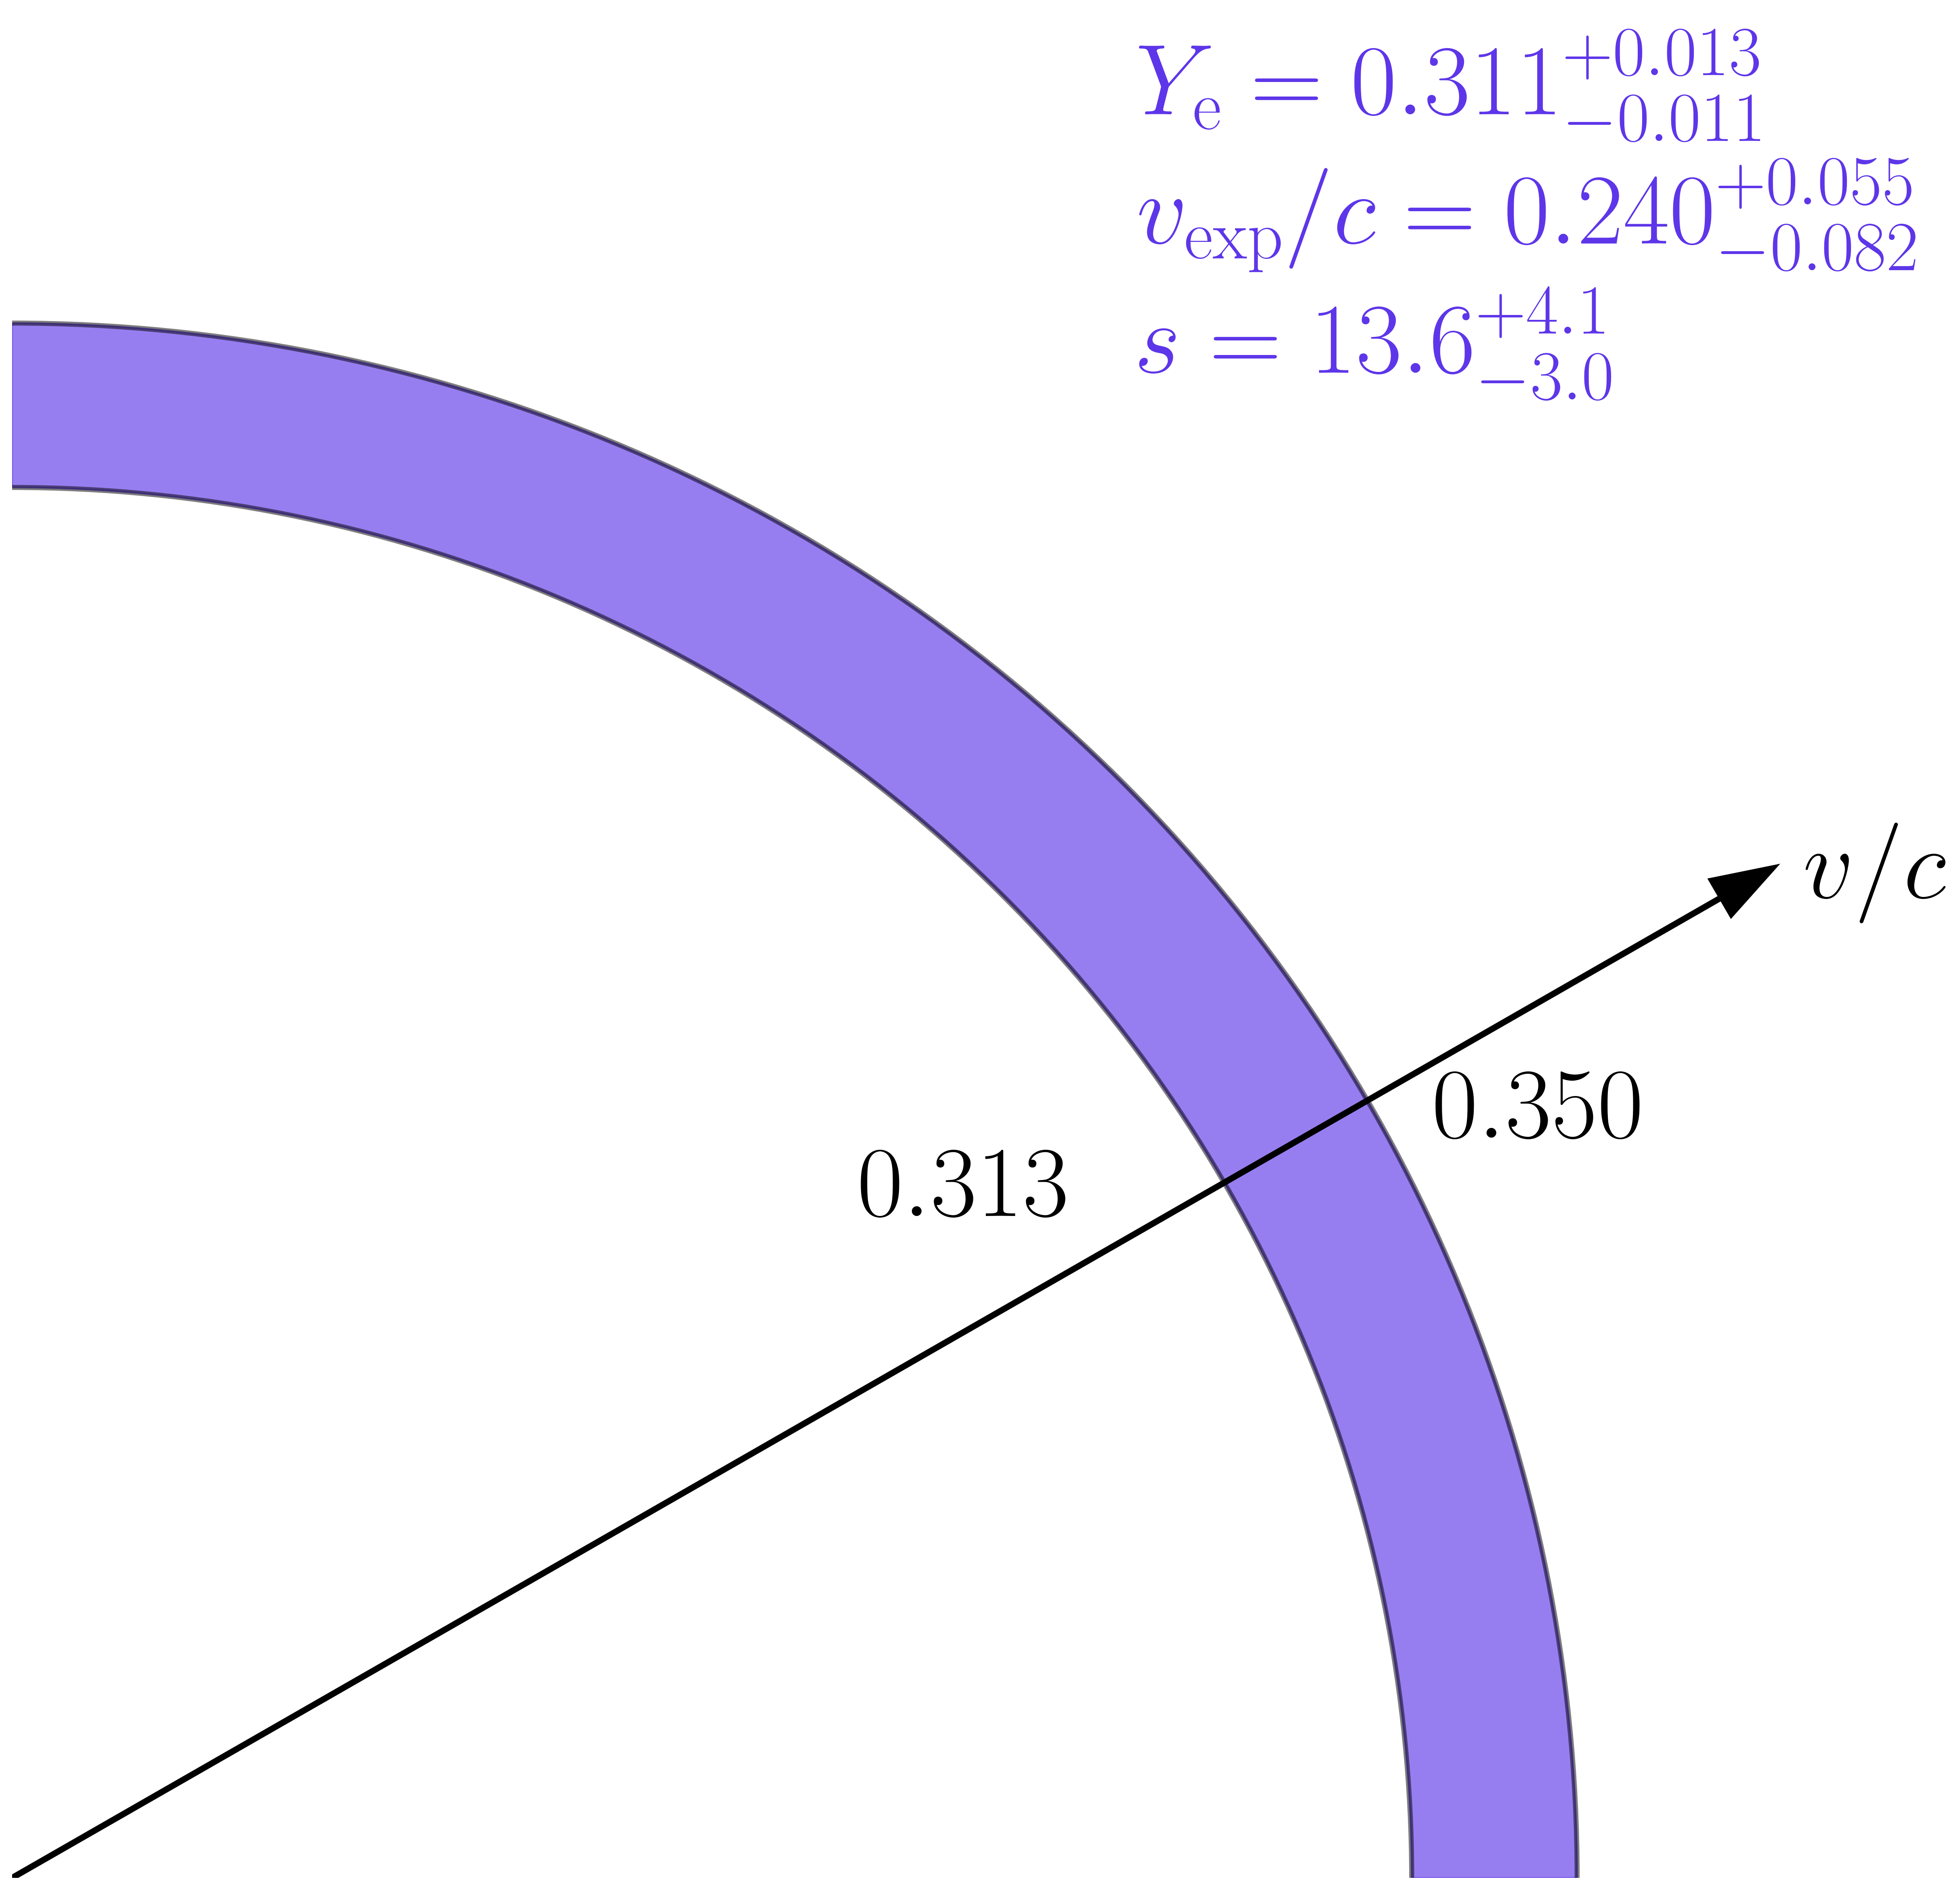
\includegraphics[width=0.47\textwidth]{figs/wedge_example_purplewarm.png}
%     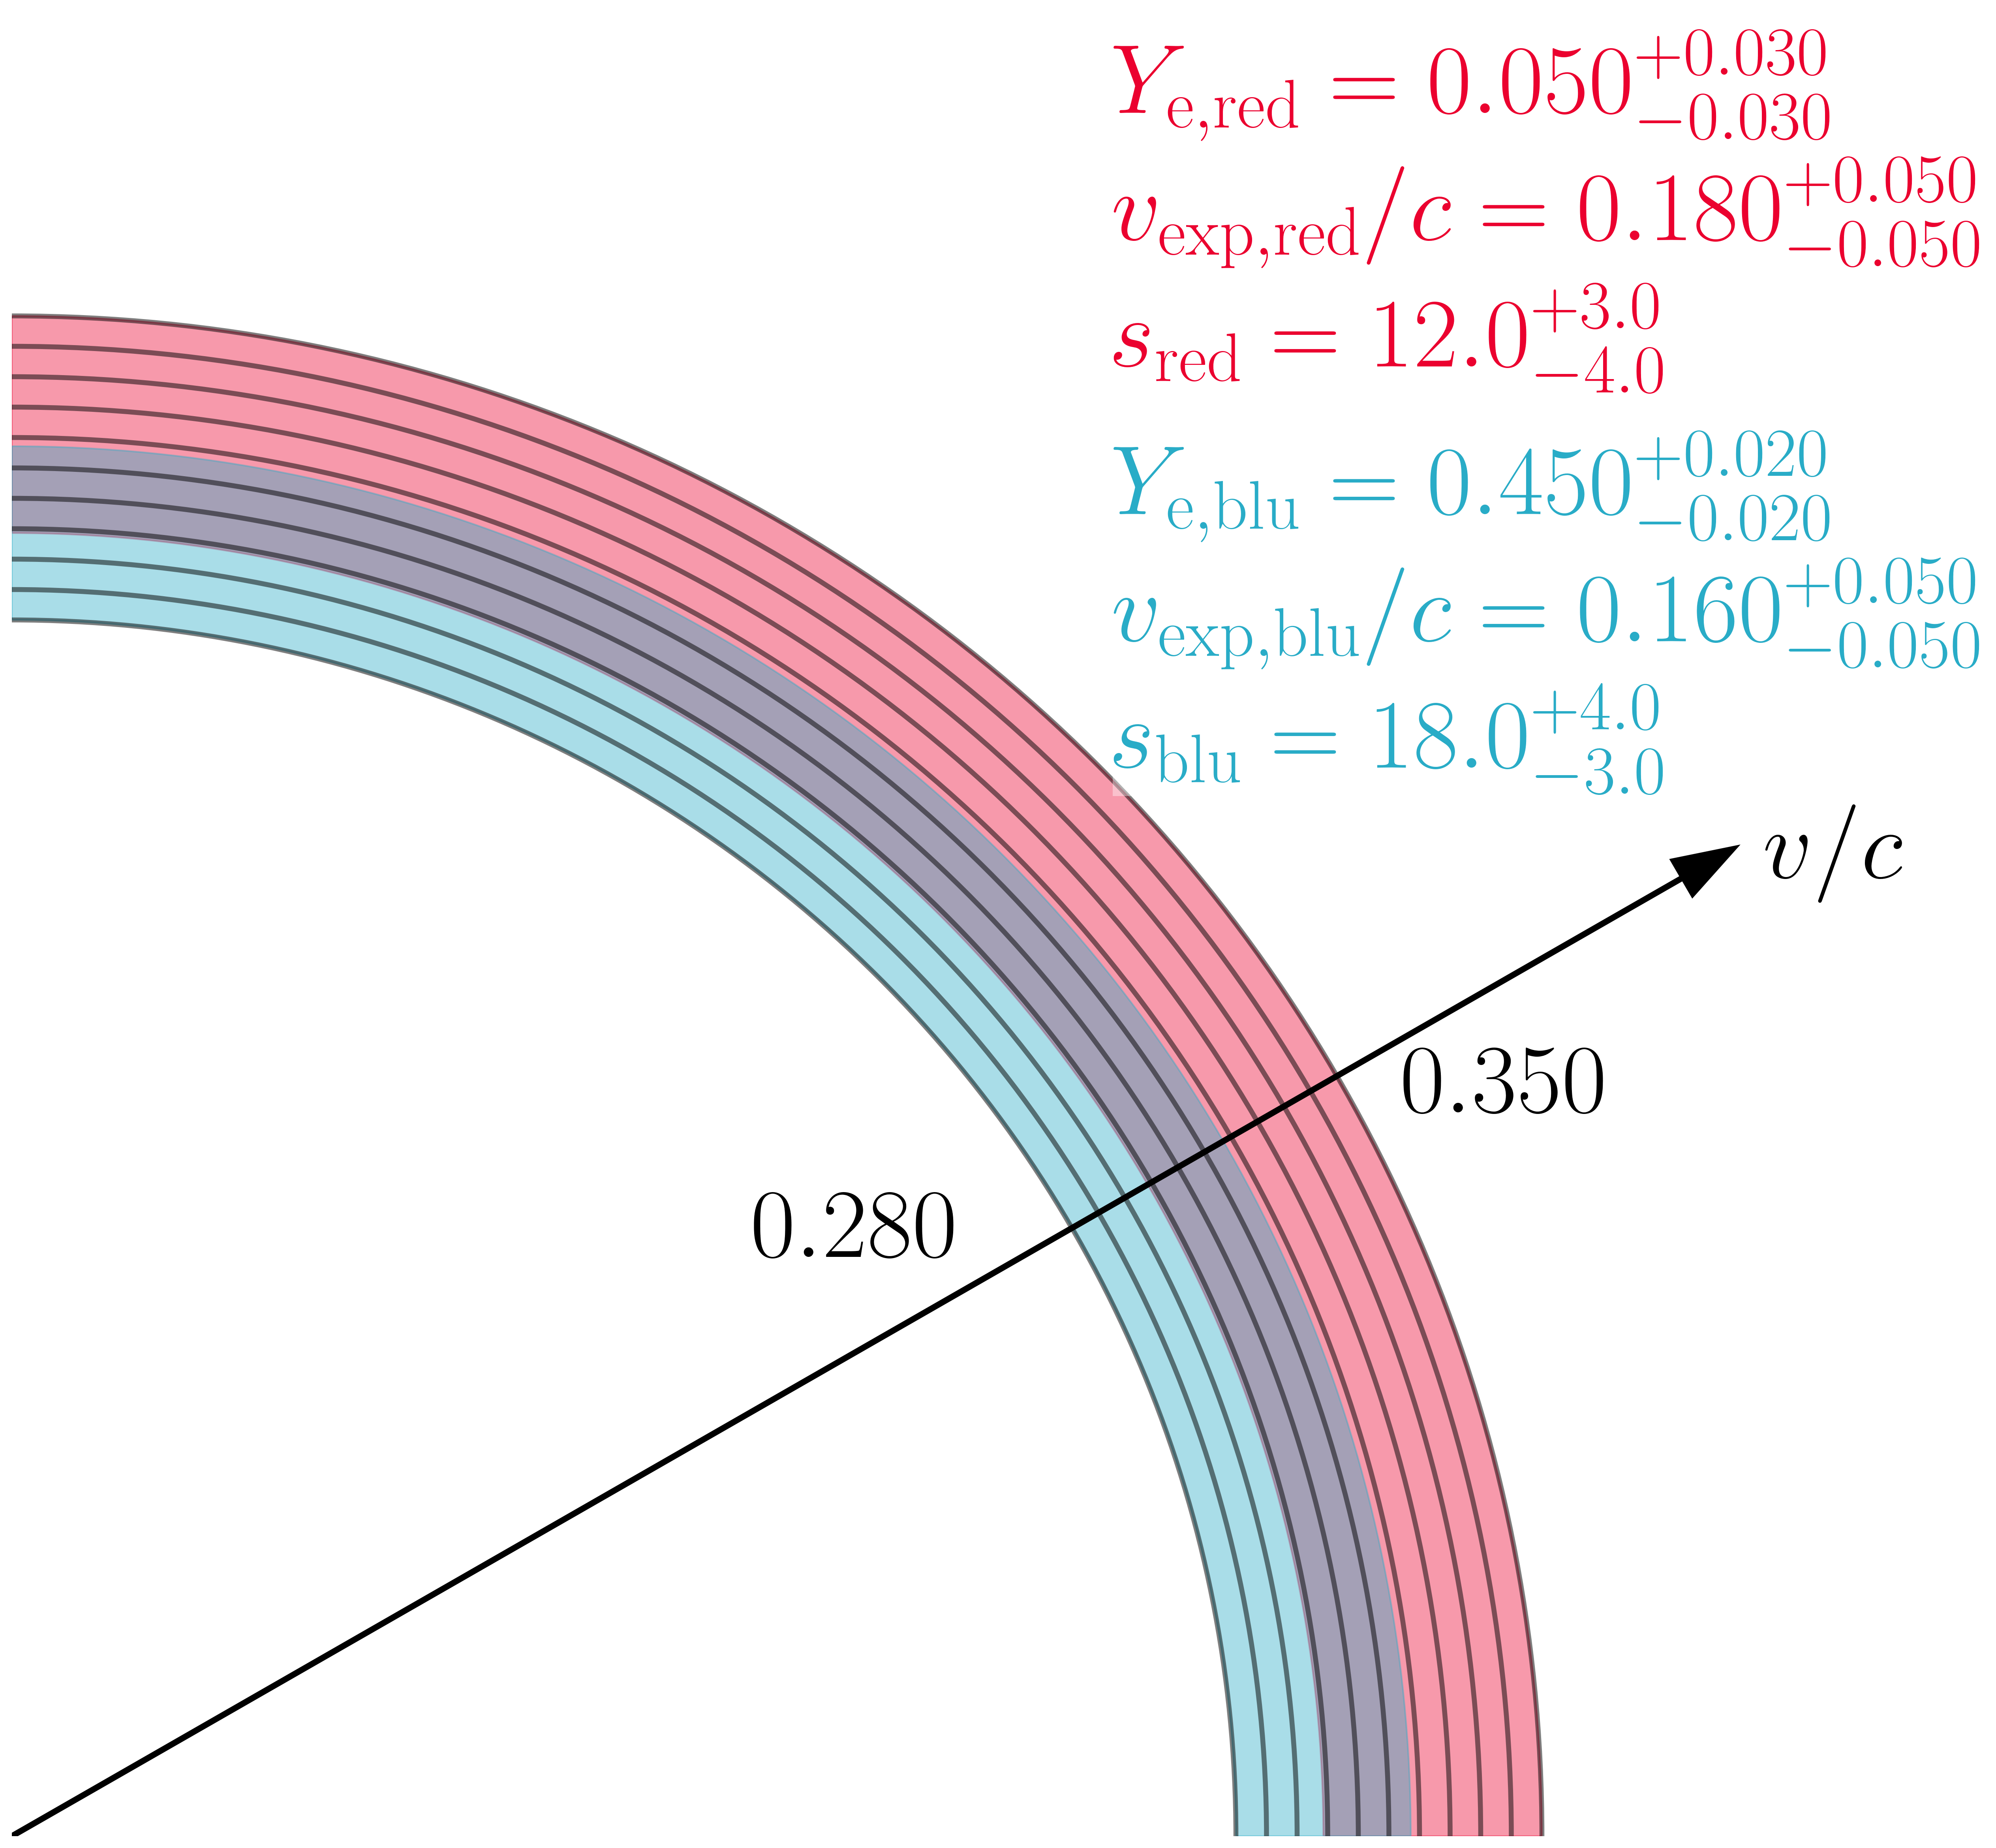
\includegraphics[width=0.47\textwidth]{figs/wedge_example_multicomp_redblu.png}
%     \figcaption{\textbf{Illustration of the difference between our single- and multi-component models.} \textit{Top:} A single-component ejecta, where the ejecta is not stratified and is characterized by a single $Y_e$, $v_{\mathrm{exp}}$, $s$, temperature, density, and other plasma properties. The abundance pattern is uniform in the one shell. The parameters shown here are those of the purple + warm model from V23. \textit{Bottom}: An example of multi-component ejecta, where the ejecta is stratified over 10 radial shells. A ``blue'' and ``red'' component are shown. The shells which span only the blue component have their abundance set by $Y_{e,2}$, $v_{\mathrm{exp,2}}$, and $s_{2}$, and the red by the equivalent parameters for the red component. Where components overlap, the abundances are summed and re-normalized to sum to unity. In this physical setup, the larger amount of lanthanides in the red component might lead to ``lanthanide curtaining'', where the emission from the blue component is re-processed by the red component and an overall redder kilonova is produced. }\label{fig:wedge_examples}
% \end{figure}


In V23, we model the kilonova ejecta as a single shell with a uniform abundance pattern. The plasma in this shell is also described by a single temperature and mass/electron density. This configuration is fully described by: the luminosity at the outer boundary $L_{\mathrm{outer}}$, (which in fact sets the initial guess for the temperature at the inner boundary), the normalization in the density power law $\rho_0$, the inner and outer boundary velocities $v_{\mathrm{inner}}$ and $v_{\mathrm{outer}}$, and three parameters which set the abundances: electron fraction $Y_e$, expansion velocity $v_{\mathrm{exp}}$, and specific entropy $s / k_{\mathrm{B}}$. A single-component fit is thus 7-dimensional, unless one or more of the parameters are fixed, \eg, we fix $v_{\mathrm{outer}} = 0.35c$ in our fit to the 1.4 day spectrum. This setup can describe a single ejecta component such as the tidal ejecta mostly confined to the equatorial plane, an outflow from a remnant accretion disk, or the squeezed polar ejecta from the collision interface during the merger. It may also describe a kilonova in which one component significantly dominates (by mass or by the strength of the absorption/emission features) over the other(s). 
    
Here, we implement multi-component, stratified ejecta. \TARDIS~allows for ejecta composed of stratified radial shells, each with a specific temperature, density, plasma conditions, and composition. In this configuration, each shell can have a specific abundance pattern. We use 10 shells in all runs unless indicated otherwise. We also employ multiple (30) \TARDIS~iterations when generating synthetic spectra in this configuration. At each iteration, the plasma conditions are updated, and converge towards an ejecta where the outer boundary emitted luminosity matches the user-requested $L_{\mathrm{outer}}$. 
    
We begin with a simple two-component ejecta. As with our single-component model, this two-component model is described by an outer boundary luminosity $L_{\mathrm{outer}}$ and $\rho_0$. Each of the components is then described by inner and outer boundary $v_{\mathrm{inner}}$ and $v_{\mathrm{outer}}$ and a $Y_e$, $v_{\mathrm{exp}}$, and $s / k_{\mathrm{B}}$. Multi-component fits are thus $2 + 5 + 5 = 12$-dimensional. The components necessarily overlap in physical space because \TARDIS~cannot simulate a gap between them. The abundance in each shell is then determined by the component(s) which are in a given shell. For shells where there is overlap between two components, the abundance is taken as a sum of the two abundance patterns and re-normalized to unity. %We graphically show the difference between single- and multi-component ejecta in Figure~\ref{fig:wedge_examples}.
    
Multiple components allow for additional complexity in the spectral synthesis.\footnote{See \cite{kawaguchi20} for an exploration of the diversity of kilonovae which may be produced when multiple components are present.} In particular, even in 1D with \TARDIS, we can produce the effect of re-processing, where emission from one component is absorbed and reemitted/scattered by another. We can also produce the effect of ``lanthanide curtaining'', in which some outermost lower-$Y_e$ ejecta containing the lanthanides masks an inner, bluer, lighter-element ejecta due to the considerable opacity of the lanthanides in the near-UV and optical. Some kilonova spectra may be better-described by these multi-component ejecta models. In V23, we find that the 1.4 day spectrum of the GW170817 kilonova is well-described by a single-component ejecta with $Y_e \sim 0.3-0.35$. However, at later epochs, as the ejecta expands and becomes more optically thin, the photosphere recedes into the ejecta and we may unmask additional components which were hidden at early times. Light curve modelling (\eg, \citealt{villar17}) has shown that the kilonova may indeed be better-described by multiple components of different opacities, and some spectral modelling (\eg, \citealt{kasen17}) also invokes multiple components. This motivates our introduction of multi-component ejecta into \SPARK. We fit the 1.4, 2.4, and 3.4 day spectra of the GW170817 kilonova with both single- and multi-component models to assess the need for multiple components.

% \begin{itemize}

%     \item In V23, we model the kilonova ejecta as a single shell with a uniform abundance pattern. The plasma in this shell is also described by a single temperature and mass/electron density. This configuration is fully described by the luminosity at the outer boundary $L_{\mathrm{outer}}$, (which in fact sets the temperature at the inner boundary), the normalization in the density power law $\rho_0$, the inner and outer boundary velocities $v_{\mathrm{inner}}$ and $v_{\mathrm{outer}}$, and three parameters which set the abundances: electron fraction $Y_e$, expansion velocity $v_{\mathrm{exp}}$, and specific entropy $s / k_{\mathrm{B}}$. A single-component fit is thus 7-dimensional, unless one or more of the parameters are fixed, \eg, we fix $v_{\mathrm{outer}} = 0.35c$ in our fit to the 1.4 day spectrum. This setup can describe a single ejecta component, \eg, the tidal ejecta mostly confined to the equatorial plane, an outflow from a remnant accretion disk, or the squeezed polar ejecta from the collision interface during the merger. It may also describe a kilonova in which one component significantly dominates (by mass or by the strength of the absorption/emission features) over the other(s). 
    
%     \item Here, we implement multi-component, stratified ejecta. \TARDIS~allows for ejecta composed of stratified shells, each with a specific temperature, density, and plasma conditions. In this configuration, each shell can have a specific abundance pattern. We use 10 shells in all runs unless indicated otherwise. We also employ multiple (30) \TARDIS~iterations when generating synthetic spectra in this configuration. At each iteration, the plasma conditions are updated, and converge towards an ejecta where the outer boundary emitted luminosity matches the user-requested $L_{\mathrm{outer}}$. 
    
%     \item We begin with a simple two-component ejecta. As with our single-component model, this two-component model is described by an outer boundary luminosity $L_{\mathrm{outer}}$ and $\rho_0$. Each of the components is then described by inner and outer boundary $v_{\mathrm{inner}}$ and $v_{\mathrm{outer}}$ and a $Y_e$, $v_{\mathrm{exp}}$, and $s / k_{\mathrm{B}}$. Multi-component fits are thus $2 + 5 + 5 = 12$-dimensional. The components necessarily overlap in physical space because \TARDIS~cannot simulate a gap between them. The abundance in each shell is then determined by the component(s) which are in a given shell. For shells where there is overlap between two components, the abundance is taken as a sum of the two abundance patterns. We graphically show the difference between single- and multi-component ejecta in \redbf{Figure X}.
    
%     \item Multiple components allow for additional complexity in the spectral synthesis.\footnote{See \cite{kawaguchi20} for a description of the diversity of kilonovae which may be produced when multiple components are present.} In particular, even in 1D with \TARDIS, we can produce the effect of re-processing, where emission from one component is absorbed and reemitted/scattered by another. We can also produce the effect of ``lanthanide curtaining'', in which some outermost lower-$Y_e$ ejecta containing the lanthanides masks an inner, bluer, lighter-element ejecta due to the considerable opacity of the lanthanides in the near-UV and optical. Some kilonova spectra may be better-described by these multi-component ejecta models. In V23, we find that the 1.4 day spectrum of the GW170817 kilonova is well-described by a single-component ejecta with $Y_e \sim 0.3$. However, at later epochs, as the ejecta expands and becomes more optically thin, the photosphere recedes into the ejecta and we may unmask additional components which were hidden at early times. Light curve modelling (\eg, \citealt{villar17}) has shown that the kilonova may indeed be better-described by multiple components of different opacities, and some spectral modelling (\eg, \citealt{kasen17}) also invokes multiple components. This motivates our introduction of multi-component ejecta into \SPARK. We fit the 1.4, 2.4, and 3.4 day spectra of the GW170817 kilonova with both single- and multi-component models to assess the need for multiple components.

% \end{itemize}



%%% SUBSECTION 2.3
\subsection{Inference setup}\label{ssc:inference-setup}

All \texttt{approxposterior}/BAPE hyperparameters and optimizers used here are the same as those used in V23. We again produce a baseline run of $m_{0} = 1500$ Latin Hypercube sampled points at the beginning of each \SPARK~run. However, the parameter space allowed by our priors differs for the 1.4, 2.4, and 3.4 day fits. Table~\ref{tab:priors-single} includes our priors for each of our single-component fits. All priors are uniform. The bounds on the density $\rho_0$ and abundance-setting parameters $Y_e$, $v_{\mathrm{exp}}$, and $s$ are the same at all epochs. The priors differ in the bounds on the luminosity, as expected given the cooling of the ejecta over time as it expands. We further allow for wider priors on the inner and outer boundary velocities for the fits at later epochs. In V23, we fixed $v_{\mathrm{outer}} = 0.35c$ during our 1.4 day fit but noted that we observed similar results for $v_{\mathrm{outer}}$ in the range $0.35 - 0.38c$. Here, we allow for greater flexibility in our fits to the later epochs.
    
Our priors for our multi-component fits are given in Table~\ref{tab:priors-multi}. These are identical at all epochs. The priors for the two components in a given fit are also identical, except that one of the components (`component 2') cannot extend as deep into the ejecta as the other (`component 1'). Our priors also ensure some overlap between the two components. % To allow for even sampling of parameter space for the $m_0 = 1500$ points in the base training set with this complex conditional prior, we use constrained Latin Hypercube Sampling (cLHS; \citealt{petelet09}).
    
When attempting to fit the 3.4 day spectrum, we find that the fit converges to a blackbody with little to no absorption in order to fit the continuum of the spectrum, especially at the shortest wavelengths. Since we are interested in determining the species involved in the absorption, and the employed observed line list is likely especially incomplete at the shortest wavelengths, we prioritize fitting the $\geqslant 6400$~\AA~region of the spectrum. We exclude wavelengths shorter than $6400$~\AA~when fitting the spectrum at 3.4 days, for both single- and multi-component fits.

Finally, when writing down the likelihood using the \cite{czekala15} formalism, we use a global covariance term with amplitude $a_{\mathrm{G}} = 10^{-34}~(\mathrm{erg~s^{-1}~cm^{-2}}$~\text{\AA}${}^{-1})^{2}$ and a correlation length scale $\ell = 0.025c$ for all 1.4 and 2.4 day fits. For 3.4 day fits, after some trial and error, we find that a smaller $a_{\mathrm{G}} = 10^{-35}~(\mathrm{erg~s^{-1}~cm^{-2}}$~\text{\AA}${}^{-1})^{2}$ better captures the overall smaller uncertainties on the observed spectrum, as the spectrum has faded by this time.




\begin{deluxetable}{c|ccc}
\centering
\tablecaption{Uniform priors for the parameters of the single-component fits at 1.4, 2.4, and 3.4 days. $v_{\mathrm{outer}}$ is fixed to $0.35c$ in the 1.4 day fit (V23).}
\tablehead{parameter & 1.4 days & 2.4 days & 3.4 days}
\startdata\tablewidth{1.0\textwidth}
 \vspace{2pt}
$\log_{10}(L_\mathrm{outer}/L_{\odot})$ & $[7.6, 8.0]$ & $[7.2, 7.8]$ & $[7.2, 7.8]$ \\ 
$\log_{10}(\rho_0/\mathrm{g~cm^{-3}})$ & $[-16.0, -14.0]$ & same & same \\
$v_{\mathrm{inner}}/c$& $[0.250, 0.340]$ & $[0.100, 0.275]$ & $[0.100, 0.275]$ \\
$v_{\mathrm{outer}}/c$& - & $[0.280, 0.400]$ & $[0.280, 0.400]$ \\
$v_{\mathrm{exp}}/c$ & $[0.05, 0.30]$ & same & same \\
$Y_e$ & $[0.01, 0.40]$ & same & same \\
$s~[k_{\mathrm{B}}/\mathrm{nucleon}]$ & $[10, 35]$ & same & same \\
\enddata
\end{deluxetable}\label{tab:priors-single}


\begin{deluxetable}{c|c}
\centering
\tablecaption{Uniform priors for the parameters of the multi-component fits at 1.4, 2.4, and 3.4 days.}
\tablehead{parameter & prior}
\startdata\tablewidth{1.0\textwidth}
 \vspace{2pt}
$\log_{10}(L_\mathrm{outer}/L_{\odot})$ & $[7.0, 8.0]$ \\ 
$\log_{10}(\rho_0/\mathrm{g~cm^{-3}})$ & $[-16.0, -14.0]$ \\\hline
$v_{\mathrm{inner,1}}/c$& $[0.10, 0.29]$ \\
$v_{\mathrm{outer,1}}/c$ &  $[0.30, 0.40]$ \\
$v_{\mathrm{exp,1}}/c$ & $[0.05, 0.30]$ \\
$Y_{e,1}$ & $[0.01, 0.50]$ \\
$s_{1}~[k_{\mathrm{B}}/\mathrm{nucleon}]$ & $[10, 35]$ \\\hline
$v_{\mathrm{inner,2}}/c$& $[0.20, 0.31]$ \\
$v_{\mathrm{outer,2}}/c$ &  $[0.31, 0.40]$ \\
$v_{\mathrm{exp,2}}/c$ & $[0.05, 0.30]$ \\
$Y_{e,2}$ & $[0.01, 0.50]$ \\
$s_{2}~[k_{\mathrm{B}}/\mathrm{nucleon}]$ & $[10, 35]$ \\
\enddata
\end{deluxetable}\label{tab:priors-multi}


%%% === SECTION 3 === %%%
%% RESULTS %%

\section{Results}\label{sec:results}

\begin{deluxetable}{cccc}
\centering
\tablecaption{Best-fit parameters for single-component fits to the GW170817 kilonova at $1.4$, $2.4$, and $3.4$~days. The $1.4$~day fit is the ``purple + warm'' model of V23. $v_{\mathrm{outer}}$ is fixed to $0.35c$ in the 1.4 day fit. The inner boundary temperature $T_{\mathrm{inner}}$ and lanthanide mass fraction $X_{\mathrm{lan}}$ are derived parameters, \ie, they are not dimensions in $\theta$-space.}
\tablehead{parameter & 1.4 days & 2.4 days & 3.4 days}
\startdata\tablewidth{1.0\textwidth}
 \vspace{2pt}
$\log_{10}(\frac{L_\mathrm{outer}}{L_{\odot}})$ & $7.782^{+0.013}_{-0.014}$ & $7.594^{+0.040}_{-0.061}$ & $7.531^{+0.017}_{-0.016}$ \\ 
$\log_{10}(\frac{\rho_0}{\mathrm{g~cm^{-3}}})$ & $-15.016^{+0.320}_{-0.316}$ & $-15.443^{+0.742}_{-0.463}$ & $-14.586^{+0.313}_{-0.384}$ \\ 
$v_{\mathrm{inner}}/c$ & $0.313^{+0.013}_{-0.014}$ & $0.249^{+0.017}_{-0.032}$ & $0.253^{+0.011}_{-0.021}$ \\
$v_{\mathrm{outer}}/c$ & $0.35$ & $0.342^{+0.047}_{-0.050}$  & $0.309^{+0.032}_{-0.023}$ \\
$v_{\mathrm{exp}}/c$ & $0.240^{+0.055}_{-0.082}$ & $0.172^{+0.107}_{-0.101}$ & $0.132^{+0.094}_{-0.056}$ \\
$Y_e$ & $0.311^{+0.013}_{-0.011}$ & $0.306^{+0.055}_{-0.204}$ & $0.226^{+0.062}_{-0.067}$ \\
$s~[k_{\mathrm{B}}/\mathrm{nuc}]$ & $13.6^{+4.1}_{-3.0}$ & $17.6^{+7.1}_{-6.3}$ & $15.4^{+7.1}_{-6.3}$ \\ \hline
$T_{\mathrm{inner}}~[\mathrm{K}]$ & $3958^{+87}_{-94}$ & $3050^{+126}_{-223}$ & $2455^{+59}_{-104}$ \\ 
%$X_{\mathrm{lan}}$ & $1.8^{+26.3}_{-1.8}\times 10^{-7}$ & $9.5^{+355.1}_{-6.6}\times 10^{-8} $ & $\sim1.1\times 10^{-2}$\\
$\log_{10} X_{\mathrm{lan}}$ & ${-7.03}^{+0.46}_{-0.47}$ & $-5.64^{+1.05}_{-1.31}$ & $-2.10^{+1.28}_{-6.20}$ \\
\enddata
\end{deluxetable}\label{tab:bestfit_single}

%% compilation of all fits; Fig. 1
\begin{figure*}[!ht]
    \centering
    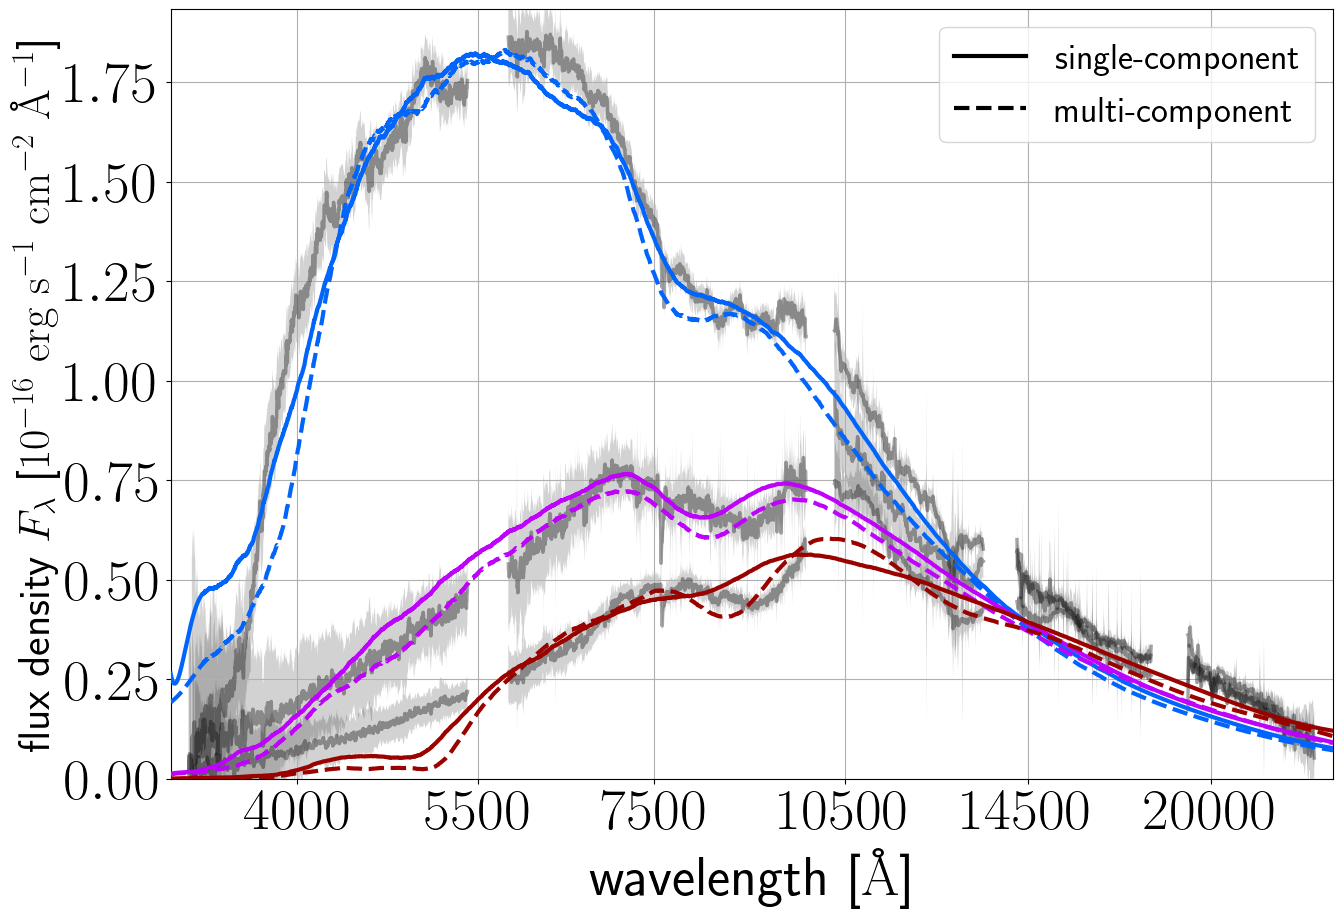
\includegraphics[width=0.98\textwidth]{figs/bestfits_compare_all_SPARK_2.png}
    \figcaption{\textbf{Compilation of all best-fit models to the spectrum of the GW170817 kilonova, AT2017gfo, from this work: 1.4, 2.4, and 3.4 days post-merger, for both single- and multi-component models.} The single-component models are favored at 1.4 and 2.4 days. At 3.4 days, we require a multi-component ejecta to adequately fit the spectrum. The abundance patterns corresponding to these preferred models are included in Figure~\ref{fig:abunds_time_evolution}. All best fits are obtained as the median of the posterior, or the median of some mode of the posterior. The full posteriors are included in Appendices~\ref{app:corners_single}~and~\ref{app:corners_multi} for single- and multi-component models, respectively.}\label{fig:bestfits}
\end{figure*}


In Figure~\ref{fig:bestfits}, we compile our best-fit spectra for the GW170817 kilonova at 1.4, 2.4, and 3.4 days, for both single- and multi-component models. In the following sections, we present and examine each of the best fits in turn. We assess the convergence of the GP surrogate, and the posterior, in Appendix~\ref{app:convergence}.


%%% subsection: SINGLE-COMPONENT 2.4 AND 3.4 DAY FITS
\subsection{Single-component fits at 2.4 and 3.4 days}\label{ssc:2.4_3.4_fits}

Appendix~\ref{app:allspec_single} contains compilations of all $m_0 + m_{\mathrm{active}}$ spectra generated in a given \SPARK~run, for the 2.4 day and 3.4 day single-component fits. The posteriors generated by these \SPARK~runs are included in Appendix~\ref{app:corners_single}. Unless stated otherwise, we use the median of the posterior, or the median of some mode of a multi-modal posterior, to determine our best fit and uncertainties. The best-fit parameters for 1.4 days, single-component (V23) and 2.4, 3.4 days, single-component (this work) are given in Table~\ref{tab:bestfit_single}. We examine the 2.4 and 3.4 day models below.


%%% subsubsection: 2.4 DAYS, SINGLE-COMPONENT
\subsubsection{Single-component, 2.4 days}\label{sssc:2.4_single}

We require $m_0 + m_{\mathrm{active}} = 1500 + 600$ points to obtain a good fit and converged posterior in our 2.4 day, single-component \SPARK~run. Interestingly, the resultant posterior shows some bimodality, most evident in the $s/k_{\mathrm{B}}$ dimension. Discarding samples from the posterior with $s/k_{\mathrm{B}} \geqslant 25.0$, we obtain our preferred fit. This fit captures most of the continuum of the observed spectrum, and most of the $\sim8000$~\AA~absorption. If this absorption indeed belongs to a P Cygni feature, we do partially miss the longer-wavelength ``wing'' of this feature. Furthermore, we overestimate the absorption, or underestimate the continuum, at the shortest wavelengths. 

We infer an outer boundary luminosity of $\log_{10} (L_{\mathrm{outer}}/L_{\odot}) = 7.594^{+0.040}_{-0.061}$, or equivalently, $L_{\mathrm{outer}} = $. In the case of single-shell, single-\TARDIS~iteration, we use these values to determine an inner boundary temperature of $T_{\mathrm{inner}} = 3050^{+126}_{-223}~\mathrm{K}$. As expected, the kilonova has dimmed and cooled since the previous epoch at 1.4 days. Inferring the structure of the ejecta, we find $\log_{10} (\rho_0 / \mathrm{g~cm^{-3}}) = -15.443^{+0.742}_{-0.463}$, or equivalently $\rho_0 = $. We also obtain the inner and outer boundary velocities, $v_{\mathrm{inner}}/c = 0.249^{+0.017}_{-0.032}$ and $v_{\mathrm{outer}} = 0.342^{+0.047}_{-0.050}$. This $v_{\mathrm{outer}}$ is consistent with the fixed $v_{\mathrm{outer}} = 0.35c$ from 1.4 days. In contrast, $v_{\mathrm{inner}}$---effectively the photospheric velocity---has receded into the ejecta. This is evidence for the ejecta expanding, cooling, and become optically thinner, as expected.  

Finally, we obtain an electron fraction $Y_e = 0.306^{+0.055}_{-0.204}$, expansion velocity $v_{\mathrm{exp}}/c = 0.172^{+0.107}_{-0.101}$, and specific entropy $s/k_{\mathrm{B}} = 17.6^{+7.1}_{-6.3}$. As at 1.4 days, $v_{\mathrm{exp}}$ is poorly constrained. $s$ is better-constrained, but is also consistent with the earlier epoch. The posterior distribution in all dimensions is wider at this epoch; in particular, $Y_e$ includes a tail extending to smaller electron fractions. The posterior is nonetheless peaked at $Y_e = 0.306^{+0.055}_{-0.204}$, which is slightly lower than at 1.4 days, but consistent within uncertainties. This can be seen in the lanthanide fraction: we find $\log_{10} X_{\mathrm{lan}} = -5.64^{+1.05}_{-1.31}$, too small to match the Solar $r$-process abundance pattern, as is the case at 1.4 days.

% \begin{itemize}
%     \item Point to the plot of all spectra in Figure~\ref{fig:all_spec_single} (Appendix~\ref{app:allspec_single}). $m_0 = 1500$ and $m_{\mathrm{active}} = 600$ samples. 

%     \item In the best fit, we overestimate the absorption at the shortest wavelengths. This is on contrast with 1.4 days, where we underestimated. We accurately model the absorption at 8000\AA, but miss the higher-wavelength bump, which is the red wing of a P-Cygni feature (in the P-Cygni interpretation). 

%     \item Point to the posterior. The full posterior is in Figure~\ref{fig:corner_single_2.4}. We find some bimodality, most evident in the $s/k_{\mathrm{B}}$ dimension. Discarding samples with $s/k_{\mathrm{B}} \geqslant 25.0$, we obtain our preferred model. This zoomed-in posterior is shown in Figure~\ref{fig:corner_single_2.4_zoom}.

%     \item Present $L_{\mathrm{outer}}$ and $T_{\mathrm{inner}}$. The kilonova has dimmed and the ejecta has cooled. 

%     \item Present the density and inner / outer boundary velocities. The photosphere has receded into the ejecta. The outer boundary velocity is consistent with $v_{\mathrm{outer}} = 0.35c$ fixed in the 1.4 day fit. Compute the total mass contained in the line-forming region of the ejecta? 

%     \item Highlight abundance-setting parameters: $Y_{\mathrm{e}}$, $v_{\mathrm{exp}}$, and $s$. $Y_{\mathrm{e}}$ is lower, but consistent with that inferred at 1.4 days. The expansion velocity and entropy are consistent with that of 1.4 days. In the posterior, $Y_{\mathrm{e}}$ has a tail which extends to lower electron fractions. The posterior in general is broader.

%     \item $X_{\mathrm{lan}}$ is smaller at 2.4 days, but still very lanthanide-poor. Inconsistent with Solar $r$-process.
    
% \end{itemize}


%%% subsubsection: 3.4 DAYS, SINGLE-COMPONENT
\subsubsection{Single-component, 3.4 days}\label{sssc:3.4_single}

Our best single-component model for 3.4 days is in general a poor fit to the observed spectrum of AT2017gfo. Nonetheless, we review it here for completeness. The reader may skip to Section~\ref{sssc:3.4_multi} to see the preferred, multi-component model for this epoch. 

As at 2.4 days, we require $m_0 + m_{\mathrm{active}} = 1500 + 600$ points to obtain a converged posterior. The resultant posterior shows a high degree of multi-modality, most evident in the $\rho_0$, $Y_e$, and $s / k_{\mathrm{B}}$ dimensions. Of the multiple modes, we obtain our best (but still poor) fit to the observed spectrum by discarding samples from the posterior outside of the range $\log_{10}(\rho_0 / \mathrm{g~cm^{-3}}) \in [-15.0, -14.0] \cup Y_{\mathrm{e}} \in [0.13, 0.29] \cup s/k_{\mathrm{B}} \in [10.0, 25.0]$. This higher-$\rho_0$, mid-$Y_e$, low-$s$ mode produces some of the dominant absorption feature at $\sim8000$ \AA, but not all. This fit also overstimates the absorption or underestimates the continuum, for wavelengths $\lesssim 5500$ \AA. 

We infer an outer boundary luminosity of $\log_{10} (L_{\mathrm{outer}}/L_{\odot}) = 7.531^{+0.017}_{-0.016}$, or equivalently, $L_{\mathrm{outer}} = $. This luminosity corresponds to an inner boundary temperature $T_{\mathrm{inner}} = 2455^{+59}_{-104}~\mathrm{K}$. We find $\log_{10} (\rho_0 / \mathrm{g~cm^{-3}}) = -14.586^{+0.313}_{-0.384}$, or equivalently $\rho_0 = $. This density is inconsistent with (larger than) that inferred at earlier epochs, which may explain some of the poorness of the fit. We also obtain the inner and outer boundary velocities, $v_{\mathrm{inner}}/c = 0.253^{+0.032}_{-0.023}$ and $v_{\mathrm{outer}} = 0.309^{+0.032}_{-0.023}$. This $v_{\mathrm{outer}}$ is much smaller than is fixed at 1.4 days or inferred at 2.4 days. This may explain the insufficient absorption at $\sim8000$ \AA, if the photon packets are not interacting with enough matter to be absorbed in large numbers before escaping the ejecta.

Finally, we find an electron fraction $Y_e = 0.226^{+0.062}_{-0.067}$, expansion velocity $v_{\mathrm{exp}}/c = 0.132^{+0.094}_{-0.056}$, and specific entropy $s/k_{\mathrm{B}} = 15.4^{+7.2}_{-3.1}$ at this epoch. $v_{\mathrm{exp}}$ is once again poorly constrained, and $s$ is once again consistent with earlier epochs. In contrast, $Y_e$ is lower and inconsistent with both previous epochs. Interestingly, despite the lower $Y_e$, the abundance of Sr---which has been identified as the source of the $\sim 8000$ \AA~absorption---is within a factor of $1$\% that of our single-component model at 1.4 days, and only $\sim 25$\% larger than that of our single-component model at 2.4 days. This suggests that the shortcomings of this model may be due to the differing densities and velocity structures, rather than the abundance-setting parameters.




%%% subsection: MULTI-COMPONENT 1.4, 2.4, AND 3.4 DAY FITS
\subsection{Multi-component fits at 1.4, 2.4, and 3.4 days}\label{ssc:1.4_2.4_3.4_multi_fits}


\begin{deluxetable*}{cccc}
\centering
\tablecaption{Best-fit parameters for multi-component fits to the GW170817 kilonova at $1.4$, $2.4$, and $3.4$~days. The ejecta mass in each component $M_{\mathrm{1; 2}}$, lanthanide mass fraction in each component $X_{\mathrm{lan,1; 2}}$, and the total $X_{\mathrm{lan,total}}$ are derived parameters, \ie, they are not dimensions in $\theta$-space.}
\tablehead{parameter & 1.4 days & 2.4 days & 3.4 days}
\startdata\tablewidth{1.0\textwidth}
 \vspace{2pt}
$\log_{10}(\frac{L_\mathrm{outer}}{L_{\odot}})$ & $7.853^{+0.014}_{-0.023}$ & $7.700^{+0.065}_{-0.073}$ & $7.605^{+0.049}_{-0.040}$ \\ 
$\log_{10}(\frac{\rho_0}{\mathrm{g~cm^{-3}}})$ & $-15.106^{+0.140}_{-0.586}$ & $-15.440^{+0.813}_{-0.467}$ & $-14.505^{+0.323}_{-0.372}$ \\ \hline
$v_{\mathrm{inner,1}}/c$ & $0.322^{+0.007}_{-0.031}$ & $0.260^{+0.061}_{-0.039}$ & $0.213^{+0.056}_{-0.035}$ \\
$v_{\mathrm{outer,1}}/c$ & $0.325^{+0.009}_{-0.016}$ & $0.335^{+0.054}_{-0.065}$ & $0.344^{+0.035}_{-0.038}$ \\
$v_{\mathrm{exp,1}}/c$ & $0.120^{+0.027}_{-0.026}$ & $0.170^{+0.108}_{-0.100}$ & $0.198^{+0.092}_{-0.102}$ \\
$Y_{e,1}$ & $0.133^{+0.033}_{-0.120}$ & $0.288^{+0.129}_{-0.187}$ & $0.228^{+0.073}_{-0.088}$ \\
$s_{1}~[k_{\mathrm{B}}/\mathrm{nuc}]$ & $24.4^{+3.6}_{-5.3}$ & $21.1^{+10.5}_{-9.5}$ & $14.9^{+8.0}_{-4.5}$ \\ \hline
$v_{\mathrm{inner,2}}/c$ & $0.281^{+0.012}_{-0.017}$ & $0.268^{+0.049}_{-0.045}$ & $0.232^{+0.038}_{-0.027}$ \\
$v_{\mathrm{outer,2}}/c$ & $0.356^{+0.015}_{-0.015}$ & $0.335^{+0.045}_{-0.070}$ & $0.334^{+0.037}_{-0.022}$ \\
$v_{\mathrm{exp,2}}/c$ & $0.193^{+0.036}_{-0.037}$ & $0.183^{+0.089}_{-0.110}$ & $0.134^{+0.091}_{-0.069}$ \\
$Y_{e,2}$ & $0.338^{+0.021}_{-0.021}$ & $0.261^{+0.163}_{-0.124}$ & $0.161^{+0.149}_{-0.104}$ \\
$s_{2}~[k_{\mathrm{B}}/\mathrm{nuc}]$ & $20.0^{+3.9}_{-3.5}$ & $22.0^{+10.0}_{-10.1}$ & $21.5^{+8.3}_{-9.5}$ \\ \hline\hline
$M_{1}~[M_{\odot}]$ & $2.7^{+0.9}_{-3.6}~\times 10^{-6}$ & $3.4^{+6.4}_{-3.7}\times 10^{-5}$ & $5.5^{+4.1}_{-4.8}~\times 10^{-4}$ \\
%$X_{\mathrm{lan,1}}$ & & $\sim1.1\times10^{-5}$ & $\geqslant 1.67 \times 10^{-2}$ \\ \hline
$\log_{10} X_{\mathrm{lan,1}}$ & $-1.16^{+0.38}_{-0.29}$ & $-0.63^{+0.26}_{-11.1}$ & $-0.97^{+0.29}_{-0.31}$ \\ \hline
$M_{2}~[M_{\odot}]$ & $6.9^{+2.2}_{-9.3}~\times 10^{-5}$ & $3.0^{+5.6}_{-3.3}\times 10^{-5}$ & $4.2^{+3.1}_{-3.6}~\times 10^{-4}$ \\
% $X_{\mathrm{lan,2}}$ & & $\sim2.4\times10^{-3}$ & $2.8^{+26.3}_{-1.1}\times10^{-2}$ \\ \hline
$\log_{10} X_{\mathrm{lan,2}}$ & $-12.99^{+2.98}_{-2.90}$ & $-4.53^{+2.61}_{-3.53}$ & $-0.88^{+0.32}_{-0.55}$ \\ \hline
$\log_{10} X_{\mathrm{lan,total}}$ & $-12.97^{+9.17}_{-2.37}$ & $-3.39^{+1.34}_{-1.75}$ & $-3.71^{+2.74}_{-4.40}$ \\
\enddata
\end{deluxetable*}\label{tab:bestfit_multi}


Appendix~\ref{app:allspec_multi} contains compilations of all $m_0 + m_{\mathrm{active}}$ spectra generated in a given \SPARK~run, for the 1.4, 2.4, and 3.4 day multi-component fits. The posteriors generated by these \SPARK~runs are included in Appendix~\ref{app:corners_multi}. The best-fit parameters for 1.4, 2.4, 3.4 days, multi-component are given in Table~\ref{tab:bestfit_multi}. We examine these new models below.


%% wedges; Fig 2
\begin{figure}[!ht]
    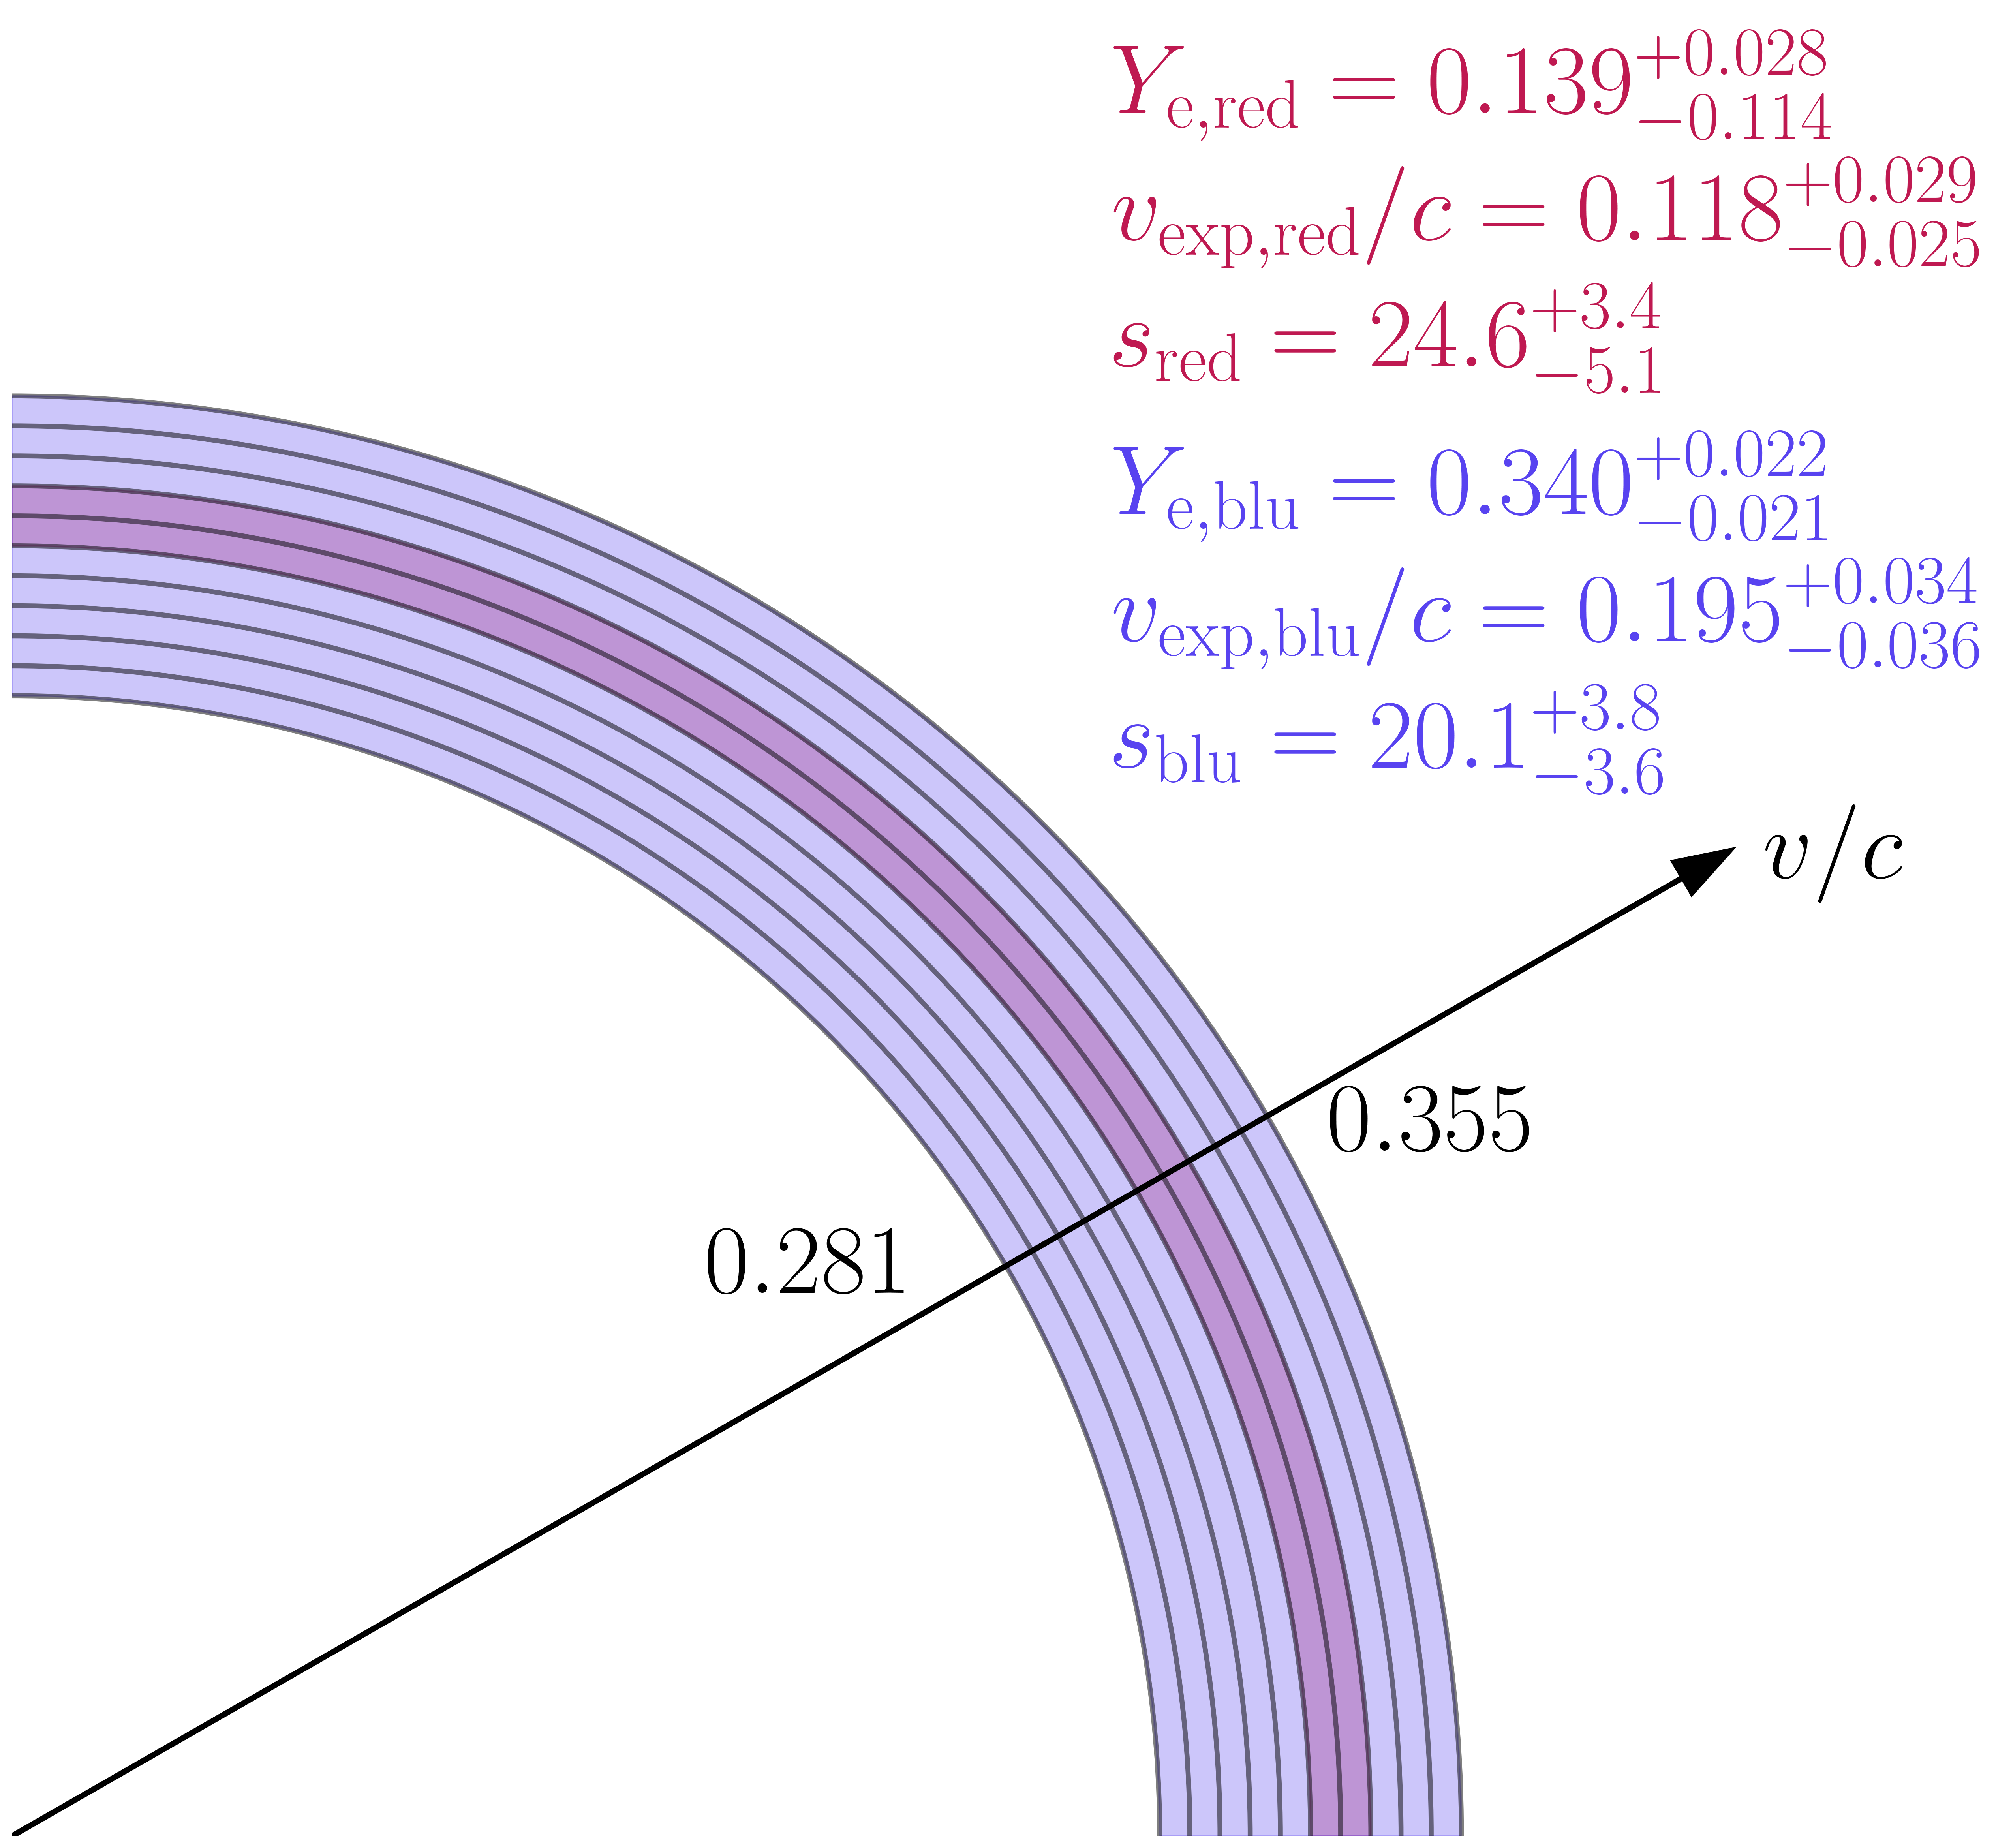
\includegraphics[width=0.4\textwidth]{figs/multicomp_wedges_1.4d.png}
    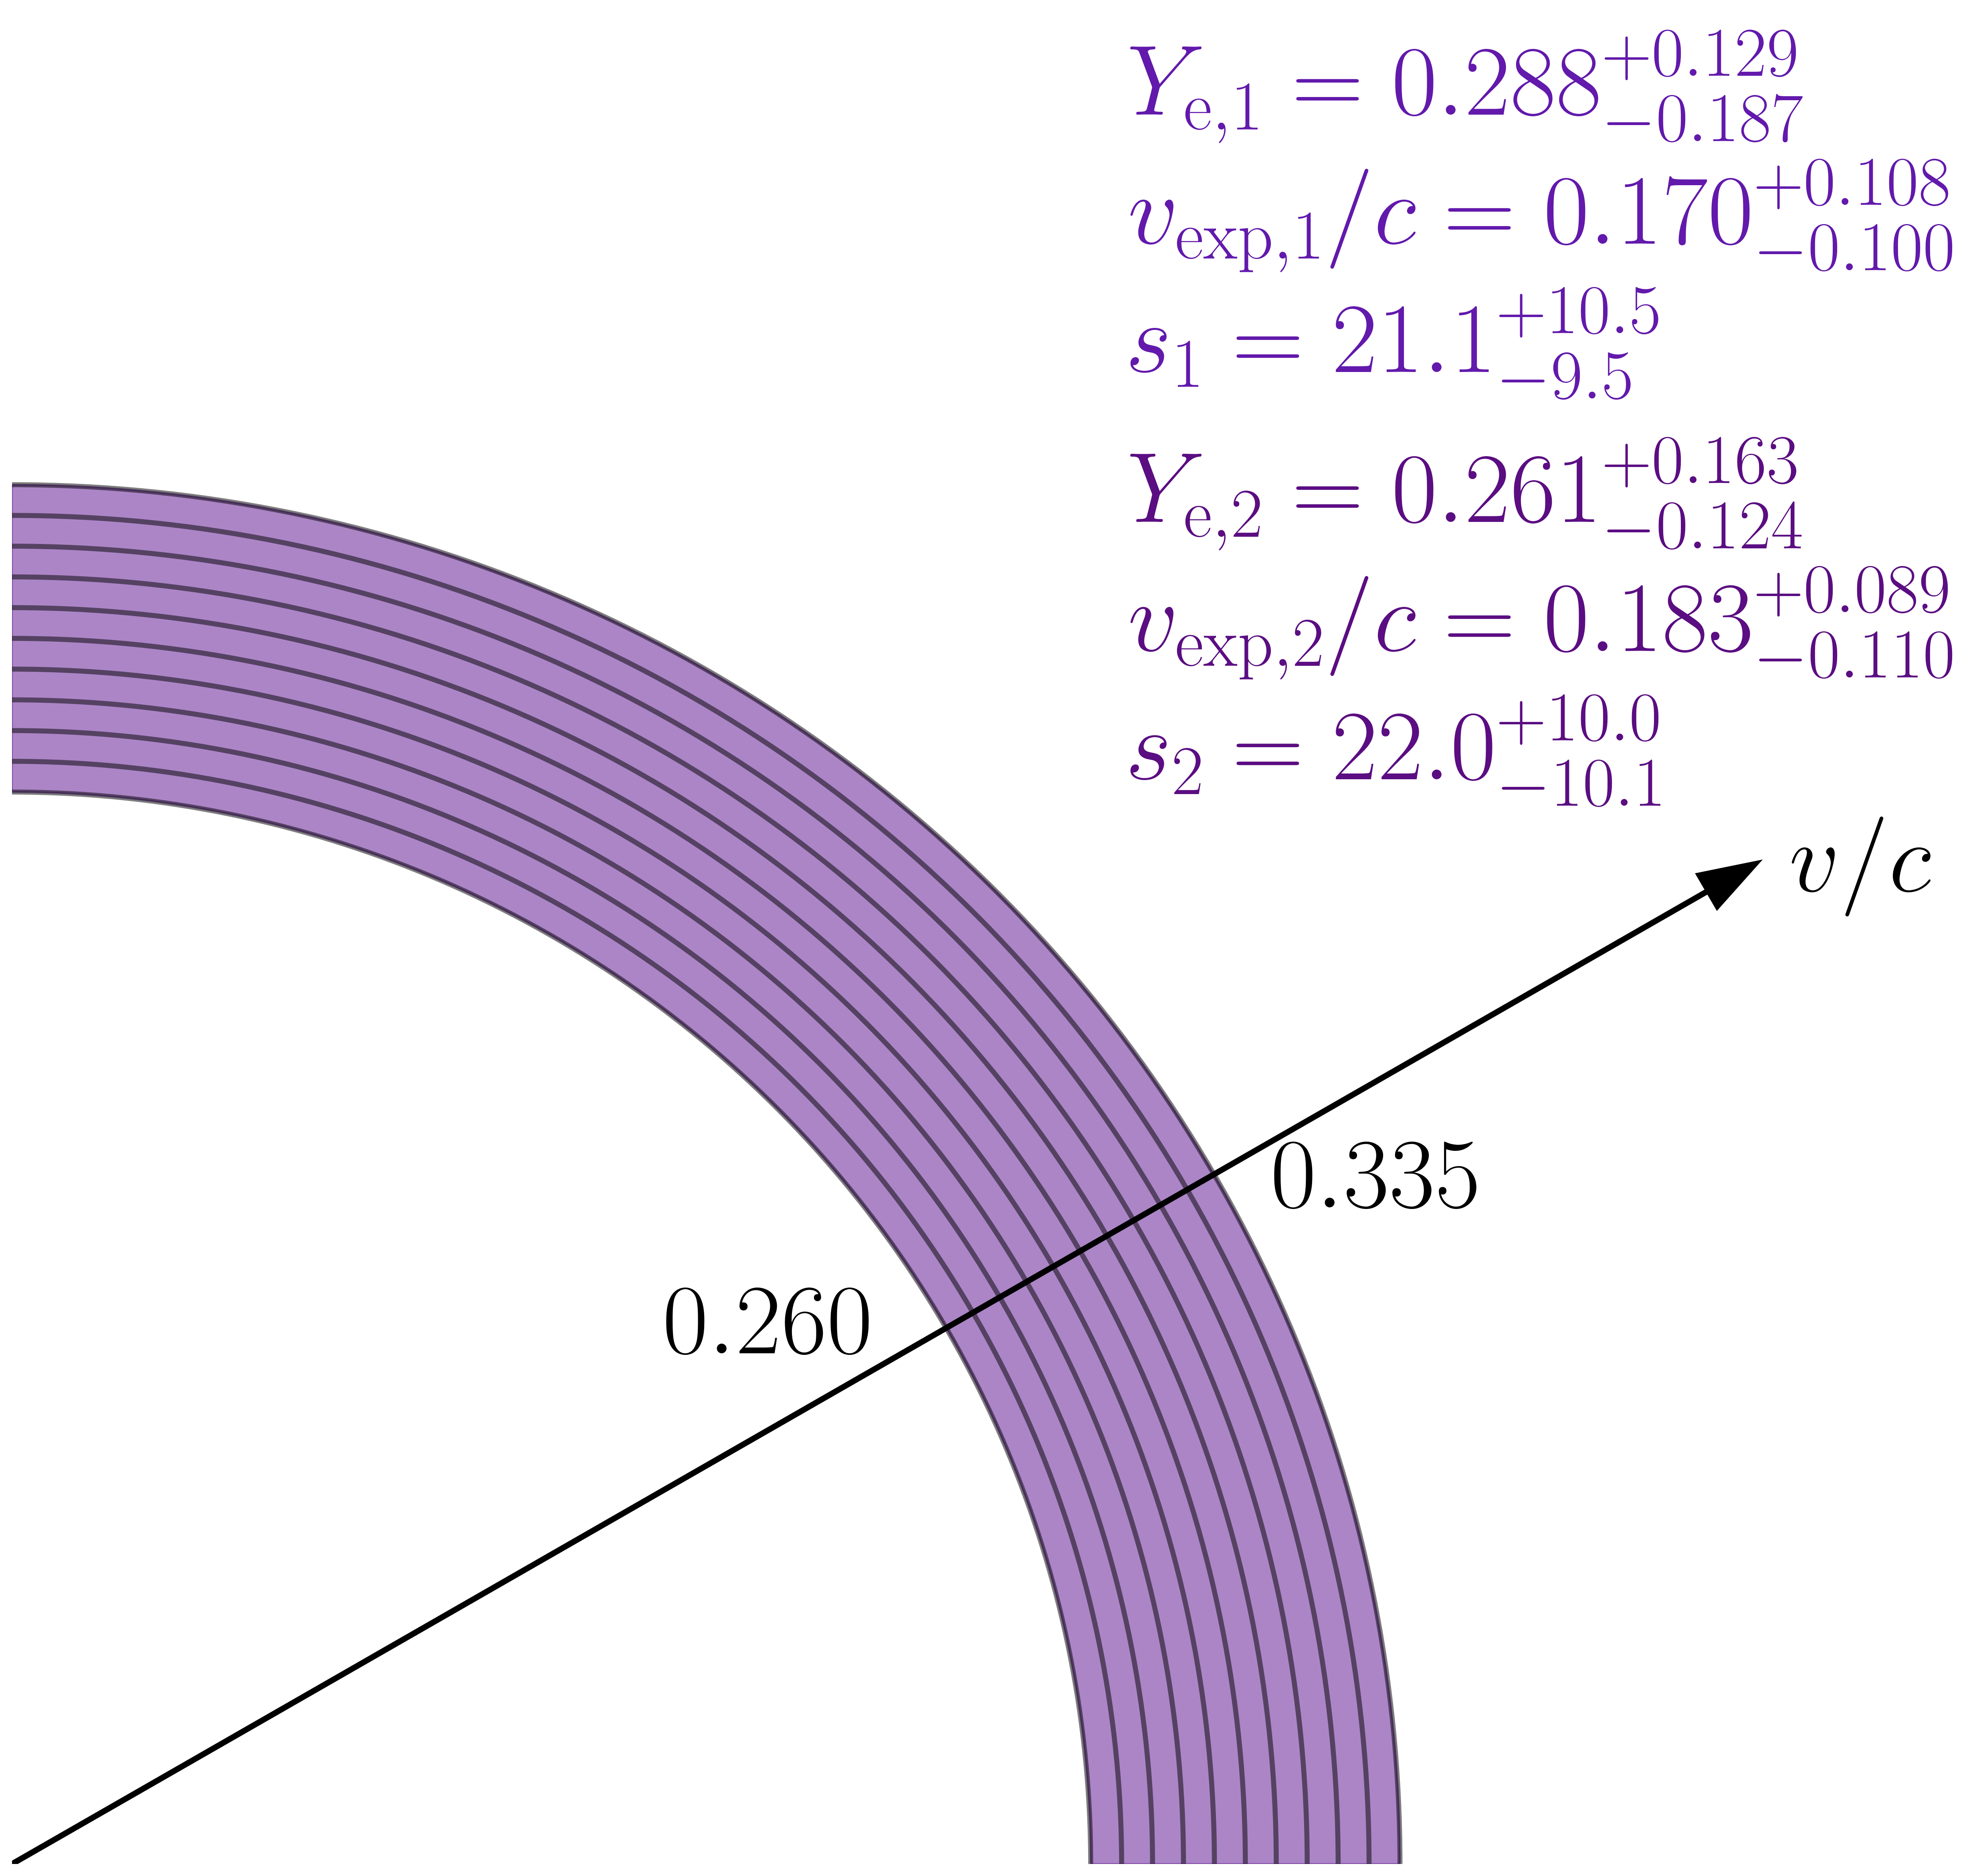
\includegraphics[width=0.4\textwidth]{figs/multicomp_wedges_2.4d.png}
    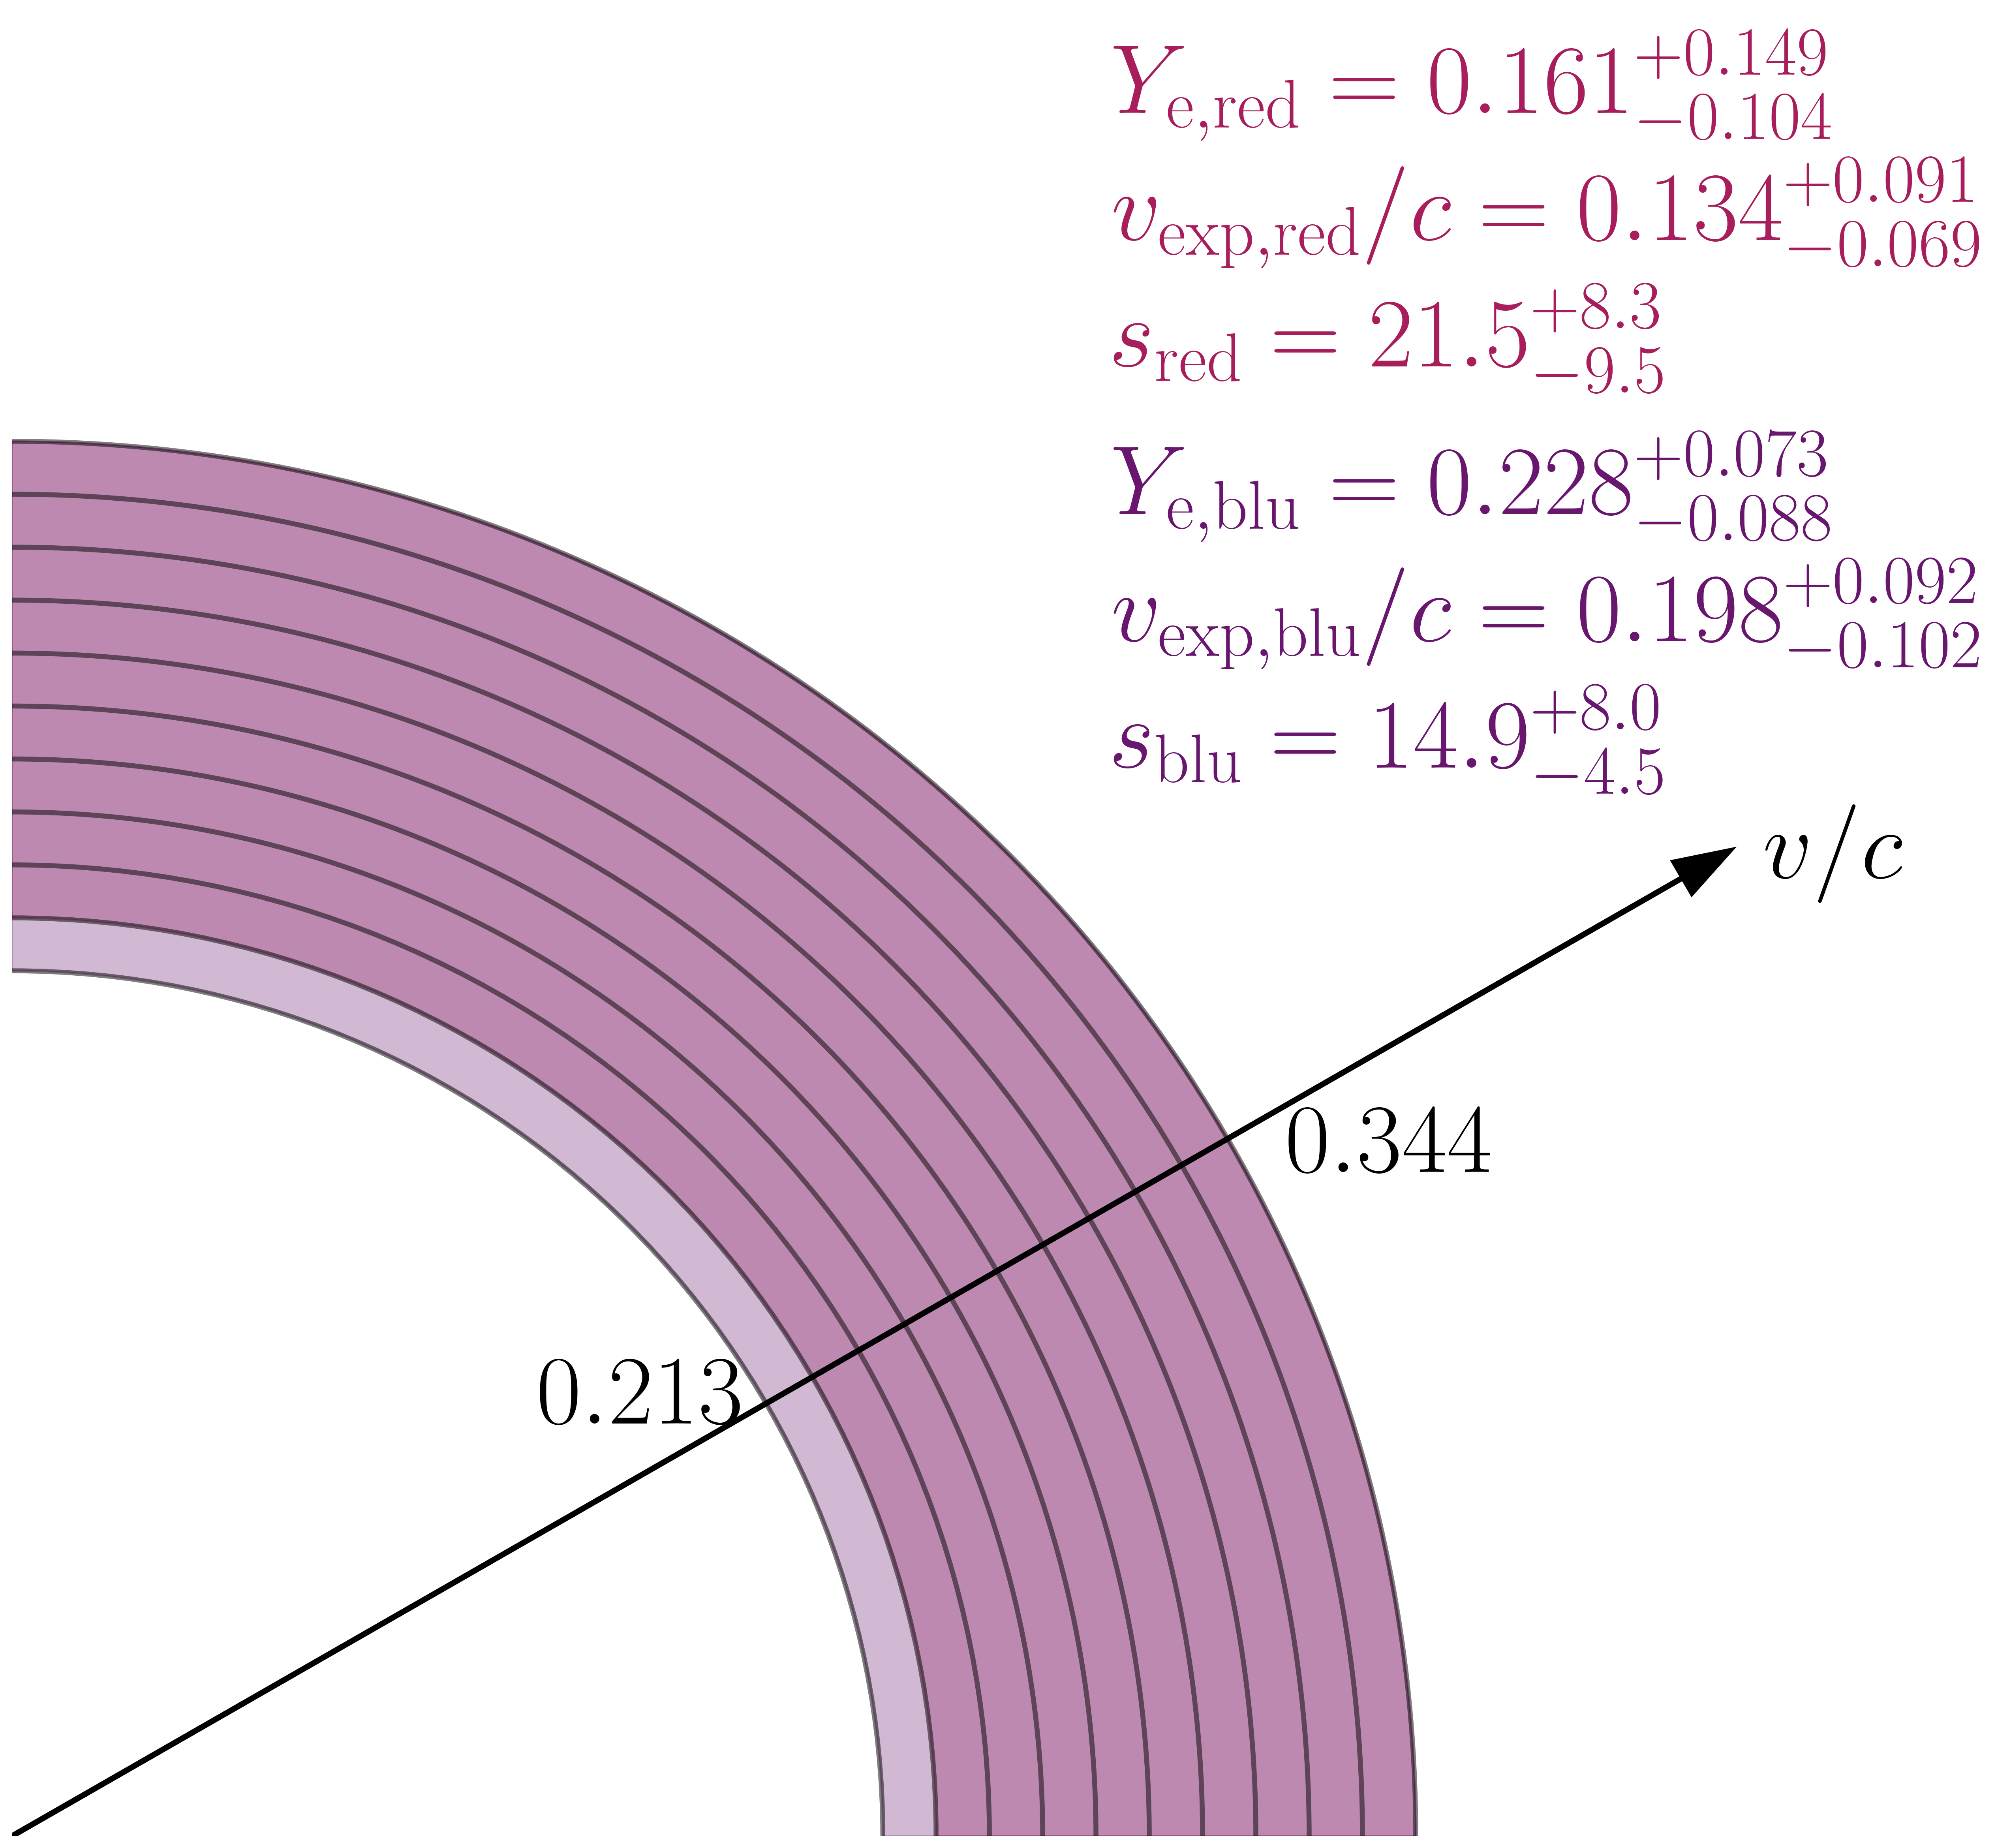
\includegraphics[width=0.4\textwidth]{figs/multicomp_wedges_3.4d.png}
    \figcaption{\textbf{Physical setup and composition-setting parameters for the multi-component models.} Best fits are taken as the median of the posteriors, included in Appendix~\ref{app:corners_multi}). From top to bottom: 1.4, 2.4, and 3.4 days. At 1.4 days, a thin ``red'' component which contains just $\sim4$\% of the total ejecta mass emerges. This component has a negligible impact on the emergent spectrum, and altering its abundance pattern does not significantly impact the fit shown in Figure~\ref{fig:bestfits}, indicating that this model is effectively single-component. At 2.4 days, two components with remarkably similar compositions completely overlap in space, effectively indicating a single-component ejecta. At 3.4 days, two components with different compositions are present.}\label{fig:infer_multicomp_wedges}
\end{figure}


\subsubsection{Multi-component, 1.4 days}\label{sssc:1.4_multi}

We require $m_0 + m_{\mathrm{active}} = 1500 + 1471$ points to obtain a good fit and converged posterior in our 1.4 day, multi-component \SPARK~run. Due to the increased dimensionality of the multi-component fits, more active learning samples are required than for single-component. The resultant fit is of similar quality to the single-component equivalent. However, the depth of the absorption feature (due to Sr) is greater, and the redder wing of the P Cygni feature is more pronounced. However, the fit does not capture the continuum at wavelengths $\gtrsim 10,500$ \AA~or wavelengths in the range $\sim[3500, 5000]$ \AA. The fit does a marginally better job at the shortest wavelengths, $\lesssim 3500$ \AA. 

We infer an outer boundary luminosity of $\log_{10} (L_{\mathrm{outer}}/L_{\odot}) = 7.853^{+0.014}_{-0.023}$, or equivalently, $L_{\mathrm{outer}} = $. This is brighter than is inferred in the single-component equivalent; however, due to the use of 10 radial shells (as opposed to 1) and 30 \TARDIS~iterations (rather than 1), the meaning of $L_{\mathrm{outer}}$ is different and cannot be mapped directly to $T_{\mathrm{inner}}$. 

We find $\log_{10} (\rho_0 / \mathrm{g~cm^{-3}}) = -15.106^{+0.140}_{-0.586}$, or equivalently $\rho_0 = $. The two components in the ejecta are bounded by $v_{\mathrm{inner,1}}/c = 0.322^{+0.007}_{-0.031}$, $v_{\mathrm{outer,1}}/c = 0.325^{+0.009}_{-0.016}$ and $v_{\mathrm{inner,2}}/c = 0.281^{+0.012}_{-0.017}$, $v_{\mathrm{outer,2}}/c = 0.356^{+0.015}_{-0.015}$. This first component is described by electron fraction $Y_{e,1} = 0.133^{+0.033}_{-0.120}$, expansion velocity $v_{\mathrm{exp},1}/c = 0.120^{+0.027}_{-0.026}$, and specific entropy $s_1 / k_{\mathrm{B}} = 24.4^{+3.6}_{-5.3}$, and could thus be described as ``red''. The latter has $Y_{e,2} = 0.338^{+0.021}_{-0.021}$, $v_{\mathrm{exp},2}/c = 0.193^{+0.036}_{-0.037}$, and $s_2 / k_{\mathrm{B}} = 20.0^{+3.9}_{-3.5}$, and is bluer. As in the single-component fits, expansion velocities ($v_{\mathrm{exp},1}$ and $v_{\mathrm{exp},2}$) are poorly constrained. The entropies ($s_1$ and $s_2$) of both components are higher than, and inconsistent with, the single-component equivalent at 1.4 days. However, the $Y_{e,2}$ of the second, bluer component is consistent with that of the single-component equivalent. Indeed, the $(Y_{e,2},~v_{\mathrm{exp},2},~s_2)$ of this bluer component can be replaced by the $(Y_e,~v_{\mathrm{exp}},~s)$ of the purple + warm single-component model at 1.4 days, with minimal impact on the spectrum. 

A physical picture for the components is included in Figure~\ref{fig:infer_multicomp_wedges}. We see that the red is confined to a single shell, while the blue component extends over a greater radius. The mass contained in these two components is $M_1/M_{\odot} = 2.7^{+0.9}_{-3.6} \times 10^{-6}$ and $M_2/M_{\odot} = 6.9^{+2.2}_{-9.3} \times 10^{-5}$, respectively. This second, bluer component thus contains $\sim 25 \times$ as much mass as the redder, and dominates the absorption/emission in the synthetic spectrum. In this sense, we interpret this model as effectively being single-component.



\subsubsection{Multi-component, 2.4 days}\label{sssc:2.4_multi}

As in the 1.4 day, multi-component fit, we require more active learning points than for the single-component equivalent at 2.4 days: we require $m_0 + m_{\mathrm{active}} = 1500 + 1020$ points to obtain a good fit and converged posterior in our 2.4 day, multi-component \SPARK~run. The resultant fit is of similar quality to the single-component equivalent. However, the depth of the absorption feature (due to Sr) is overestimated. The multi-component fit does achieve a better fit to the continuum at wavelengths $\lesssim 7000$ \AA. 

We infer an outer boundary luminosity of $\log_{10} (L_{\mathrm{outer}}/L_{\odot}) = 7.700^{+0.065}_{-0.073}$, or equivalently, $L_{\mathrm{outer}} = $. As expected, the kilonova has dimmed, compared to the 1.4 day, multi-component model. We find $\log_{10} (\rho_0 / \mathrm{g~cm^{-3}}) = -15.440^{+0.813}_{-0.467}$, or equivalently $\rho_0 = $. The two components in the ejecta are bounded by $v_{\mathrm{inner,1}}/c = 0.260^{+0.061}_{-0.039}$, $v_{\mathrm{outer,1}}/c = 0.335^{+0.054}_{-0.065}$ and $v_{\mathrm{inner,2}}/c = 0.268^{+0.049}_{-0.045}$, $v_{\mathrm{outer,2}}/c = 0.335^{+0.045}_{-0.070}$. This first component is described by electron fraction $Y_{e,1} = 0.288^{+0.129}_{-0.187}$, expansion velocity $v_{\mathrm{exp},1}/c = 0.170^{+0.108}_{-0.100}$, and specific entropy $s_1 / k_{\mathrm{B}} = 21.1^{+10.5}_{-9.5}$, while the latter has $Y_{e,2} = 0.261^{+0.163}_{-0.124}$, $v_{\mathrm{exp},2}/c = 0.183^{+0.089}_{-0.110}$, and $s_2 / k_{\mathrm{B}} = 22.0^{+10.0}_{-10.1}$. Again, expansion velocities are poorly constrained, and entropies are higher than, and inconsistent with, the single-component equivalent at 2.4 days. However, both entropies are consistent with the entropies inferred in the 1.4 day, multi-component model. Finally, $Y_{e,1}$ and $Y_{e,2}$ are both lower than, but still consistent with, that of the dominant blue component in the 1.4 day, multi-component model and the 1.4 day, single-component model. Once again, we can swap out the bluer $(Y_{e,1},~v_{\mathrm{exp},1},~s_1)$ component of the model for the $(Y_e,~v_{\mathrm{exp}},~s)$ of the purple + warm single-component model at 1.4 days, with minimal impact on the spectrum. 

A physical picture for the components is included in Figure~\ref{fig:infer_multicomp_wedges}. The two components almost completely overlap in physical space. Indeed, the mass contained in these two components is $M_1/M_{\odot} = 3.4^{+6.4}_{-3.7} \times 10^{-5}$ and $M_2/M_{\odot} = 3.0^{+5.6}_{-3.3} \times 10^{-5}$, respectively; the ejecta is effectively equally partitioned into these two components. Furthermore, the similarity between $(Y_{e,1},~v_{\mathrm{exp},1},~s_1)$ and $(Y_{e,2},~v_{\mathrm{exp},2},~s_2)$ yields similar compositions for both components. For these reasons, we also interpret this model as effectively being single-component.



\subsubsection{Multi-component, 3.4 days}\label{sssc:3.4_multi}

x



%%% subsection: ABUNDANCES
\subsection{Abundances of favored models}\label{ssc:results-abundances}


%% abundance patterns; Fig. 3
\begin{figure*}[!ht]
    \centering
    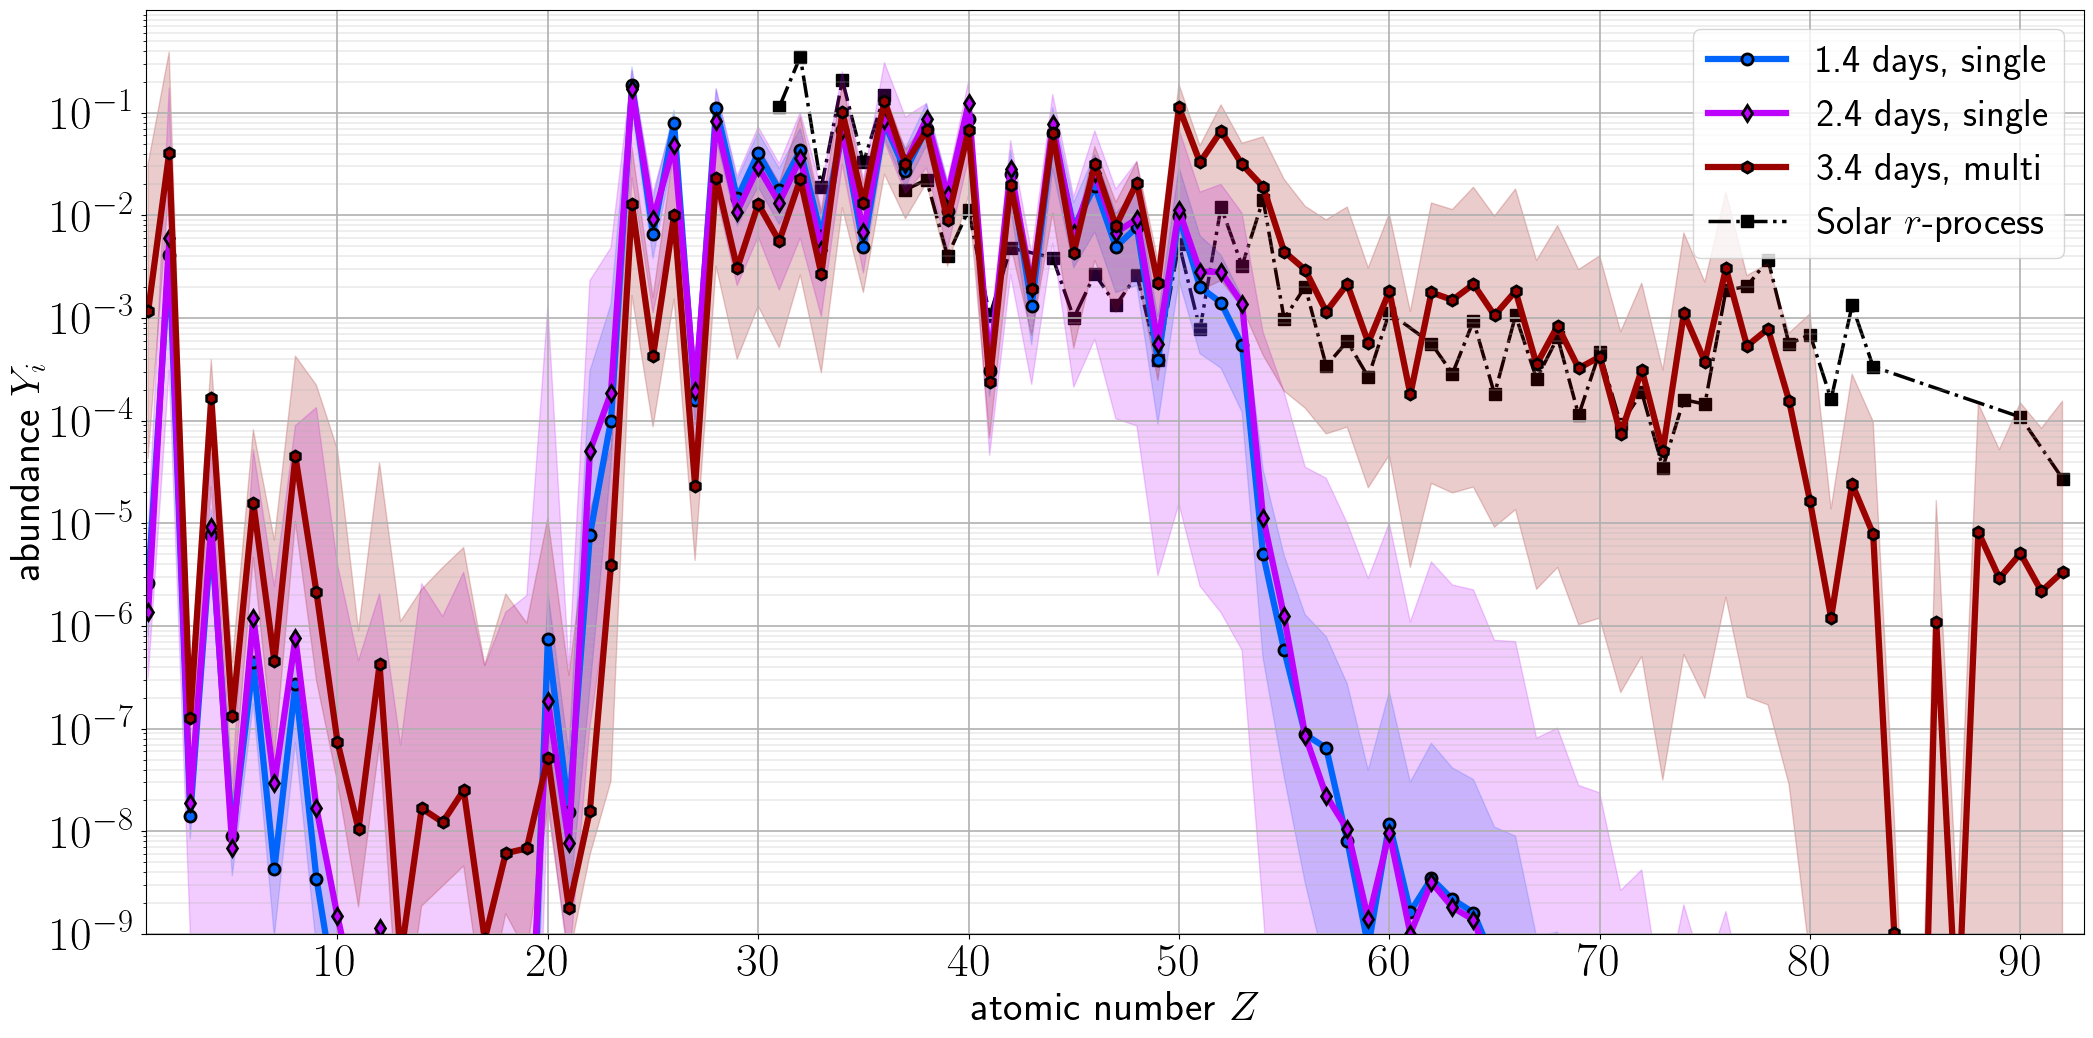
\includegraphics[width=0.98\textwidth]{figs/compare_abunds_220808_014638-221022_084052-230622_230103_posterior_100samples_dynesty.png}
    \figcaption{\textbf{Best-fit abundance patterns at 1.4, 2.4, and 3.4 days.} The abundances at 1.4 and 2.4 days are taken from the preferred single-component fits, while the abundance at 3.4 days is taken from the multi-component fit. The overall abundance of the multi-component ejecta at 3.4 days is the mass-weighted sum over all 10 shells in the stratified ejecta. A new, redder kilonova component emerges at 3.4 days post-merger. Uncertainty bands are obtained by taking additional samples from the the posterior, effectively propagating the uncertainty on $Y_e$, $v_{\mathrm{exp}}$, and $s$ into the abundances. We also show the Solar $r$-process pattern, computed using data from \cite{lodders09} subtracted by the $s$-process residuals of \cite{bisterzo14}. The best-fit abundances are evidently non-Solar at the first two epochs, but are closer to Solar at the third. }\label{fig:abunds_time_evolution}
\end{figure*}


%%% subsection: LoO AND SDEC
\subsection{Elements present in favored models}\label{ssc:results-lines}


%%% leave-one-out spectra; Fig. 4
\begin{figure}[!ht]
    \centering
    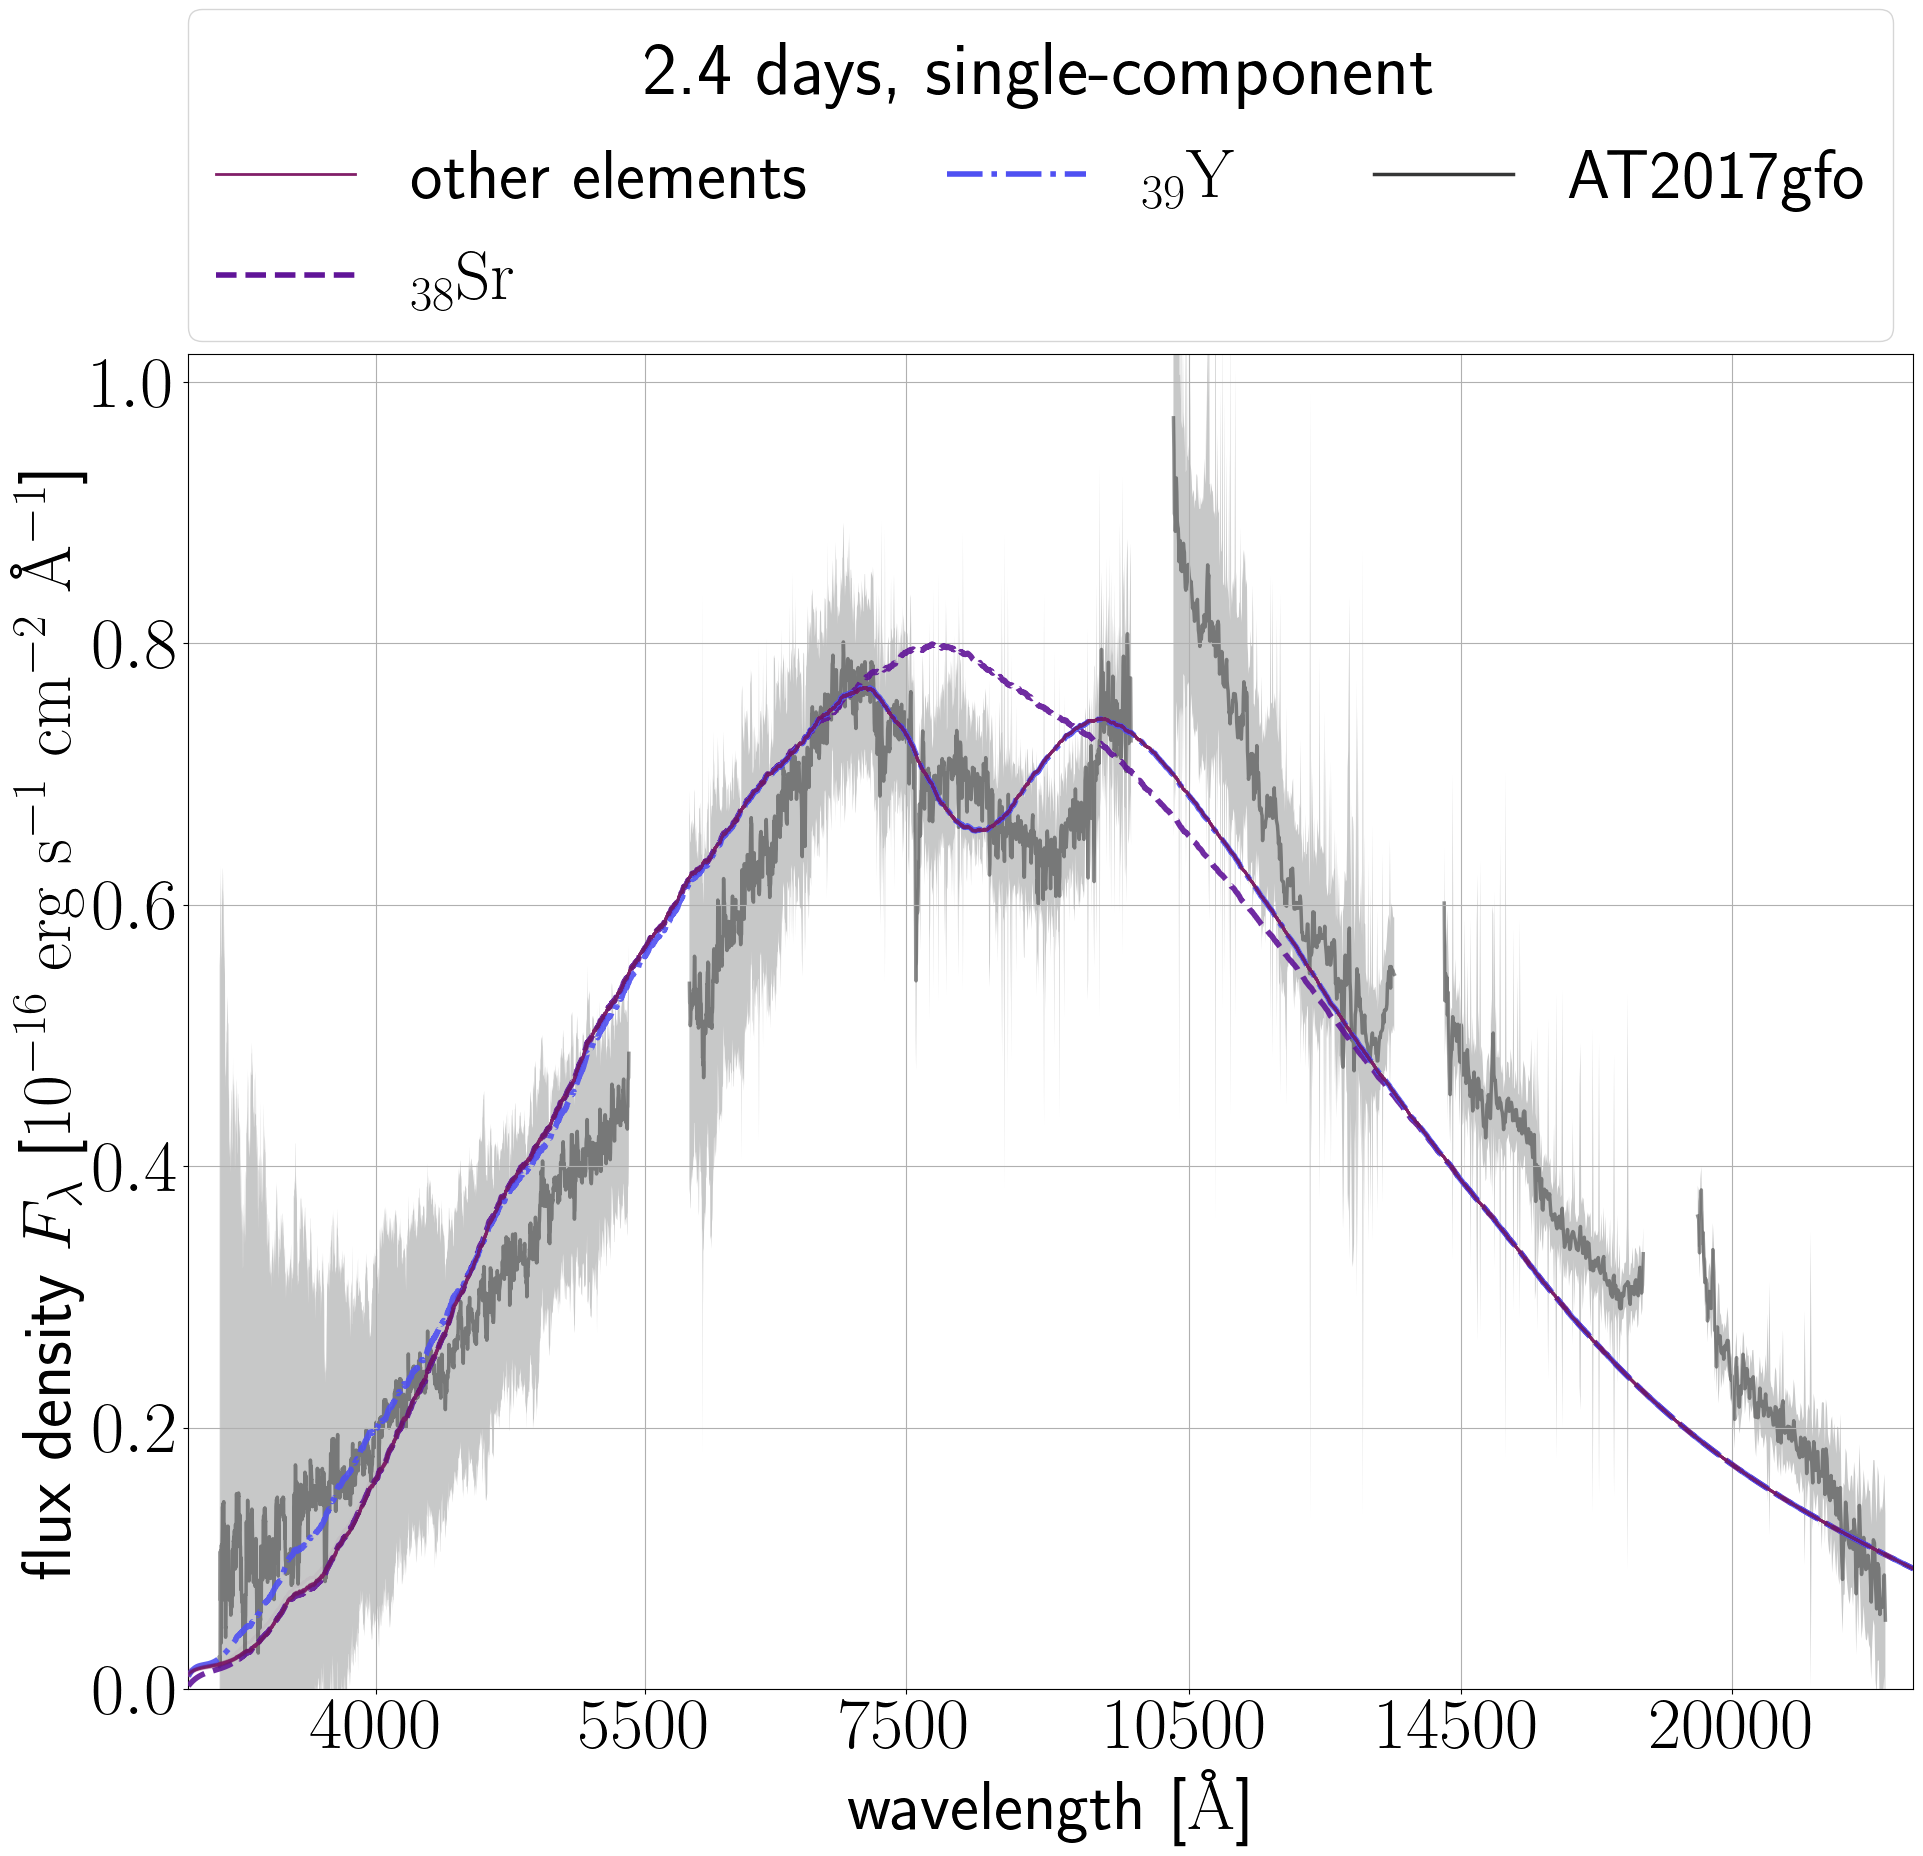
\includegraphics[width=0.47\textwidth]{figs/230409_234104_leaveoneout_all_TARDIS_evals_label-interest-38-39.png}
    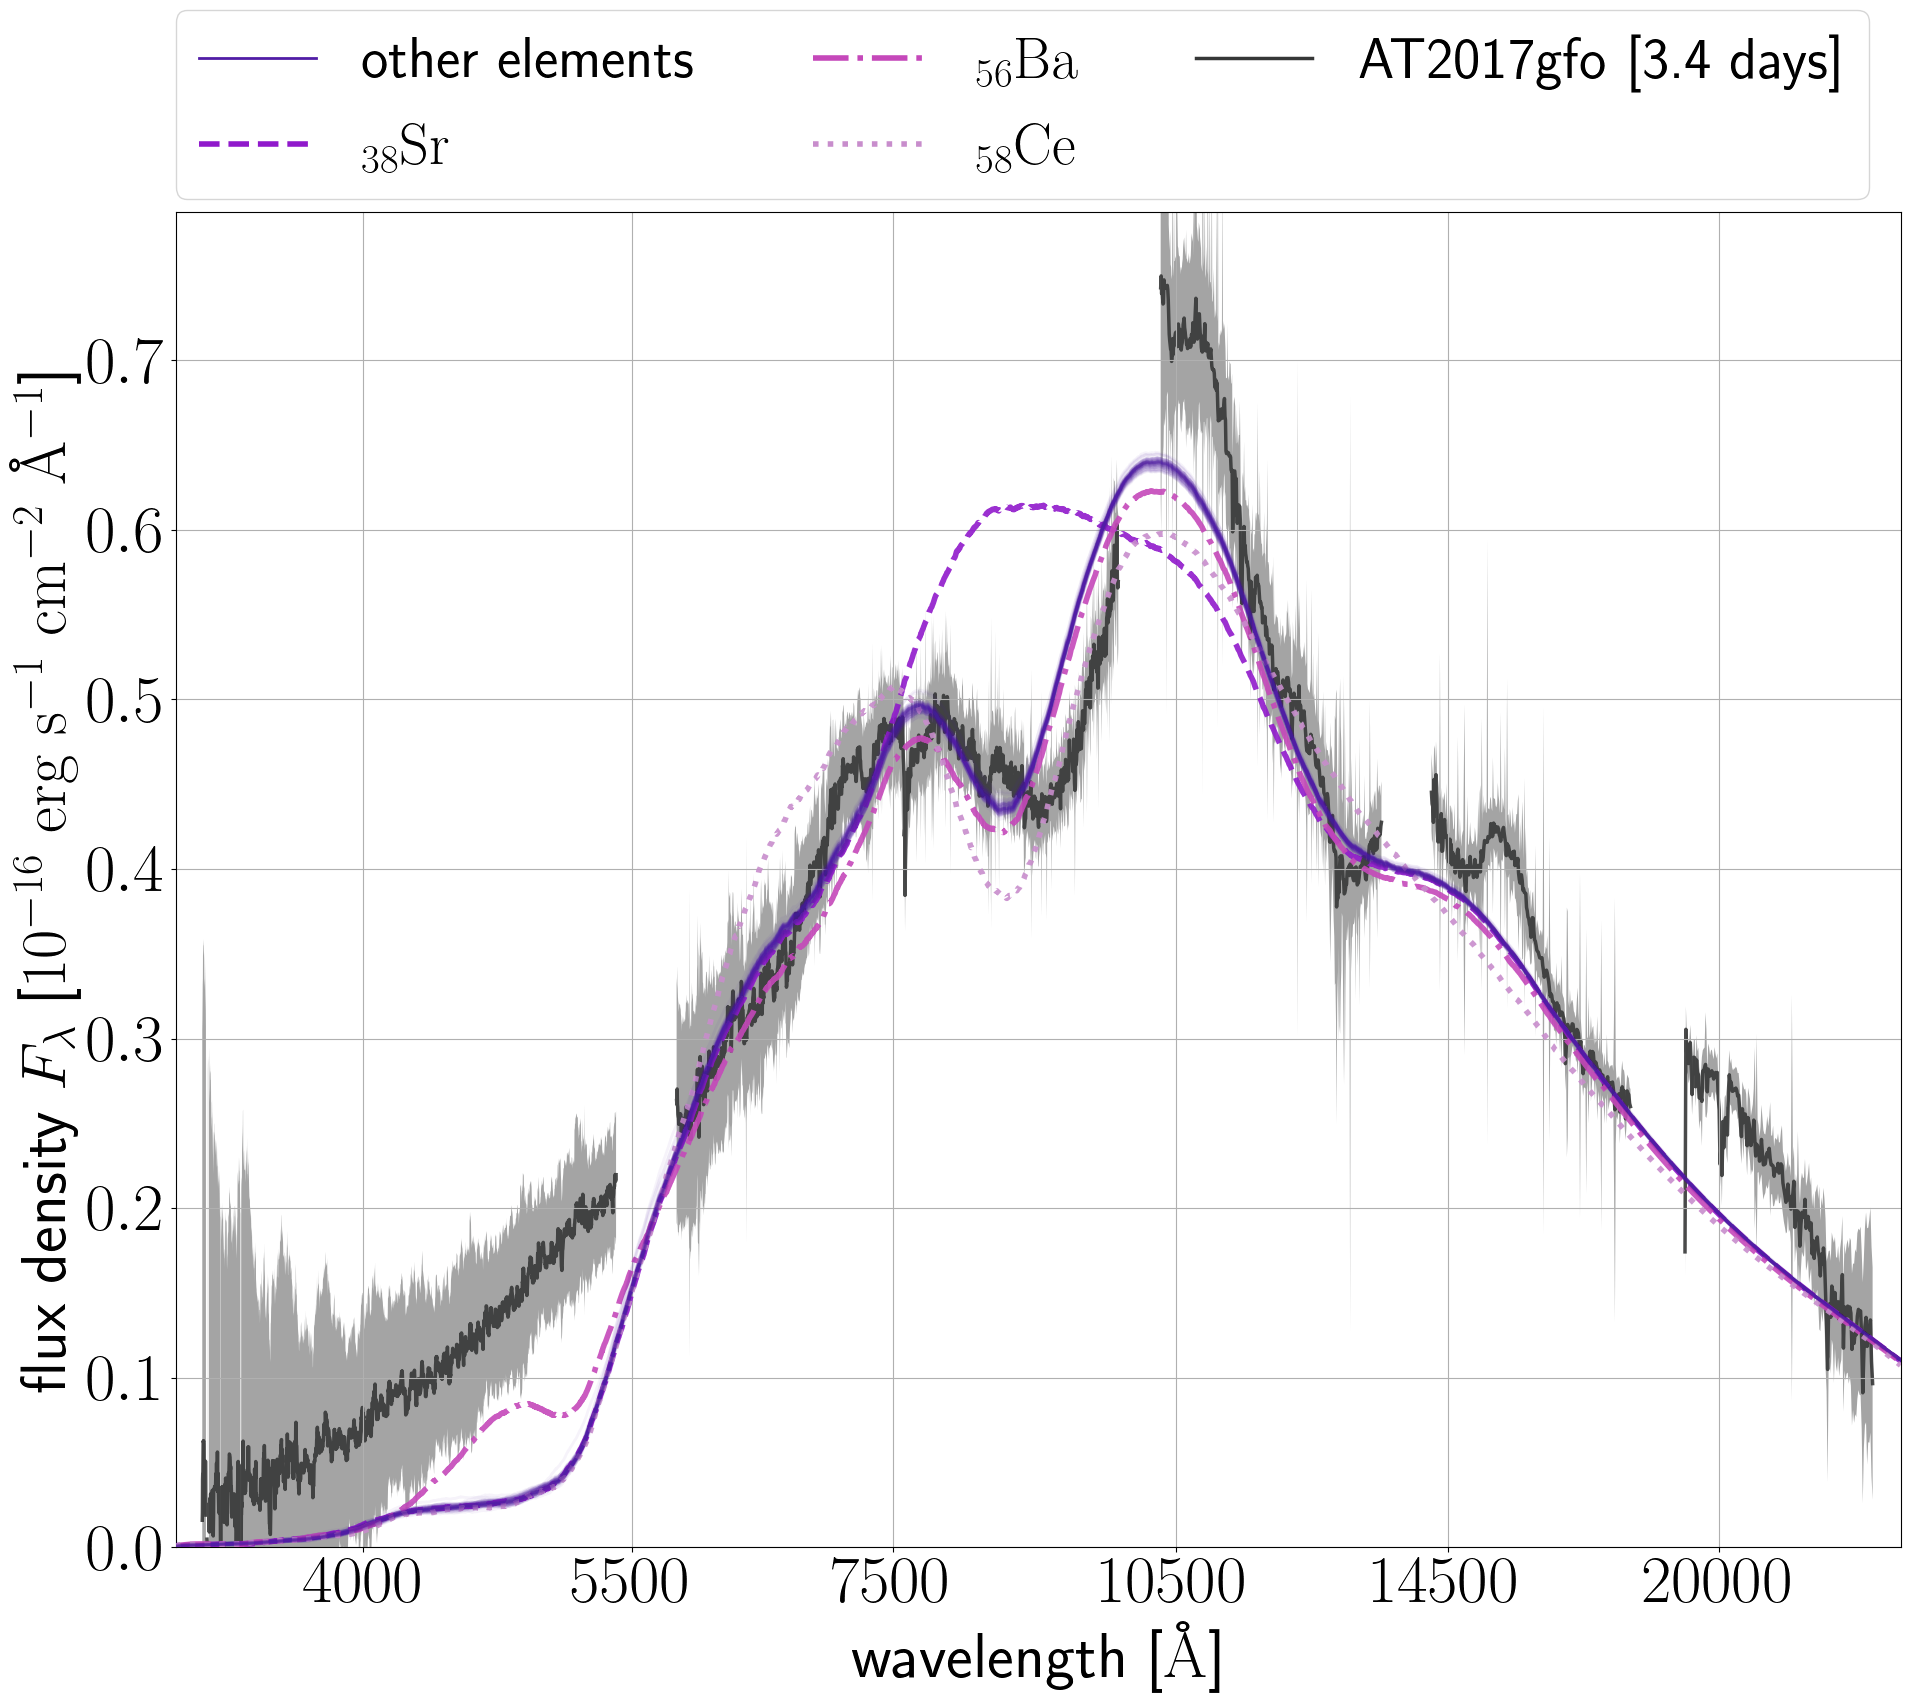
\includegraphics[width=0.47\textwidth]{figs/230626_170245_leaveoneout_all_TARDIS_evals_label-interest-38-56-58.png}
    \figcaption{\textbf{Leave-one-out spectra for the favored, new models: single-component for 2.4 days, and multi-component for 3.4 days.} The preferred model for 1.4 days, not shown here, is the single-component purple+warm model of V23. All models (including at 1.4 days, V23) show clear absorption from strontium (${}_{38}$Sr) at $\sim8000$\AA. At 3.4 days, when the abundances included heavier elements, we see an over-absorption from barium (${}_{56}$Ba; an open $s$-shell element in the same group as Sr in the periodic table) at $\sim4500$\AA. We also see absorption (at $\sim7000$\AA) and emission (at $\sim8000$\AA) from the lanthanide cerium (${}_{58}$Ce) at this epoch. Spectral DEComposition (SDEC) plots, included in Appendix~\ref{app:SDEC}, provide a complementary view of the dominant species to these leave-one-out plots.}\label{fig:leave_out_pref}
\end{figure}


%%% === SECTION 4 === %%%
%% DISCUSSION %%

\section{Discussion}\label{sec:disco}


%%% subsection: SINGLE- VERSUS MULTI-COMPONENT MODELS
\subsection{Single- versus multi-component}


%%% subsection: TIME EVOLUTION OF THE ABUNDANCES
\subsection{Time evolution of the abundances}






%%% === SECTION 5 === %%%
%% CONCLUSIONS %%

\section{Conclusions}\label{sec:conco}



%%% === ACKNOWLEDGEMENTS === %%%
\acknowledgments


NV works in Tiohti{\'a}:ke / Mooniyang, also known as Montr{\'e}al, which lies on the unceded land of the Haudenosaunee and Anishinaabeg nations. This work made use of high-performance computing resources in Tiohti{\'a}:ke / Mooniyang and in Burnaby, British Columbia, the unceded land of the Coast Salish peoples, including the Tsleil-Waututh, Kwikwetlem, Squamish, and Musqueam nations. We acknowledge the ongoing struggles of Indigenous peoples on this land, and elsewhere on Turtle Island, and hope for a future marked by true reconciliation. 

We thank the attendees of an April 2023 workshop at University of California---Santa Cruz, and especially Erika Holmbeck, Phil Macias, and Ashley Villar, for fruitful discussions on kilonovae and the $r$-process. We are also grateful to Shinya Wanajo for kindly sharing their reaction network calculations. Finally, we thank Jessica Birky and David Fleming for useful discussions on approximate Bayesian inference and the use of \href{https://dflemin3.github.io/approxposterior/index.html}{\approxposterior}.

This work made extensive use of the \href{https://docs.alliancecan.ca/wiki/Narval/en}{\texttt{Narval}} and \href{https://docs.alliancecan.ca/wiki/Cedar}{\texttt{Cedar}} clusters of the \href{https://alliancecan.ca/en}{Digital Research Alliance of Canada} at the {\'E}cole de technologie sup{\'e}rieure and Simon Fraser University (with regional partner \href{https://www.westgrid.ca/}{WestGrid}), respectively. We thank the support staff of Calcul Qu{\'e}bec in particular for their assistance at various steps in this project. 

This work has made use of the \href{http://vald.astro.uu.se/~vald/php/vald.php}{Vienna Atomic Line Database (VALD)}, operated at Uppsala University, the Institute of Astronomy RAS in Moscow, and the University of Vienna. We thank Nikolai Piskunov and Eric Stempels for help in obtaining the VALD data.

This research made use of \href{https://tardis-sn.github.io/tardis/index.html}{\TARDIS}, a community-developed software package for spectral synthesis in supernovae (\citealt{kerzendorf14}). The development of \TARDIS~received support from the Google Summer of Code initiative and from the European Space Agency (ESA)'s Summer of Code in Space program. \TARDIS~makes extensive use of \href{https://docs.astropy.org/en/stable/}{\texttt{astropy}}. We thank Andrew Fullard, Wolfgang Kerzendorf, and the entire \TARDIS~development team for their assistance and their commitment to the development and maintenance of the code. 

N.V. acknowledges funding from the National Sciences and Engineering Research Council of Canada (NSERC) Canada Graduate Scholarship - Doctoral (CGS-D), the Murata Family Fellowship, and the the Bob Wares Science Innovation Prospectors Fund. J.J.R.\ and D.H.\ acknowledge support from the Canada Research Chairs (CRC) program, the NSERC Discovery Grant program, the FRQNT Nouveaux Chercheurs Grant program, and the Canadian Institute for Advanced Research (CIFAR). J.J.R.\ acknowledges funding from the Canada Foundation for Innovation (CFI), and the Qu\'{e}bec Ministère de l’\'{E}conomie et de l’Innovation. \redbf{N.M.F. acknowledgements.}
\newline

%%% === SOFTWARE === %%%
\software{
\href{https://dflemin3.github.io/approxposterior/index.html}{\approxposterior}: \cite{fleming18};
\href{https://docs.astropy.org/en/stable/}{\texttt{astropy}}: \cite{astropy18};
\href{https://cmasher.readthedocs.io/}{\texttt{cmasher}}: \cite{velden20};
\href{https://corner.readthedocs.io/en/latest/index.html}{\texttt{corner}}: \cite{foreman-mackey16};
\href{https://dynesty.readthedocs.io/en/latest/index.html}{\texttt{dynesty}}: 
\cite{speagle20};
% \href{https://emcee.readthedocs.io/en/stable/}{\texttt{emcee}}: \cite{foreman-mackey13}; 
\href{https://george.readthedocs.io/en/latest/}{\texttt{george}}: \cite{ambikasaran15};
\href{https://tardis-sn.github.io/tardis/index.html}{\TARDIS}: \cite{kerzendorf14};
\href{https://johannesbuchner.github.io/UltraNest/}{\texttt{UltraNest}}: \cite{buchner21}
} 

\clearpage



%%% === BIBLIOGRAPHY === %%%
\bibliographystyle{apj}
\begin{thebibliography}{}


%\bibitem[Abbott \& Lucy(1985)]{abbott85} Abbott, D.~C. \& Lucy, L.~B.\ 1985, \apj, 288, 679
%%%%% TARDIS LUCY FORMALISM


% \bibitem[Abbott et al.(2017a)]{abbottLIGO17a} Abbott, B.~P., Abbott, R., Abbott, T.~D., et al.\ 2017a, \aj, 848, L12
% %%%%% G170817: MULTI-MESSENGER


% \bibitem[Abbott et al.(2017b)]{abbottLIGO17b} Abbott, B.~P., Abbott, R., Abbott, T.~D., et al.\ 2017b, \apjl, 848, L13
% %%%%% GW170817: GWs AND GRBs


% \bibitem[Abbott et al.(2017)]{abbott17c} Abbott, B.~P., Abbott, R., Abbott, T.~D., et al.\ 2017, \prl, 119, 161101
% %%%%% GW170817: GWs 

%\bibitem[Abbott et al.(2018)]{abbottLIGO18} Abbott, B.~P., Abbott, R., Abbott, T.~D., et al.\ 2018, Living Reviews in Relativity, 21, 3


%\bibitem[Abbott et al.(2018)]{abbott18} Abbott, T.~M.~C., Abdalla, F.~B., Allam, S., et al.\ 2018, \apjs, 239, 18


% \bibitem[Ai et al.(2022)]{ai22} Ai, S., Zhang, B., \& Zhu, Z.\ 2022, \mnras, 516, 2614


% \bibitem[Almualla et al.(2021)]{almualla21} Almualla, M., Ning, Y., Bulla, M., et al.\ 2021, arXiv:2112.1547
% %%%%% INFERENCE WITH POSSIS



\bibitem[Ambikasaran et al.(2015)]{ambikasaran15} Ambikasaran, S., Foreman-Mackey, D., Greengard, L., et al.\ 2015, IEEE Transactions on Pattern Analysis and Machine Intelligence, 38, 252


% \bibitem[Anand et al.(2021)]{anand21} Anand, S., Coughlin, M.~W., Kasliwal, M.~M., et al.\ 2021, Nature Astronomy, 5, 46
% %%%%% POSSIS DATASET USED IN LUKOSIUTE+22


% \bibitem[Andreoni et al.(2017)]{andreoni17} Andreoni, I., Ackley, K., Cooke, J., et al.\ 2017, \pasa, 34, e069
% %%%%% GW170817 OBSERVATIONS


% \bibitem[Arcavi et al.(2017)]{arcavi17} Arcavi, I., Hosseinzadeh, G., Howell, D.~A., et al.\ 2017, \nat, 551, 64
% %%%%% GW170817 OBSERVATIONS


%\bibitem[Arnett(1982)]{arnett82} Arnett, W.~D.\ 1982, \apj, 253, 785


\bibitem[Astropy Collaboration et al.(2018)]{astropy18} Astropy Collaboration, Price-Whelan, A.~M., Sip{\H{o}}cz, B.~M., et al.\ 2018, \aj, 156, 123


% \bibitem[Badnell(2016)]{badnell16} Badnell, N.~R.\ 2016, AUTOSTRUCTURE: General program for calculation of atomic and ionic properties, ascl:1612.014


% \bibitem[Baiotti \& Rezzolla(2017)]{baiotti17} Baiotti, L. \& Rezzolla, L.\ 2017, Reports on Progress in Physics, 80, 096901.


%\bibitem[Banerjee et al.(2020)]{banerjee20} Banerjee, P., Wu, M.-R., \& Yuan, Z.\ 2020, \apjl, 902, L34
%%%%% ASTROPHYSICAL SITE OF THE R-PROCESS


%\bibitem[Bar-Shalom et al.(2001)]{barshalom01} Bar-Shalom, A., Klapisch, M., \& Oreg, J.\ 2001, \jqsrt, 71, 169


%\bibitem[Barnes \& Kasen(2013)]{barnes13} Barnes, J., Kasen, D.\ 2013, \aj, 775, 18


% \bibitem[Barnes et al.(2016)]{barnes16} Barnes, J., Kasen, D., Wu, M., Mart\'{i}nez-Pinedo, G.\ 2016, \apj, 829, 110


% \bibitem[Barnes et al.(2021)]{barnes21} Barnes, J., Zhu, Y.~L., Lund, K.~A., et al.\ 2021, \apj, 918, 44


%\bibitem[Barstow \& Heng(2020)]{barstow20} Barstow, J.~K., \& Heng, K.\ 2020, arXiv e-prints, arXiv:2003.14311


% \bibitem[Bartos \& Marka(2019)]{bartos19} Bartos, I. \& Marka, S.\ 2019, \nat, 569, 85
% %%%%% ASTROPHYSICAL SITE OF THE R-PROCESS


% \bibitem[Bauswein et al.(2013)]{bauswein13} Bauswein, A., Goriely, S., \& Janka, H.-T.\ 2013, \apj, 773, 78



% \bibitem[Beniamini et al.(2016)]{beniamini16} Beniamini, P., Hotokezaka, K., \& Piran, T.\ 2016, \apj, 832, 149
% %%%%% ASTROPHYSICAL SITE OF THE R-PROCESS


%\bibitem[Bethe \& Brown(1998)]{bethe98} Bethe, H.~A., \& Brown, G.~E.\ 1998, \apj, 506, 780

\bibitem[Bisterzo et al.(2014)]{bisterzo14} Bisterzo, S., Travaglio, C., Gallino, R., et al.\ 2014, \apj, 787, 10


% \bibitem[Brauer et al.(2020)]{brauer20} Brauer, K., Ji, A.~P., Drout, M.~R., et al.\ 2020, arXiv:2010.15837
% %%%%% ASTROPHYSICAL SITE OF THE R-PROCESS


\bibitem[Buchner(2021)]{buchner21} Buchner, J.\ 2021, The Journal of Open Source Software, 6, 3001
%%%%% ULTRANEST


% \bibitem[Bulla(2019)]{bulla19} Bulla, M.\ 2019, \mnras, 489, 5037


% \bibitem[Burbidge et al.(1957)]{burbidge57} Burbidge, E.~M., Burbidge, G.~R., Fowler, W.~A., et al.\ 1957, Reviews of Modern Physics, 29, 547


% \bibitem[Cameron(1957)]{cameron57} Cameron, A.~G.~W.\ 1957, \pasp, 69, 201


%\bibitem[Castor(1974)]{castor74} Castor, J.~L.\ 1974, \mnras, 169, 279
%%%%% EXPANSION OPACITY FORMALISM


% \bibitem[Chornock et al.(2017)]{chornock17} Chornock, R., Berger, E., Kasen, D., et al.\ 2017, \apjl, 848, L19


%\bibitem[Christie et al.(2019)]{christie19} Christie, I.~M., Lalakos, A., Tchekhovskoy, A., et al.\ 2019, \mnras, 490, 4811


% \bibitem[Ciolfi(2020)]{ciolfi20a} Ciolfi, R.\ 2020, General Relativity and Gravitation, 52, 59
% %%%%% IMPORTANCE OF B-FIELDS


% \bibitem[Ciolfi \& Kalinani(2020)]{ciolfi20b} Ciolfi, R. \& Kalinani, J.~V.\ 2020, \apjl, 900, L35
% %%%%% B-DRIVEN WIND FOR GW170817


% \bibitem[C{\^o}t{\'e} et al.(2018)]{cote18} C{\^o}t{\'e}, B., Fryer, C.~L., Belczynski, K., et al.\ 2018, \apj, 855, 99
% %%%%% ASTROPHYSICAL SITE OF THE R-PROCESS


% \bibitem[C{\^o}t{\'e} et al.(2019)]{cote19} C{\^o}t{\'e}, B., Eichler, M., Arcones, A., et al.\ 2019, \apj, 875, 106
% %%%%% ASTROPHYSICAL SITE OF THE R-PROCESS


% \bibitem[C{\^o}t{\'e} et al.(2021)]{cote21} C{\^o}t{\'e}, B., Eichler, M., Yag{\"u}e L{\'o}pez, A., et al.\ 2021, Science, 371, 945
% %%%%% ASTROPHYSICAL SITE OF THE R-PROCESS


% \bibitem[Coulter et al.(2017)]{coulter17} Coulter, D.~A., Foley, R.~J., Kilpatrick, C.~D., et al.\ 2017, Science, 358, 1556
% %%%%% GW170817 OBSERVATIONS


%\bibitem[Cowan \& Griffin(1976)]{cowan76} Cowan, R.~D. \& Griffin, D.~C.\ 1976, Journal of the Optical Society of America (1917-1983), 66, 1010
%%%%% AUTOSTRUCTURE CALCULATIONS


\bibitem[Cowan et al.(2021)]{cowan21} Cowan, J.~J., Sneden, C., Lawler, J.~E., et al.\ 2021, Reviews of Modern Physics, 93, 015002
% %%%%% ASTROPHYSICAL SITE OF THE R-PROCESS


% \bibitem[Cunha et al.(2017)]{cunha17} Cunha, K., Smith, V.~V., Hasselquist, S., et al.\ 2017, \apj, 844, 145
% %%%% APOGEE


\bibitem[Czekala et al.(2015)]{czekala15} Czekala, I., Andrews, S.~M., Mandel, K.~S., et al.\ 2015, \apj, 812, 128


% \bibitem[Darbha \& Kasen(2020)]{darbha20} Darbha, S. \& Kasen, D.\ 2020, \apj, 897, 150


% \bibitem[D{\'\i}az et al.(2017)]{diaz17} D{\'\i}az, M.~C., Macri, L.~M., Garcia Lambas, D., et al.\ 2017, \apjl, 848, L29
% %%%%% GW170817 OBSERVATIONS


% \bibitem[Dietrich et al.(2020)]{dietrich20} Dietrich, T., Coughlin, M.~W., Pang, P.~T.~H., et al.\ 2020, Science, 370, 1450
% %%%%% POSSIS DATASET USED IN LUKOSIUTE+22


\bibitem[Domoto et al.(2021)]{domoto21} Domoto, N., Tanaka, M., Wanajo, S., et al.\ 2021, \apj, 913, 26


\bibitem[Domoto et al.(2022)]{domoto22} Domoto, N., Tanaka, M., Kato, D., et al.\ 2022, arXiv:2206.04232


% \bibitem[Drout et al.(2017)]{drout17} Drout, M.~R., Piro, A.~L., Shappee, B.~J., et al.\ 2017, Science, 358, 6370, 1570-1574
% %%%%% GW170817 OBSERVATIONS


%\bibitem[Eastman \& Pinto(1993)]{eastman93} Eastman, R.~G. \& Pinto, P.~A.\ 1993, \apj, 412, 731
%%%%% EXPANSION OPACITY FORMALISM


% \bibitem[Eichler et al.(1989)]{eichler89} Eichler, D., Livio, M., Piran, T., et al.\ 1989, \nat, 340, 126
% %%%%% HISTORICAL RE. NSMs


% \bibitem[Eichler et al.(2015)]{eichler15} Eichler, M., Arcones, A., Kelic, A., et al.\ 2015, \apj, 808, 30


% \bibitem[Eichler et al.(2019)]{eichler19} Eichler, M., Sayar, W., Arcones, A., et al.\ 2019, \apj, 879, 47
% %%%%% ASTROPHYSICAL SITE OF THE R-PROCESS


%\bibitem[Etienne et al.(2009)]{etienne09} Etienne, Z.~B., Liu, Y.~T., Shapiro, S.~L.\ 2009, \prd, 79, 044024


% \bibitem[Evans et al.(2017)]{evans17} Evans, P.~A., Cenko, S.~B., Kennea, J.~A., et al.\ 2017, Science, 358, 1565
% %%%%% GW170817 OBSERVATIONS


% \bibitem[Even et al.(2020)]{even20} Even, W., Korobkin, O., Fryer, C.~L., et al.\ 2020, \apj, 899, 24


% \bibitem[Fahlman \& Fern{\'a}ndez(2018)]{fahlman18} Fahlman, S. \& Fern{\'a}ndez, R.\ 2018, \apjl, 869, L3


%\bibitem[Fern{\'a}ndez \& Metzger(2013)]{fernandez13} Fern{\'a}ndez, R., \& Metzger, B.~D.\ 2013, \mnras, 435, 502


% \bibitem[Fern{\'a}ndez \& Metzger(2016)]{fernandez16} Fern{\'a}ndez, R. \& Metzger, B.~D.\ 2016, Annual Review of Nuclear and Particle Science, 66, 23


%\bibitem[Fern{\'a}ndez et al.(2017)]{fernandez17} Fern{\'a}ndez, R., Foucart, F., Kasen, D., et al.\ 2017, Classical and Quantum Gravity, 34, 154001


%\bibitem[Fern{\'a}ndez et al.(2019)]{fernandez19} Fern{\'a}ndez, R., Tchekhovskoy, A., Quataert, E., et al.\ 2019, \mnras, 482, 3373


\bibitem[Fleming \& VanderPlas(2018)]{fleming18} Fleming, D.~P., \& VanderPlas, J.\ 2018, The Journal of Open Source Software, 3, 781
%%%%% APPROXPOSTERIOR


\bibitem[Fleming et al.(2020)]{fleming20} Fleming, D.~P., Barnes, R., Luger, R., et al.\ 2020, \apj, 891, 155
%%%%% APPROXPOSTERIOR


% \bibitem[Fontes et al.(2020)]{fontes20} Fontes, C.~J., Fryer, C.~L., Hungerford, A.~L., et al.\ 2020, \mnras, 493, 4143


% \bibitem[Foreman-Mackey et al.(2013)]{foreman-mackey13} Foreman-Mackey, D., Hogg, D.~W., Lang, D., et al.\ 2013, \pasp, 125, 306
%%%%% EMCEE


\bibitem[Foreman-Mackey(2016)]{foreman-mackey16} Foreman-Mackey, D.\ 2016, The Journal of Open Source Software, 1, 24
%%%%% CORNER


%\bibitem[Foucart et al.(2014)]{foucart14} Foucart, F., Deaton, M.~B., Duez, M.~D., et al.\ 2014, \prd, 90, 024026


%\bibitem[Foucart et al.(2018)]{foucart18} Foucart, F., Hinderer, T., \& Nissanke, S.\ 2018, \prd, 98, 081501


%\bibitem[Foucart et al.(2019)]{foucart19} Foucart, F., Duez, M.~D., Kidder, L.~E., et al.\ 2019, \prd, 99, 103025

 
% \bibitem[Freiburghaus et al.(1999)]{freiburghaus99} Freiburghaus, C., Rosswog, S., \& Thielemann, F.-K.\ 1999, \apjl, 525, L121
% %%%%% HISTORICAL RE. NSMs


% \bibitem[Fujibayashi et al.(2020)]{fujibayashi20} Fujibayashi, S., Wanajo, S., Kiuchi, K., et al.\ 2020, \apj, 901, 122
% %%%%% POST-MERGER EJECTA FOR LOW-MASS BNSs


\bibitem[Gillanders et al.(2021)]{gillanders21} Gillanders, J.~H., McCann, M., Smartt, S.~A.~S.~S.~J., et al.\ 2021, arXiv:2101.08271
%%%%% GOLD AND PLATINUM IN GW170817


\bibitem[Gillanders et al.(2022)]{gillanders22} Gillanders, J.~H., Smartt, S.~J., Sim, S.~A., et al.\ 2022, arXiv:2202.01786
%%%%% MODELLING THE SPECTRUM


%\bibitem[Goriely(1999)]{goriely99} Goriely, S.\ 1999, \aap, 342, 881
%%%%% r-RESIDUALS


% \bibitem[Goriely et al.(2011)]{goriely11} Goriely, S., Bauswein, A., \& Janka, H.-T.\ 2011, \apjl, 738, L32


% \bibitem[Grossman et al.(2014)]{grossman14} Grossman, D., Korobkin, O., Rosswog, S., et al.\ 2014, \mnras, 439, 757


% \bibitem[Hasselquist et al.(2016)]{hasselquist16} Hasselquist, S., Shetrone, M., Cunha, K., et al.\ 2016, \apj, 833, 81
% %%%%% APOGEE


% \bibitem[Heinzel et al.(2021)]{heinzel21} Heinzel, J., Coughlin, M.~W., Dietrich, T., et al.\ 2021, \mnras, 502, 3057


% \bibitem[Holmbeck et al.(2018)]{holmbeck18} Holmbeck, E.~M., Beers, T.~C., Roederer, I.~U., et al.\ 2018, \apjl, 859, L24
% %%%%% ACTINIDE-BOOST STARS


% \bibitem[Holmbeck et al.(2019a)]{holmbeck19a} Holmbeck, E.~M., Sprouse, T.~M., Mumpower, M.~R., et al.\ 2019, \apj, 870, 23
% %%%%% ACTINIDE-BOOST; ASTROPHYSICAL SITE OF R-PROCESS


% \bibitem[Holmbeck et al.(2019b)]{holmbeck19b} Holmbeck, E.~M., Frebel, A., McLaughlin, G.~C., et al.\ 2019, \apj, 881, 5
% %%%%% ACTINIDE-BOOST; ASTROPHYSICAL SITE OF R-PROCESS


% \bibitem[Hotokezaka et al.(2021)]{hotokezaka21} Hotokezaka, K., Tanaka, M., Kato, D., et al.\ 2021, \mnras, 506, 5863
% %%%%% NEBULAR NSMs


% \bibitem[Hu et al.(2017)]{hu17} Hu, L., Wu, X., Andreoni, I., et al.\ 2017, Science Bulletin, 62, 1433
% %%%%% GW170817 OBSERVATIONS


%\bibitem[Ishimaru et al.(2015)]{ishimaru15} Ishimaru, Y., Wanajo, S., \& Prantzos, N.\ 2015, \apjl, 804, L35
%%%%% ASTROPHYSICAL SITE OF THE R-PROCESS


% \bibitem[Ji et al.(2016)]{ji16} Ji, A.~P., Frebel, A., Chiti, A., et al.\ 2016, \nat, 531, 610
% %%%%% ASTROPHYSICAL SITE OF THE R-PROCESS


% \bibitem[Ji et al.(2019)]{ji19} Ji, A.~P., Drout, M.~R., \& Hansen, T.~T.\ 2019, \apj, 882, 40


% \bibitem[Just et al.(2015)]{just15} Just, O., Bauswein, A., Ardevol Pulpillo, R., et al.\ 2015, \mnras, 448, 541


% \bibitem[Just et al.(2022)]{just22} Just, O., Kullmann, I., Goriely, S., et al.\ 2022, \mnras, 510, 2820


\bibitem[Kandasamy et al.(2017)]{kandasamy17} Kandasamy, K., Schneider, J., P{\'o}czos, B.\ 2017, Artificial Intelligence, 243


%\bibitem[Karp et al.(1977)]{karp77} Karp, A.~H., Lasher, G., Chan, K.~L., et al.\ 1977, \apj, 214, 161
%%%%% EXPANSION OPACITY FORMALISM


% \bibitem[Kasen et al.(2013)]{kasen13}Kasen, D., Badnell, N.~R., Barnes, J., \ 2013, \aj, 774, 25


% \bibitem[Kasen et al.(2015)]{kasen15} Kasen, D., Fern{\'a}ndez, R., \& Metzger, B.~D.\ 2015, \mnras, 450, 1777


\bibitem[Kasen et al.(2017)]{kasen17} Kasen, D., Metzger, B., Barnes, J., et al.\ 2017, \nat, 551, 80


%\bibitem[Kasen \& Barnes(2019)]{kasen19} Kasen, D., \& Barnes, J.\ 2019, \apj, 876, 128


% \bibitem[Kasliwal et al.(2017)]{kasliwal17} Kasliwal, M.~M., Nakar, E., Singer, L.~P., et al.\ 2017, Science, 358, 1559
% %%%%% GW170817 OBSERVATIONS


%\bibitem[Kasliwal et al.(2019)]{kasliwal19} Kasliwal, M.~M., Kasen, D., Lau, R.~M., et al.\ 2019, \mnras, L14


%\bibitem[Kawaguchi et al.(2015)]{kawaguchi15} Kawaguchi, K., Kyutoku, K., Nakano, H., et al.\ 2015, \prd, 92, 024014


%\bibitem[Kawaguchi et al.(2016)]{kawaguchi16} Kawaguchi, K., Kyutoku, K., Shibata, M., Tanaka, M.\ 2016, \aj, 825, 52


\bibitem[Kawaguchi et al.(2020)]{kawaguchi20} Kawaguchi, K., Shibata, M., \& Tanaka, M.\ 2020, \apj, 889, 171
%%%%% DIVERSITY OF KNe


\bibitem[Kerzendorf \& Sim(2014)]{kerzendorf14} Kerzendorf, W.~E., \& Sim, S.~A.\ 2014, \mnras, 440, 387


%\bibitem[Khatami \& Kasen(2019)]{khatami19} Khatami, D.~K., \& Kasen, D.~N.\ 2019, \apj, 878, 56


% \bibitem[Klion et al.(2022)]{klion22} Klion, H., Tchekhovskoy, A., Kasen, D., et al.\ 2022, \mnras, 510, 2968


% \bibitem[Korobkin et al.(2012)]{korobkin12} Korobkin, O., Rosswog, S., Arcones, A., Winteler, C., et al.\ 2012, \mnras, 426, 3, 1940-1949


% \bibitem[Korobkin et al.(2021)]{korobkin21} Korobkin, O., Wollaeger, R.~T., Fryer, C.~L., et al.\ 2021, \apj, 910, 116


% \bibitem[Kramida et al.(2019)]{kramida19} Kramida, A., Ralchenko, Y., Reader, J., and {NIST ASD Team} \ 2019, NIST Atomic Spectra Database (ver 5.7.1), National Institute of Standards and Technology


% \bibitem[Kullmann et al.(2022a)]{kullmann22a} Kullmann, I., Goriely, S., Just, O., et al.\ 2022, \mnras, 510, 2804
% %%%%% DYNAMICAL EJECTA WITH WEAK PROCESSES


% \bibitem[Kullmann et al.(2022b)]{kullmann22b} Kullmann, I., Goriely, S., Just, O., et al.\ 2022, arXiv:2207.07421
% %%%% IMPACT OF NUCLEAR UNCERTAINTIES


%\bibitem[Kurucz \& Bell(1995)]{kurucz95} Kurucz, R., \& Bell, B.\ 1995, Atomic Line Data (R.L. Kurucz and B. Bell) Kurucz CD-ROM No. 23. Cambridge, 23


% \bibitem[Kurucz(2018)]{kurucz18} Kurucz, R.~L.\ 2018, Workshop on Astrophysical Opacities, 515, 47

%\bibitem[Kyutoku et al.(2015)]{kyutoku15} Kyutoku, K., Ioka, K., Okawa, H., et al.\ 2015, \prd, 92, 044028


%\bibitem[Kyutoku et al.(2018)]{kyutoku18} Kyutoku, K., Kiuchi, K., Sekiguchi, Y., et al.\ 2018, \prd, 97, 023009


% \bibitem[Lai et al.(2008)]{lai08} Lai, D.~K., Bolte, M., Johnson, J.~A., et al.\ 2008, \apj, 681, 1524
% %%%%% ACTINIDE-BOOST STARS


% \bibitem[Lattimer \& Schramm(1974)]{lattimer74} Lattimer, J.~M., \& Schramm, D.~N.\ 1974, \apjl, 192, L145


%\bibitem[Li \& Paczy{\'n}ski(1998)]{li98} Li, L.-X., \& Paczy{\'n}ski, B.\ 1998, \apjl, 507, L59


% \bibitem[Lippuner \& Roberts(2015)]{lippuner15} Lippuner, J. \& Roberts, L.~F.\ 2015, \apj, 815, 82


% \bibitem[Lippuner et al.(2017)]{lippuner17} Lippuner, J., Fern\'{a}ndez, R., Roberts, L.~F., et al.\ 2017, \mnras, 472, 1, 904-918


% \bibitem[Lipunov et al.(2017)]{lipunov17} Lipunov, V.~M., Gorbovskoy, E., Kornilov, V.~G., et al.\ 2017, \apjl, 850, L1
% %%%%% GW170817 OBSERVATIONS


\bibitem[Lodders et al.(2009)]{lodders09} Lodders, K., Palme, H., \& Gail, H.-P.\ 2009, Landolt B\&ouml;rnstein, 4B, 712

% \bibitem[Long \& Knigge(2002)]{long02} Long, K.~S. \& Knigge, C.\ 2002, \apj, 579, 725
% %%%%% TARDIS STUFF: VIRTUAL PACKETS


%\bibitem[Lovelace et al.(2013)]{lovelace13} Lovelace, G., Duez, M.~D., Foucart, F., et al.\ 2013, Class. Quant. Grav., 30, 13


% \bibitem[Lucy(1999)]{lucy99} Lucy, L.~B.\ 1999, \aap, 344, 282
% %%%%% TARDIS LUCY FORMALISM


%\bibitem[Lucy(1999b)]{lucy99b} Lucy, L.~B.\ 1999, \aap, 345, 211
%%%%% TARDIS LUCY FORMALISM


% \bibitem[Lucy(2002)]{lucy02} Lucy, L.~B.\ 2002, \aap, 384, 725
% %%%%% TARDIS LUCY FORMALISM: MACROATOM


% \bibitem[Lucy(2003)]{lucy03} Lucy, L.~B.\ 2003, \aap, 403, 261
% %%%%% TARDIS LUCY FORMALISM: MORE RE. MACROATOM


%\bibitem[Lucy(2005)]{lucy05} Lucy, L.~B.\ 2005, \aap, 429, 19
%%%%% TARDIS LUCY FORMALISM


% \bibitem[Luko{\v{s}}iute et al.(2022)]{lukosiute22} Luko{\v{s}}iute, K., Raaijmakers, G., Doctor, Z., et al.\ 2022, \mnras, 516, 1137


% \bibitem[Majewski et al.(2017)]{majewski17} Majewski, S.~R., Schiavon, R.~P., Frinchaboy, P.~M., et al.\ 2017, \aj, 154, 94
% %%%%% APOGEE

% \bibitem[Margutti \& Chornock(2021)]{margutti21} Margutti, R. \& Chornock, R.\ 2021, \araa, 59, 155

% \bibitem[Mazzali \& Lucy(1993)]{mazzali93} Mazzali, P.~A. \& Lucy, L.~B.\ 1993, \aap, 279, 447
% %%%%% TARDIS LUCY FORMALISM


% \bibitem[Mendoza-Temis et al.(2015)]{mendoza-temis15} Mendoza-Temis, J. de J., Wu, M.-R., Langanke, K., et al.\ 2015, \prc, 92, 055805


%\bibitem[Metzger et al.(2008)]{metzger08} Metzger, B.~D., Piro, A.~L., \& Quataert, E.\ 2008, \mnras, 390, 781


% \bibitem[Metzger et al.(2010)]{metzger10} Metzger, B.~D., Arcones, A., Quataert, E., et al.\ 2010, \mnras, 402, 2771


%\bibitem[Metzger et al.(2010)]{metzger10} Metzger, B.~D., Mart{\'i}nez-Pinedo, G., Darbha, S., et al.\ 2010, \mnras, 406, 4, 2650-2662


% \bibitem[Metzger \& Fern{\'a}ndez(2014)]{metzger14} Metzger, B.~D., \& Fern{\'a}ndez, R.\ 2014, \mnras, 441, 3444


% \bibitem[Metzger et al.(2018)]{metzger18} Metzger, B.~D., Thompson, T.~A., \& Quataert, E.\ 2018, \apj, 856, 101


% \bibitem[Metzger(2019)]{metzger19} Metzger, B.~D.\ 2019, Living Rev Relativ, 23, 1
% %%%%% TOME ON KNe


% \bibitem[Miller et al.(2019)]{miller19} Miller, J.~M., Ryan, B.~R., Dolence, J.~C., et al.\ 2019, \prd, 100, 023008. doi:10.1103/PhysRevD.100.023008


% \bibitem[Mumpower et al.(2016)]{mumpower16} Mumpower, M.~R., Surman, R., McLaughlin, G.~C., et al.\ 2016, Progress in Particle and Nuclear Physics, 86, 86


% \bibitem[Nativi et al.(2021)]{nativi21} Nativi, L., Bulla, M., Rosswog, S., et al.\ 2021, \mnras, 500, 1772


% \bibitem[Nedora et al.(2021)]{nedora21} Nedora, V., Bernuzzi, S., Radice, D., et al.\ 2021, \apj, 906, 98


\bibitem[Nelder \& Mead(1965)]{neldermead65} Nelder, J.~A., Mead, R.\ 1965, Computer Journal, 7, 308
%%%%% APPROXPOSTERIOR OPTIMIZER


% \bibitem[Noebauer \& Sim(2019)]{noebauer19} Noebauer, U.~M. \& Sim, S.~A.\ 2019, Living Reviews in Computational Astrophysics, 5, 1
% %%%%% REVIEW OF MONTE CARLO RADIATIVE TRANSFER



\bibitem[Pakhomov et al.(2019)]{pakhomov19} Pakhomov, Y.~V., Ryabchikova, T.~A., \& Piskunov, N.~E.\ 2019, Astronomy Reports, 63, 1010
%%%%% VALD 


%\bibitem[Palmeri et al.(2000)]{palmeri00} Palmeri, P., Quinet, P., Wyart, J.-F., et al.\ 2000, \physscr, 61, 323
%%%%% AUTOSTRUCTURE TECHNIQUES


% \bibitem[Perego et al.(2014)]{perego14} Perego, A., Rosswog, S., Cabez{\'o}n, R.~M., et al.\ 2014, \mnras, 443, 3134


% \bibitem[Perego et al.(2022)]{perego22} Perego, A., Vescovi, D., Fiore, A., et al.\ 2022, \apj, 925, 22
% %%%%% light elements in KNe


\bibitem[Petelet et al.(2009)]{petelet09} Petelet, M., Iooss, B., Asserin, O., et al.\ 2009, arXiv:0909.0329


\bibitem[Pian et al.(2017)]{pian17} Pian, E., D'Avanzo, P., Benetti, S., et al.\ 2017, \nat, 551, 67
%%%%% GW170817 SPECTRA


%\bibitem[Planck Collaboration et al.(2016)]{planck16} Planck Collaboration, Ade, P.~A.~R., Aghanim, N., et al.\ 2016, \aap, 594, A13
%%%%% LAMBDA-CDM COSMOLOGY


% \bibitem[Pognan et al.(2022a)]{pognan22a} Pognan, Q., Jerkstrand, A., \& Grumer, J.\ 2022, \mnras, 510, 3806
% %%%%% NEBULAR/NLTE KNe, 1/2

% \bibitem[Pognan et al.(2022b)]{pognan22b} Pognan, Q., Jerkstrand, A., \& Grumer, J.\ 2022, \mnras, 513, 5174
% %%%%% NEBULAR/NLTE KNe, 2/2


% \bibitem[Powell(1964)]{powell64} Powell, M.~J.~D.\ 1964, Computer Journal, 7, 155
% %%%%% APPROXPOSTERIOR OPTIMIZER


%\bibitem[Pozanenko et al.(2018)]{pozanenko18} Pozanenko, A.~S., Barkov, M.~V., Minaev, P.~Y., et al.\ 2018, \apjl, 852, L30
%%%%% GW170817 OBSERVATIONS


%\bibitem[Prantzos et al.(2020)]{prantzos20} Prantzos, N., Abia, C., Cristallo, S., et al.\ 2020, \mnras, 491, 1832
%%%%% r-RESIDUALS


% \bibitem[Radice et al.(2020)]{radice20} Radice, D., Bernuzzi, S., \& Perego, A.\ 2020, Annual Review of Nuclear and Particle Science, 70, 95


% \bibitem[Ristic et al.(2022)]{ristic22} Ristic, M., Champion, E., O'Shaughnessy, R., et al.\ 2022, Physical Review Research, 4, 013046
% %%%%% INFERENCE WITH POSSIS


% \bibitem[Roederer et al.(2009)]{roederer09} Roederer, I.~U., Kratz, K.-L., Frebel, A., et al.\ 2009, \apj, 698, 1963
% %%%%% ACTINIDE-BOOST STARS


% \bibitem[Roederer et al.(2016)]{roederer16} Roederer, I.~U., Mateo, M., Bailey, J.~I., et al.\ 2016, \aj, 151, 82


%\bibitem[Rosswog(2005)]{rosswog05} Rosswog, S.\ 2005, \aj, 634, 1202


% \bibitem[Rosswog et al.(2014)]{rosswog14} Rosswog, S., Korobkin, O., Arcones, A., et al.\ 2014, \mnras, 439, 744


%\bibitem[Rosswog et al.(2018)]{rosswog18} Rosswog, S., Sollerman, J., Feindt, U., et al.\ 2018, \aap, 615, A132


%\bibitem[Ruiz et al.(2018)]{ruiz18} Ruiz, M., Shapiro, S.~L., \& Tsokaros, A.\ 2018, \prd, 98, 123017


\bibitem[Ryabchikova et al.(2015)]{ryabchikova15} Ryabchikova, T., Piskunov, N., Kurucz, R.~L., et al.\ 2015, \physscr, 90, 054005
%%%%% VALD


%\bibitem[Sagu{\'e}s Carracedo et al.(2021)]{sagues21} Sagu{\'e}s Carracedo, A., Bulla, M., Feindt, U., et al.\ 2021, \mnras, 504, 1294


\bibitem[Savitzky \& Golay(1964)]{savitzky64} Savitzky, A. \& Golay, M.~J.~E.\ 1964, Analytical Chemistry, 36, 1627


%\bibitem[Schlafly \& Finkbeiner(2011)]{schlafly11} Schlafly, E.~F., \& Finkbeiner, D.~P.\ 2011, \apj, 737, 103
%%%%% COMPUTING EXTINCTIONS


%\bibitem[Scolnic et al.(2018)]{scolnic18} Scolnic, D., Kessler, R., Brout, D., et al.\ 2018, \apjl, 852, L3


%\bibitem[Setzer et al.(2019)]{setzer19} Setzer, C.~N., Biswas, R., Peiris, H.~V., et al.\ 2019, \mnras, 485, 4260


% \bibitem[Shappee et al.(2017)]{shappee17} Shappee, B.~J., Simon, J.~D., Drout, M.~R., et al.\ 2017, Science, 358, 1574
% %%%%% GW170817 OBSERVATIONS


%\bibitem[Shen et al.(2015)]{shen15} Shen, S., Cooke, R.~J., Ramirez-Ruiz, E., et al.\ 2015, \apj, 807, 115
%%%%% ASTROPHYSICAL SITE OF THE R-PROCESS


%\bibitem[Shibata \& Taniguchi(2008)]{shibata08} Shibata M., \& Taniguchi, K.\ 2008, \prd, 77, 084015


% \bibitem[Shibata \& Hotokezaka(2019)]{shibata19} Shibata, M. \& Hotokezaka, K.\ 2019, Annual Review of Nuclear and Particle Science, 69, 41
% %%%%% REVIEW OF EJECTION MECHANISMS


%\bibitem[Siegel \& Metzger(2017)]{siegel17} Siegel, D.~M., \& Metzger, B.~D.\ 2017, \prl, 119, 231102


% \bibitem[Siegel \& Metzger(2018)]{siegel18} Siegel, D.~M. \& Metzger, B.~D.\ 2018, \apj, 858, 52


% \bibitem[Siegel et al.(2019)]{siegel19} Siegel, D.~M., Barnes, J., \& Metzger, B.~D.\ 2019, \nat, 569, 241
% %%%%% ASTROPHYSICAL SITE OF THE R-PROCESS


\bibitem[Smartt et al.(2017)]{smartt17} Smartt, S.~J., Chen, T.-W., Jerkstrand, A., et al.\ 2017, \nat, 551, 75
%%%%% GW170817 SPECTRA, Cs AND Te


% \bibitem[Silva et al.(2022)]{silva22} Silva, R.~F., Sampaio, J.~M., Amaro, P., et al.\ 2022, Atoms, 10, 18
% %%%%% Nd III and U III opacities for KNe

%\bibitem[Sneden et al.(2008)]{sneden08} Sneden, C., Cowan, J.~J., \& Gallino, R.\ 2008, \araa, 46, 241
%%%%% r-RESIDUALS


%\bibitem[Sobolev(1960)]{sobolev60} Sobolev, V.~V.\ 1960, Cambridge: Harvard University Press, 1960
%%%%% EXPANSION OPACITY FORMALISM, SOBOLEV APPROXIMATION


\bibitem[Speagle(2020)]{speagle20} Speagle, J.~S.\ 2020, \mnras, 493, 3132
%%%%% dynesty: dynamic nested sampling

% \bibitem[Symbalisty \& Schramm(1982)]{symbalisty82} Symbalisty, E. \& Schramm, D.~N.\ 1982, \aplett, 22, 143


%\bibitem[Tanaka \& Hotokezaka(2013)]{tanaka13} Tanaka, M. \& Hotokezaka, K.\ 2013, \aj, 775, 113


%\bibitem[Tanaka et al.(2014)]{tanaka14} Tanaka, M., Hotokezaka, K., Kyutoku, K., et al.\ 2014, \aj, 780, 31


% \bibitem[Tanaka et al.(2017)]{tanaka17} Tanaka, M., Utsumi, Y., Mazzali, P.~A., et al.\ 2017, \pasj, 69, 102


%\bibitem[Tanaka et al.(2018)]{tanaka18} Tanaka, M., Kato, D., Gaigalas, G., et al.\ 2018, \aj, 852, 109


% \bibitem[Tanaka et al.(2020)]{tanaka20} Tanaka, M., Kato, D., Gaigalas, G., et al.\ 2020, \mnras
% %%%%% SYSTEMATIC OPACITY CALCULATIONS


% \bibitem[Tanvir et al.(2017)]{tanvir17} Tanvir, N.~R., Levan, A.~J., Gonz{\'a}lez-Fern{\'a}ndez, C., et al.\ 2017, \apjl, 848, L27
% %%%%% GW170817 OBSERVATIONS


%\bibitem[Tarumi et al.(2021)]{tarumi21} Tarumi, Y., Hotokezaka, K., \& Beniamini, P.\ 2021, arXiv:2102.03368
%%%%% ASTROPHYSICAL SITE OF THE R-PROCESS


% \bibitem[Troja et al.(2017)]{troja17} Troja, E., Piro, L., van Eerten, H., et al.\ 2017, \nat, 551, 71
% %%%%% GW170817 OBSERVATIONS


% \bibitem[Utsumi et al.(2017)]{utsumi17} Utsumi, Y., Tanaka, M., Tominaga, N., et al.\ 2017, \pasj, 69, 101
% %%%%% GW170817 OBSERVATIONS


% \bibitem[Valenti et al.(2017)]{valenti17} Valenti, S., Sand, D.~J., Yang, S., et al.\ 2017, \apjl, 848, L24
% %%%%% GW170817 OBSERVATIONS


\bibitem[van der Velden(2020)]{velden20} van der Velden, E.\ 2020, The Journal of Open Source Software, 5, 2004
%%%%% CMASHER FOR PLOTTING


% \bibitem[Vassh et al.(2021)]{vassh21} Vassh, N., McLaughlin, G.~C., Mumpower, M.~R., et al.\ 2021, \apj, 907, 98
% %%%%% MCMC TO PROBE r-PROCESS DYNAMICS


\bibitem[Vieira et al.(2023)]{vieira23} Vieira, N., Ruan, J.~J., Haggard, D., et al.\ 2023, \apj, 944, 123
%%%% SPARK PAPER 1

\bibitem[Villar et al.(2017)]{villar17}Villar, V.~A., Guillochon, J., Berger, E., et al.\ 2017 \aj, 851, L21
%%%%% COMPILATION OF GW170817 PHOTOMETRY


%\bibitem[Villar et al.(2018)]{villar18} Villar, V.~A., Cowperthwaite, P.~S., Berger, E., et al.\ 2018, \apjl, 862, L11


% \bibitem[Vogl et al.(2019)]{vogl19} Vogl, C., Sim, S.~A., Noebauer, U.~M., et al.\ 2019, \aap, 621, A29
% %%%%% FULL RELATIVITY IN TARDIS 


% \bibitem[Vogl et al.(2020)]{vogl20} Vogl, C., Kerzendorf, W.~E., Sim, S.~A., et al.\ 2020, \aap, 633, A88
% %%%%% USING TARDIS TO BUILD AN EMULATOR FOR SNe II


% \bibitem[Wallner et al.(2015)]{wallner15} Wallner, A., Faestermann, T., Feige, J., et al.\ 2015, Nature Communications, 6, 5956
% %%%%% ASTROPHYSICAL SITE OF THE R-PROCESS


% \bibitem[Wanajo et al.(2014)]{wanajo14} Wanajo, S., Sekiguchi, Y., Nishimura, N., et al.\ 2014, \apjl, 789, L39


\bibitem[Wanajo(2018)]{wanajo18} Wanajo, S.\ 2018, \apj, 868, 65
%%%%% OUR SOURCE OF ABUNDANCES


% \bibitem[Wanajo et al.(2021)]{wanajo21} Wanajo, S., Hirai, Y., \& Prantzos, N.\ 2021, arXiv:2106.03707


%\bibitem[Wang \& Li(2018)]{wang18} Wang, H. \& Li, J.\ 2018, Neural Computation, 30, 11, 3072-3094


\bibitem[Watson et al.(2019)]{watson19} Watson, D., Hansen, C.~J., Selsing, J., et al.\ 2019, \nat, 574, 497


% \bibitem[Wollaeger et al.(2018)]{wollaeger18} Wollaeger, R.~T., Korobkin, O., Fontes, C.~J., et al.\ 2018, \mnras, 478, 3298


% \bibitem[Wollaeger et al.(2021)]{wollaeger21} Wollaeger, R.~T., Fryer, C.~L., Chase, E.~A., et al.\ 2021, arXiv:2105.11543


% \bibitem[Wu et al.(2016)]{wu16} Wu, M.-R., Fern{\'a}ndez, R., Mart{\'\i}nez-Pinedo, G., et al.\ 2016, \mnras, 463, 2323


%\bibitem[Wu et al.(2019)]{wu19} Wu, M.-R., Barnes, J., Mart{\'\i}nez-Pinedo, G., et al.\ 2019, \prl, 122, 062701


% \bibitem[Yamazaki et al.(2021)]{yamazaki21} Yamazaki, Y., Kajino, T., Mathews, G.~J., et al.\ 2021, arXiv:2102.05891
% %%%%% ASTROPHYSICAL SITE OF THE R-PROCESS


% \bibitem[Yaron \& Gal-Yam(2012)]{yaron12} Yaron, O., \& Gal-Yam, A.\ 2012, \pasp, 124, 668
% %%%%% WISeREP


%\bibitem[Zhu et al.(2018)]{zhu18} Zhu, Y., Wollaeger, R.~T., Vassh, N., et al.\ 2018, \apjl, 863, L23


% \bibitem[Zhu et al.(2021)]{zhu21} Zhu, Y.~L., Lund, K.~A., Barnes, J., et al.\ 2021, \apj, 906, 94


\end{thebibliography}


\appendix{}

%%% === APPENDIX A === %%%
%% ALL SPECTRA FOR SINGLE-COMPONENT RUNS %%
\section{All Runs---Single-Component Runs}\label{app:allspec_single}

Figure~\ref{fig:all_spec_single} shows all of the spectra used in the single-component \SPARK~runs at 2.4 and 3.4 days post-merger. These include the $m_0 = 1500$ Latin Hypercube Samples, $m_{\mathrm{active}}$ active learning samples, and best fit spectrum, for each. 

%% all spectra, and best fits
\begin{figure*}[!ht]
    \centering
    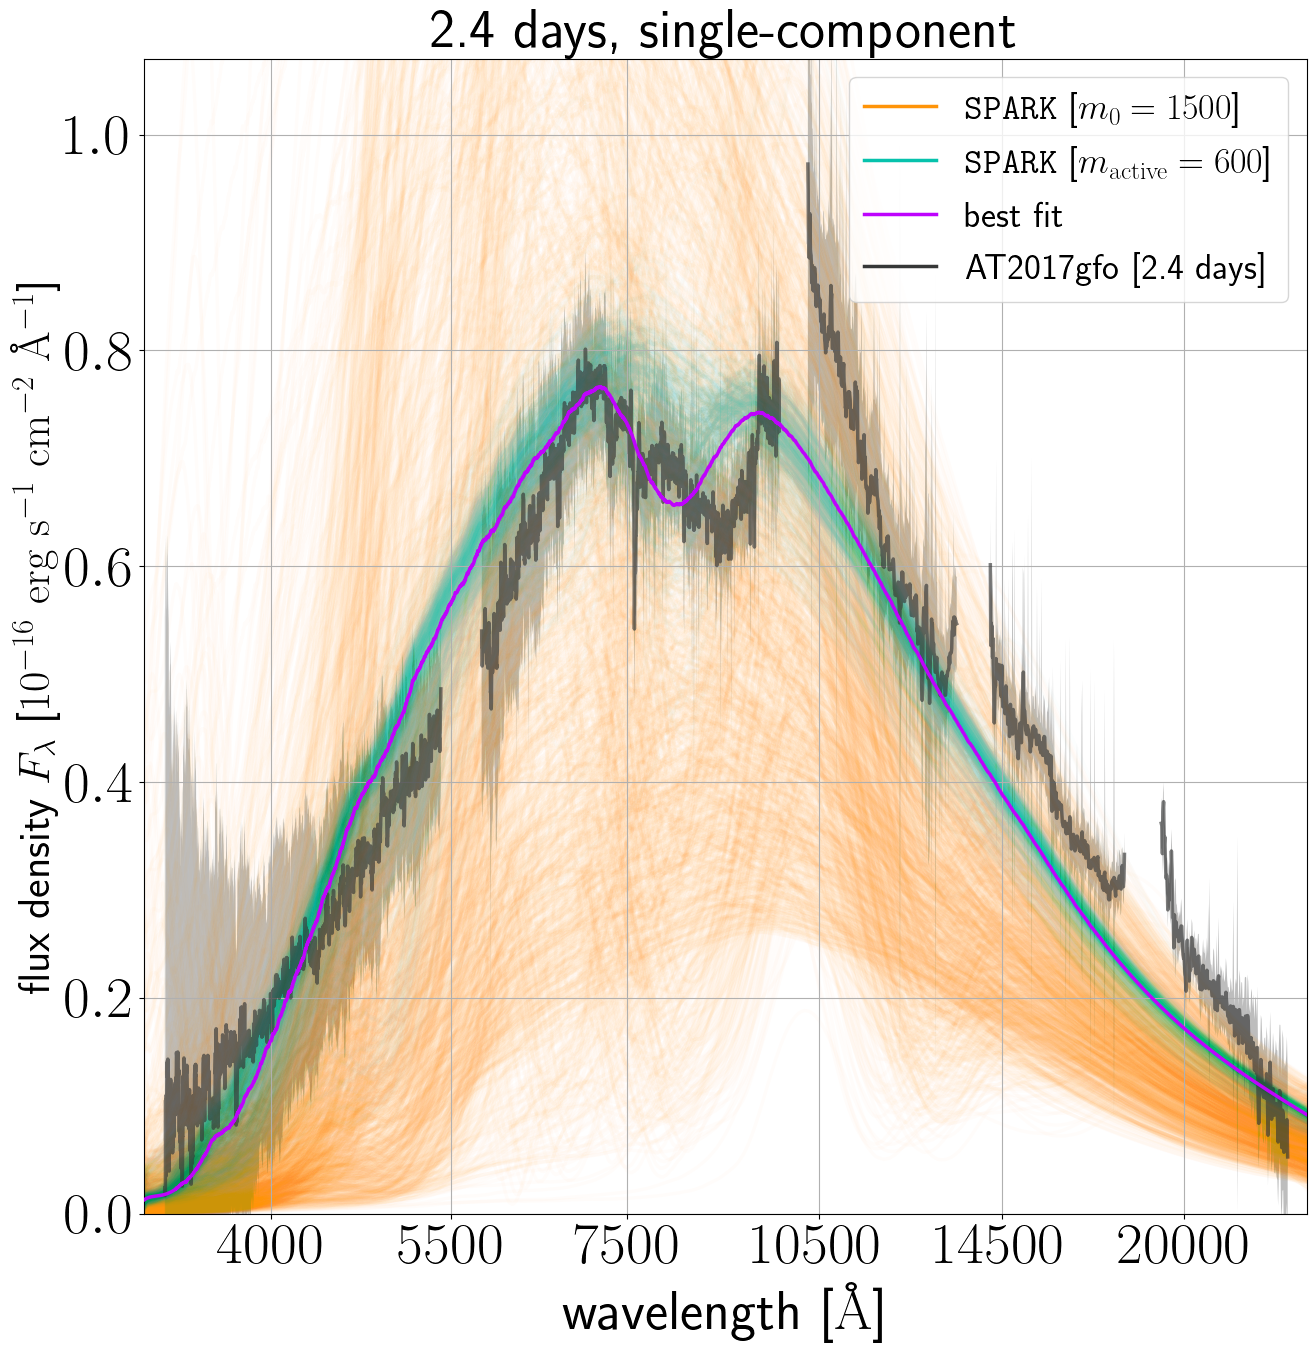
\includegraphics[width=0.47\textwidth]{figs/appendix/all-spec/221024_080947_single_all_TARDIS_evals_mactive-600_m0-1500.png}
    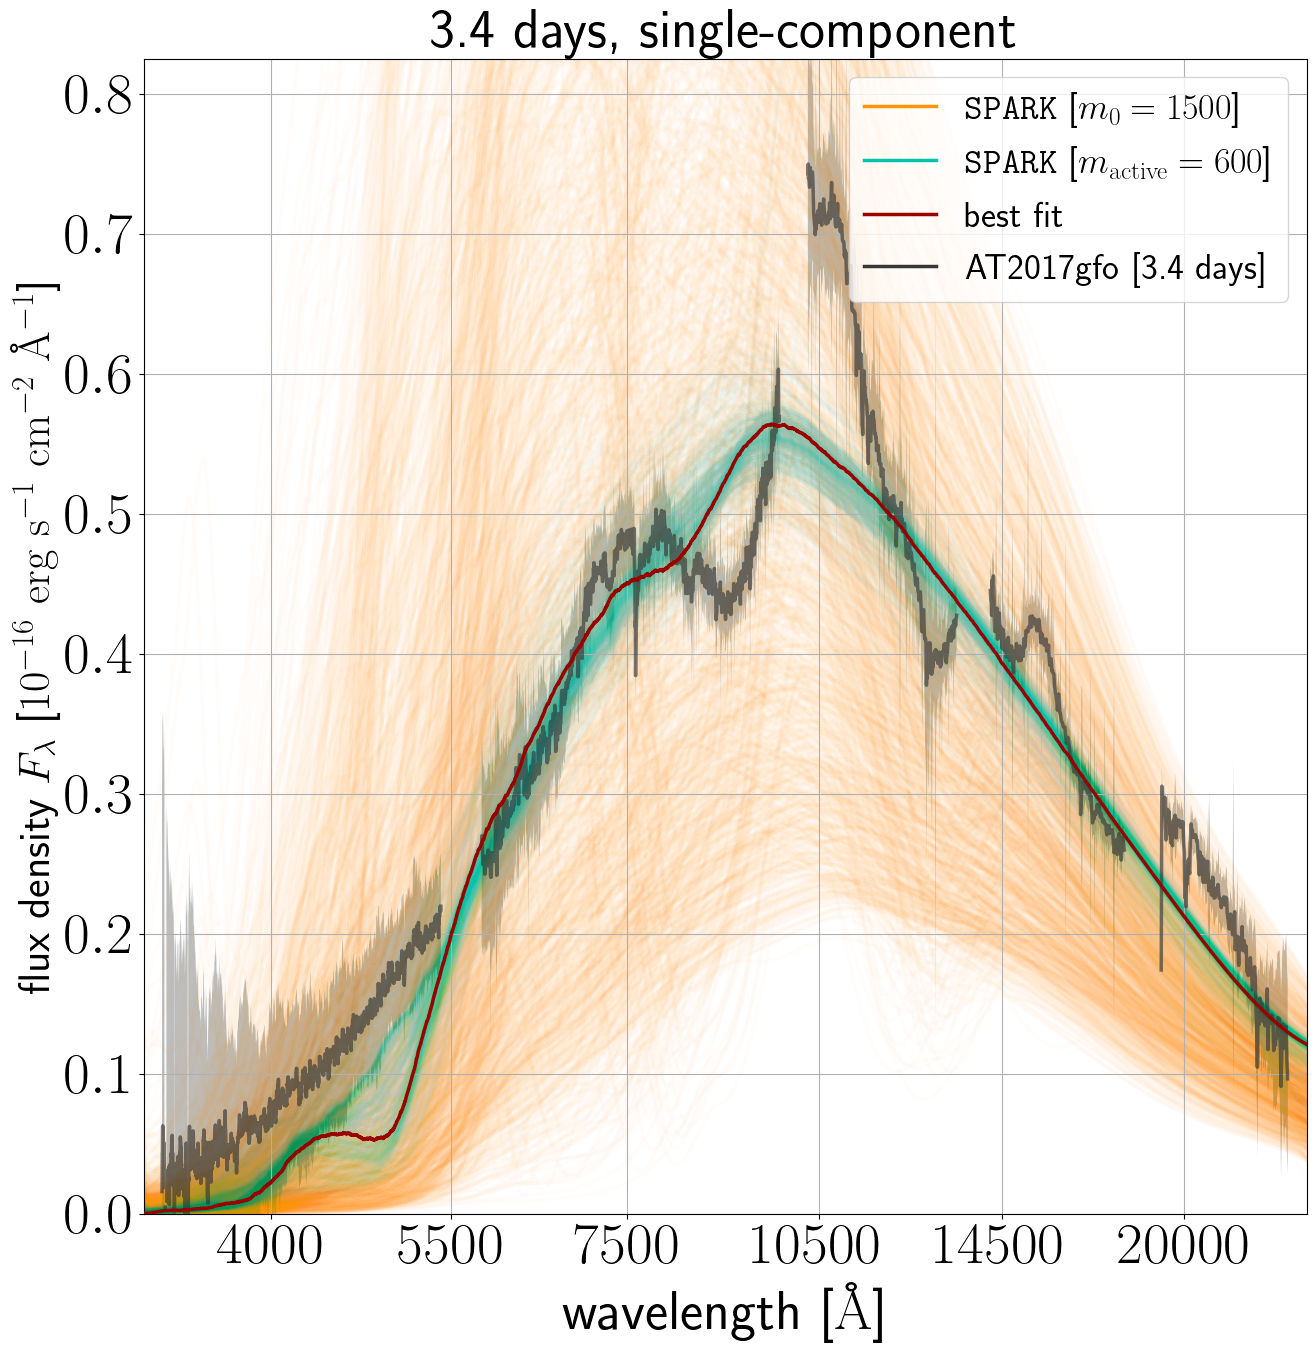
\includegraphics[width=0.47\textwidth]{figs/appendix/all-spec/230621_082134_single_all_TARDIS_evals_mactive-600_m0-1500.png}
    \figcaption{\textbf{All spectra in the training set, and the best fits, for the single-component \SPARK~runs at 2.4 and 3.4 days.} \textit{Left:} Spectra corresponding to the $m_0 = 1500$ initial Latin Hypercube samples to explore parameter space and $m_{\mathrm{active}} = 600$ additional active learning points selected using BAPE, for the fit to the 2.4 day spectrum of AT2017gfo. We also show the best fit, as obtained from the median of the posteriors. \textit{Right:} The same, for the 3.4 day fit. See Appendix~\ref{app:corners_single} for the complete posteriors for these single-component models.}\label{fig:all_spec_single}
\end{figure*}


%%% === APPENDIX B === %%%
%% ALL SPECTRA FOR MULTI-COMPONENT RUNS %%
\section{All Runs---Multi-Component Runs}\label{app:allspec_multi}

Figure~\ref{fig:all_spec_multi} shows all of the spectra used in the multi-component \SPARK~runs at 1.4, 2.4, and 3.4 days post-merger. These include the $m_0 = 1500$ Latin Hypercube Samples, $m_{\mathrm{active}}$ active learning samples, and best fit spectrum, for each.

%% all spectra
\begin{figure*}[!ht]
    \centering
    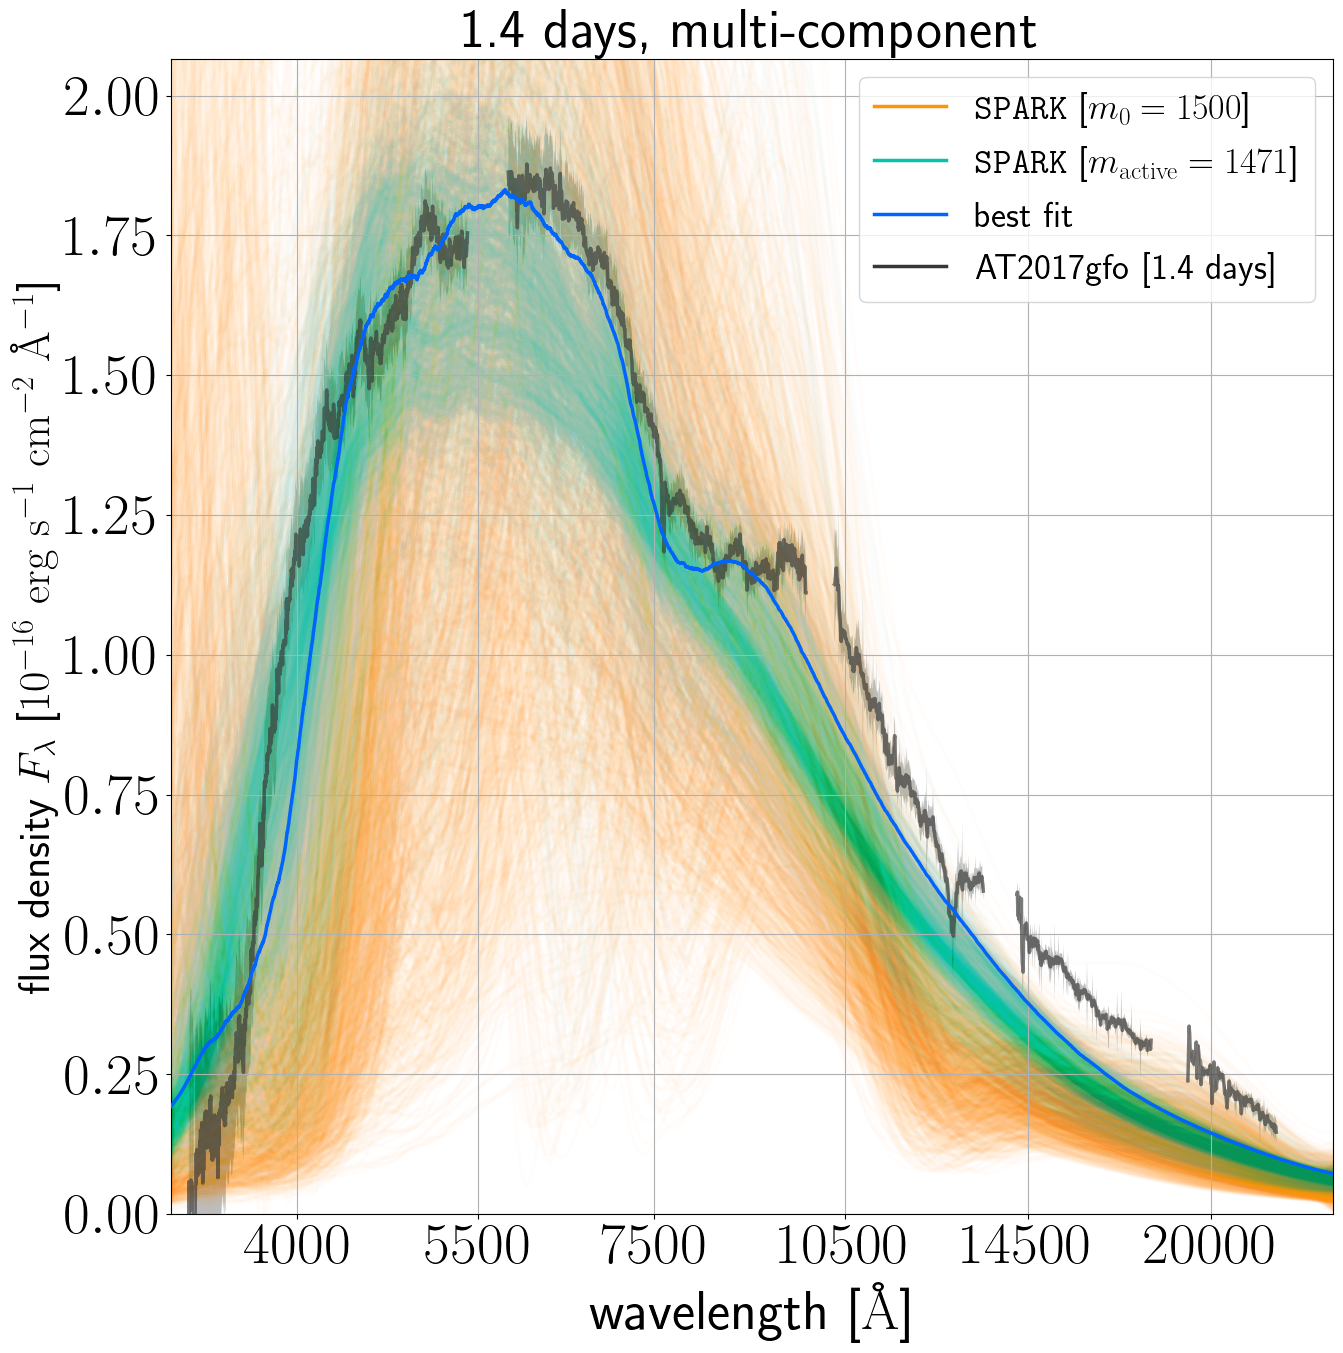
\includegraphics[width=0.47\textwidth]{figs/appendix/all-spec/230412_040127_single_all_TARDIS_evals_mactive-1471_m0-1500.png}
    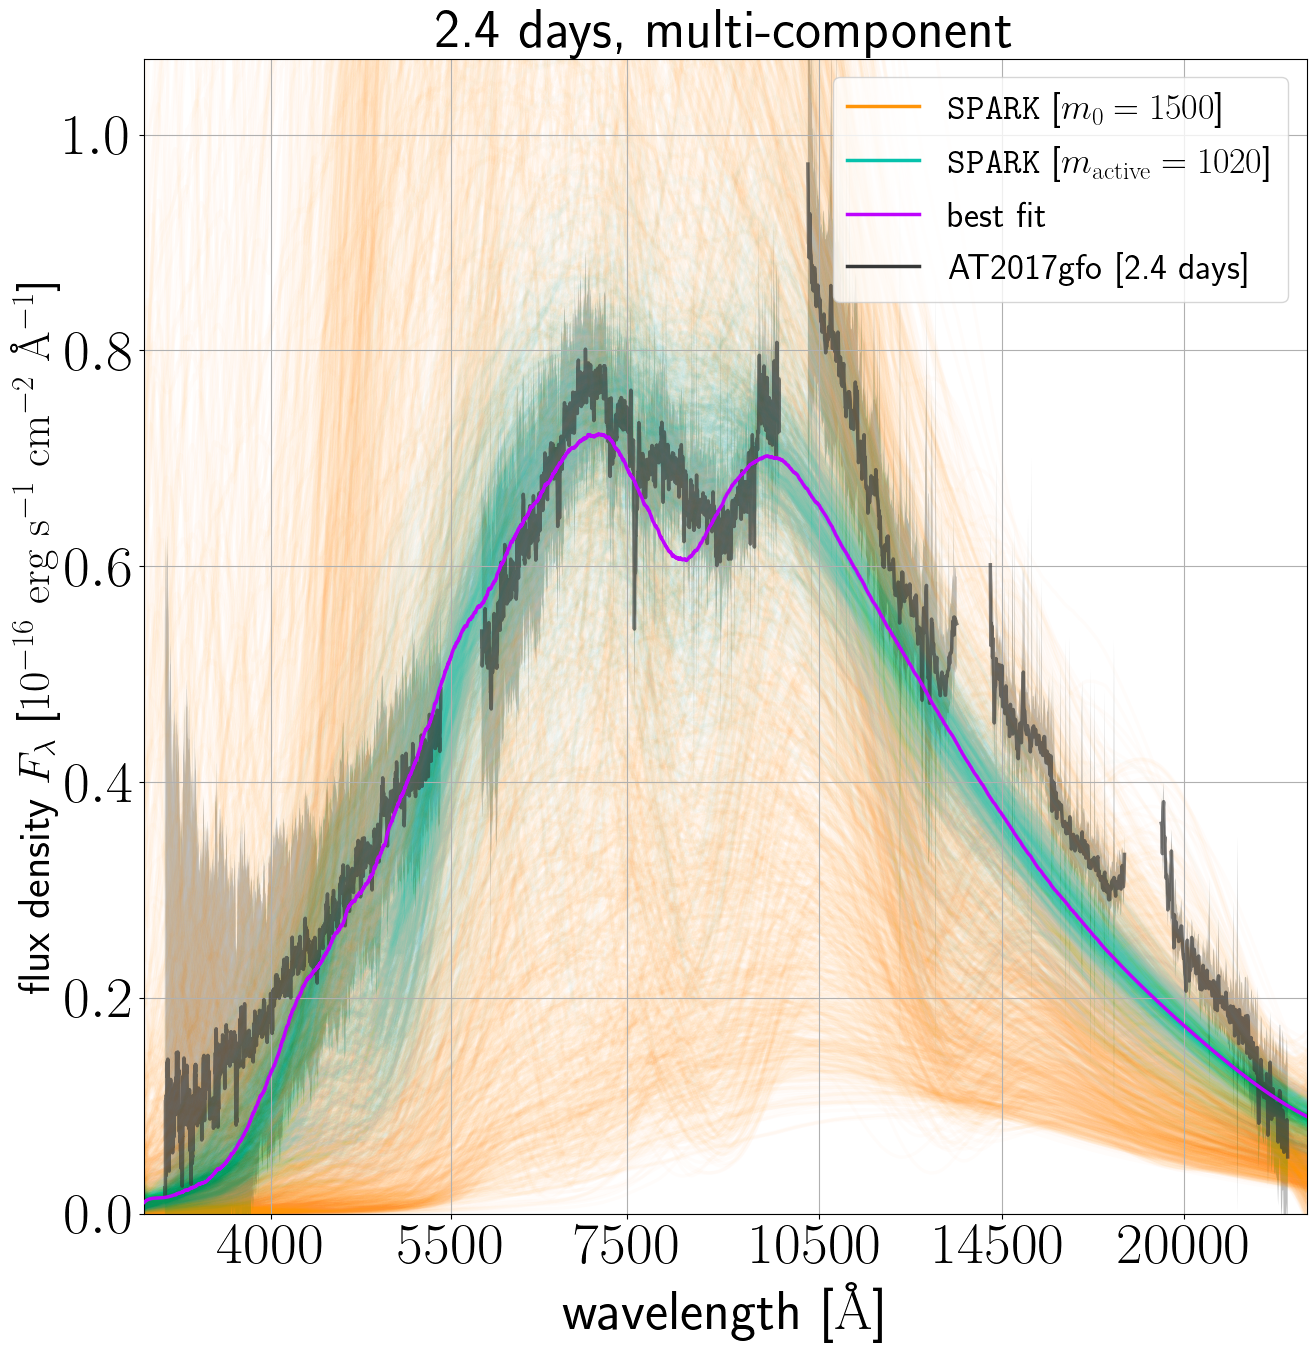
\includegraphics[width=0.47\textwidth]{figs/appendix/all-spec/230412_035244_single_all_TARDIS_evals_mactive-1020_m0-1500.png}
    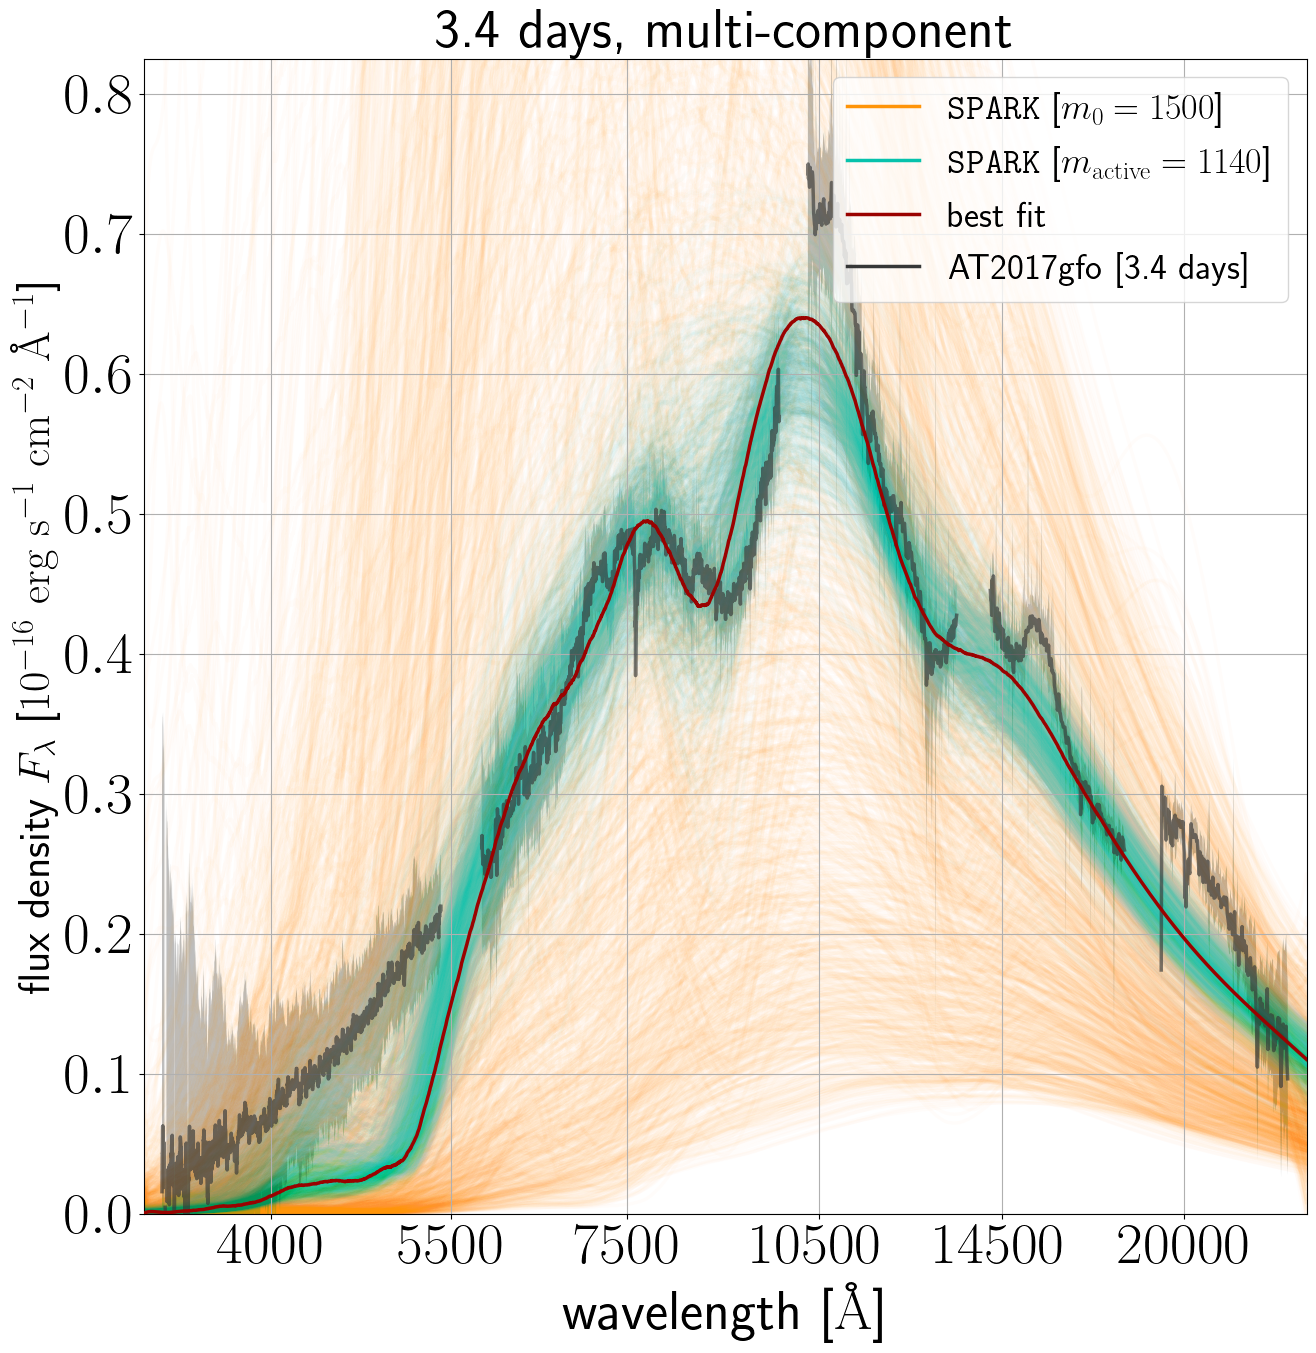
\includegraphics[width=0.47\textwidth]{figs/appendix/all-spec/230626_073230_single_all_TARDIS_evals_mactive-1140_m0-1500.png}
    \figcaption{\textbf{All spectra in the training set, and the best fits, for the multi-component \SPARK~runs at 1.4, 2.4, and 3.4 days.} \textit{Top left:} Spectra corresponding to the $m_0 = 1500$ initial Latin Hypercube samples to explore parameter space and $m_{\mathrm{active}} = 1471$ additional active learning points selected using BAPE, for the fit to the 1.4 day spectrum of AT2017gfo. We also show the best fit, as obtained from the median of the posteriors \textit{Top right:} The same, for the 2.4 day fit. $m_{\mathrm{active}} = 1020$ active learning samples are included. \textit{Bottom center:} The same for the 3.4 day fit. $m_{\mathrm{active}} = 1140$ active learning samples are included. See Appendix~\ref{app:corners_multi} for the complete posteriors for these multi-component models.}\label{fig:all_spec_multi}
\end{figure*}



%%% === APPENDIX C === %%%
%% SINGLE-COMPONENT POSTERIORS %%
\section{Posteriors---Single-component Models}\label{app:corners_single}


Figures \ref{fig:corner_single_2.4}~/~\ref{fig:corner_single_2.4_zoom} and~\ref{fig:corner_single_3.4}~/~\ref{fig:corner_single_3.4_zoom} show the full posteriors for the new single-component fits to the 2.4 and 3.4 day spectra, respectively. Both posteriors are multi-modal; we also highlight the modes which correspond to the best fits given in Table~\ref{tab:bestfit_single}. Samples from these single-component posteriors can be accessed online.\footnote{\redbf{Add a link to the posteriors? Extended data objects?}}


%% corner plots

\begin{figure*}[!ht]
    \includegraphics[width=0.95\textwidth]{figs/appendix/corners/221022_084052_dynesty_corner_pretty_smooth2d0.05_nodatapts.png}
    \figcaption{\textbf{Posterior from the single-component \SPARK~run at 2.4 days.} All posteriors are obtained through dynamic nested sampling of the surrogate Gaussian Process using \texttt{dynesty} (\citealt{speagle20}). The posterior presents some bimodality, most evident in the $s/k_{\mathrm{B}}$ dimension. In Figure~\ref{fig:corner_single_2.4_zoom}, we discard samples with $s/k_{\mathrm{B}} \geqslant 25.0$. This lower-entropy mode of the posterior is our preferred model.}\label{fig:corner_single_2.4}
\end{figure*}

\begin{figure*}[!ht]
    \includegraphics[width=0.95\textwidth]{figs/appendix/corners/221022_084052_dynesty_corner_pretty_smooth2d0.05_nodatapts_zoom.png}
    \figcaption{\textbf{Posterior from the single-component \SPARK~run at 2.4 days, zoomed in to the mode which produces the best fit.} Samples $s/k_{\mathrm{B}} \geqslant 25.0$ are discarded to show only the mode of the posterior which corresponds to the preferred model in Table~\ref{tab:bestfit_single}.}\label{fig:corner_single_2.4_zoom}
\end{figure*}


\begin{figure*}[!ht]
    \includegraphics[width=0.95\textwidth]{figs/appendix/corners/230618_143307_dynesty_corner_pretty_mactive-600_smooth2d0.05_nodatapts.png}
    \figcaption{\textbf{Posterior from the single-component \SPARK~run at 3.4 days.} The posterior at this epoch is highly multi-modal, as most evident in the $\rho_0,~Y_{\mathrm{e}},~\mathrm{and}~s/k_{\mathrm{B}}$ dimensions. Although none of these modes in the posterior correspond to a good fit, and the multi-component model is favored at 3.4 days, we find the higher-$\rho_0$, mid-$Y_{\mathrm{e}}$, low-$s$ mode produces the best possible fit with single-component ejecta. In Figure~\ref{fig:corner_single_3.4_zoom}, we highlight this mode of the posterior by discarding samples outside the range $\log_{10}(\rho_0 / \mathrm{g~cm^{-3}}) \in [-15.0, -14.0] \cup Y_{\mathrm{e}} \in [0.13, 0.29] \cup s/k_{\mathrm{B}} \in [10.0, 25.0]$.  }\label{fig:corner_single_3.4}
\end{figure*}


\begin{figure*}[!ht]
    \includegraphics[width=0.95\textwidth]{figs/appendix/corners/230618_143307_dynesty_corner_pretty_mactive-600_smooth2d0.05_nodatapts_zoom-midYe-lows-highdens_add-nlive-30000.png}
    \figcaption{\textbf{Posterior from the single-component \SPARK~run at 3.4 days, zoomed in to the mode which produces the best fit.} Samples outside the range $\log_{10}(\rho_0 / \mathrm{g~cm^{-3}}) \in [-15.0, -14.0] \cup Y_{\mathrm{e}} \in [0.13, 0.29] \cup s/k_{\mathrm{B}} \in [10.0, 25.0]$ are discarded to show only the mode of the posterior which corresponds to the preferred model in Table~\ref{tab:bestfit_single}.}\label{fig:corner_single_3.4_zoom}
\end{figure*}



%%% === APPENDIX D === %%%
%% MULTI-COMPONENT POSTERIORS %%
\section{Posteriors---Multi-component Models}\label{app:corners_multi}

Figures~\ref{fig:corner_multi_1.4},~\ref{fig:corner_multi_2.4}, and~\ref{fig:corner_multi_3.4} show the full posteriors for the new multi-component fits to the 1.4, 2.4, and 3.4 day spectra, respectively. Samples from these multi-component posteriors can be accessed online.\footnote{\redbf{Add a link to the posteriors? Extended data objects?}}


%% corner plots
\begin{figure*}[!ht]
    \includegraphics[width=0.95\textwidth]{figs/appendix/corners/230103_064024_dynesty_corner_pretty_mactive-1471_smooth2d0.05_nodatapts.png}
    \figcaption{\textbf{Posterior from the multi-component \SPARK~run at 1.4 days.} The posterior contains one lower-probability mode, most evident in the $\log_{10}(\rho_0 / \mathrm{g~cm^{-3}}$ and $v_{\mathrm{inner},1}$ dimensions. We ignore this mode, as the median of the higher-probability mode yields our best fit, as given in Table~\ref{tab:bestfit_multi}.}\label{fig:corner_multi_1.4}
\end{figure*}

\begin{figure*}[!ht]
    \includegraphics[width=0.95\textwidth]{figs/appendix/corners/230103_060017_dynesty_corner_pretty_mactive-1020_smooth2d0.05_nodatapts.png}
    \figcaption{\textbf{Posterior from the multi-component \SPARK~run at 2.4 days.} As at 1.4 and 3.4 days, the posterior contains one lower-probability mode, most evident in the $v_{\mathrm{inner},1}$ dimension. We once again ignore this mode, as the median of the higher-probability mode yields our best fit, as given in Table~\ref{tab:bestfit_multi}.}\label{fig:corner_multi_2.4}
\end{figure*}

\begin{figure*}[!ht]
    \includegraphics[width=0.95\textwidth]{figs/appendix/corners/230622_230103_dynesty_corner_pretty_mactive-1140_smooth2d0.05_nodatapts}
    \figcaption{\textbf{Posterior from the multi-component \SPARK~run at 3.4 days.} As at 1.4 and 2.4 days, the posterior contains one lower-probability mode, most evident in the $v_{\mathrm{inner},1}$ dimension. We once again ignore this mode, as the median of the higher-probability mode yields our best fit, as given in Table~\ref{tab:bestfit_multi}.}\label{fig:corner_multi_3.4}
\end{figure*}


%%% === APPENDIX E === %%%
%% LEAVE-ONE-OUT SPECTRA %%
\section{Leave-one-out Spectra---Non-Preferred Models}\label{app:leave_out_multi}

In Figure~\ref{fig:leave_out_nonpref}, we show leave-one-out spectra for the non-preferred fits: multi-component for 1.4 and 2.4 days, and single-component for 3.4 days.

%% leave-one-out spectra
\begin{figure*}[!ht]
    \centering
    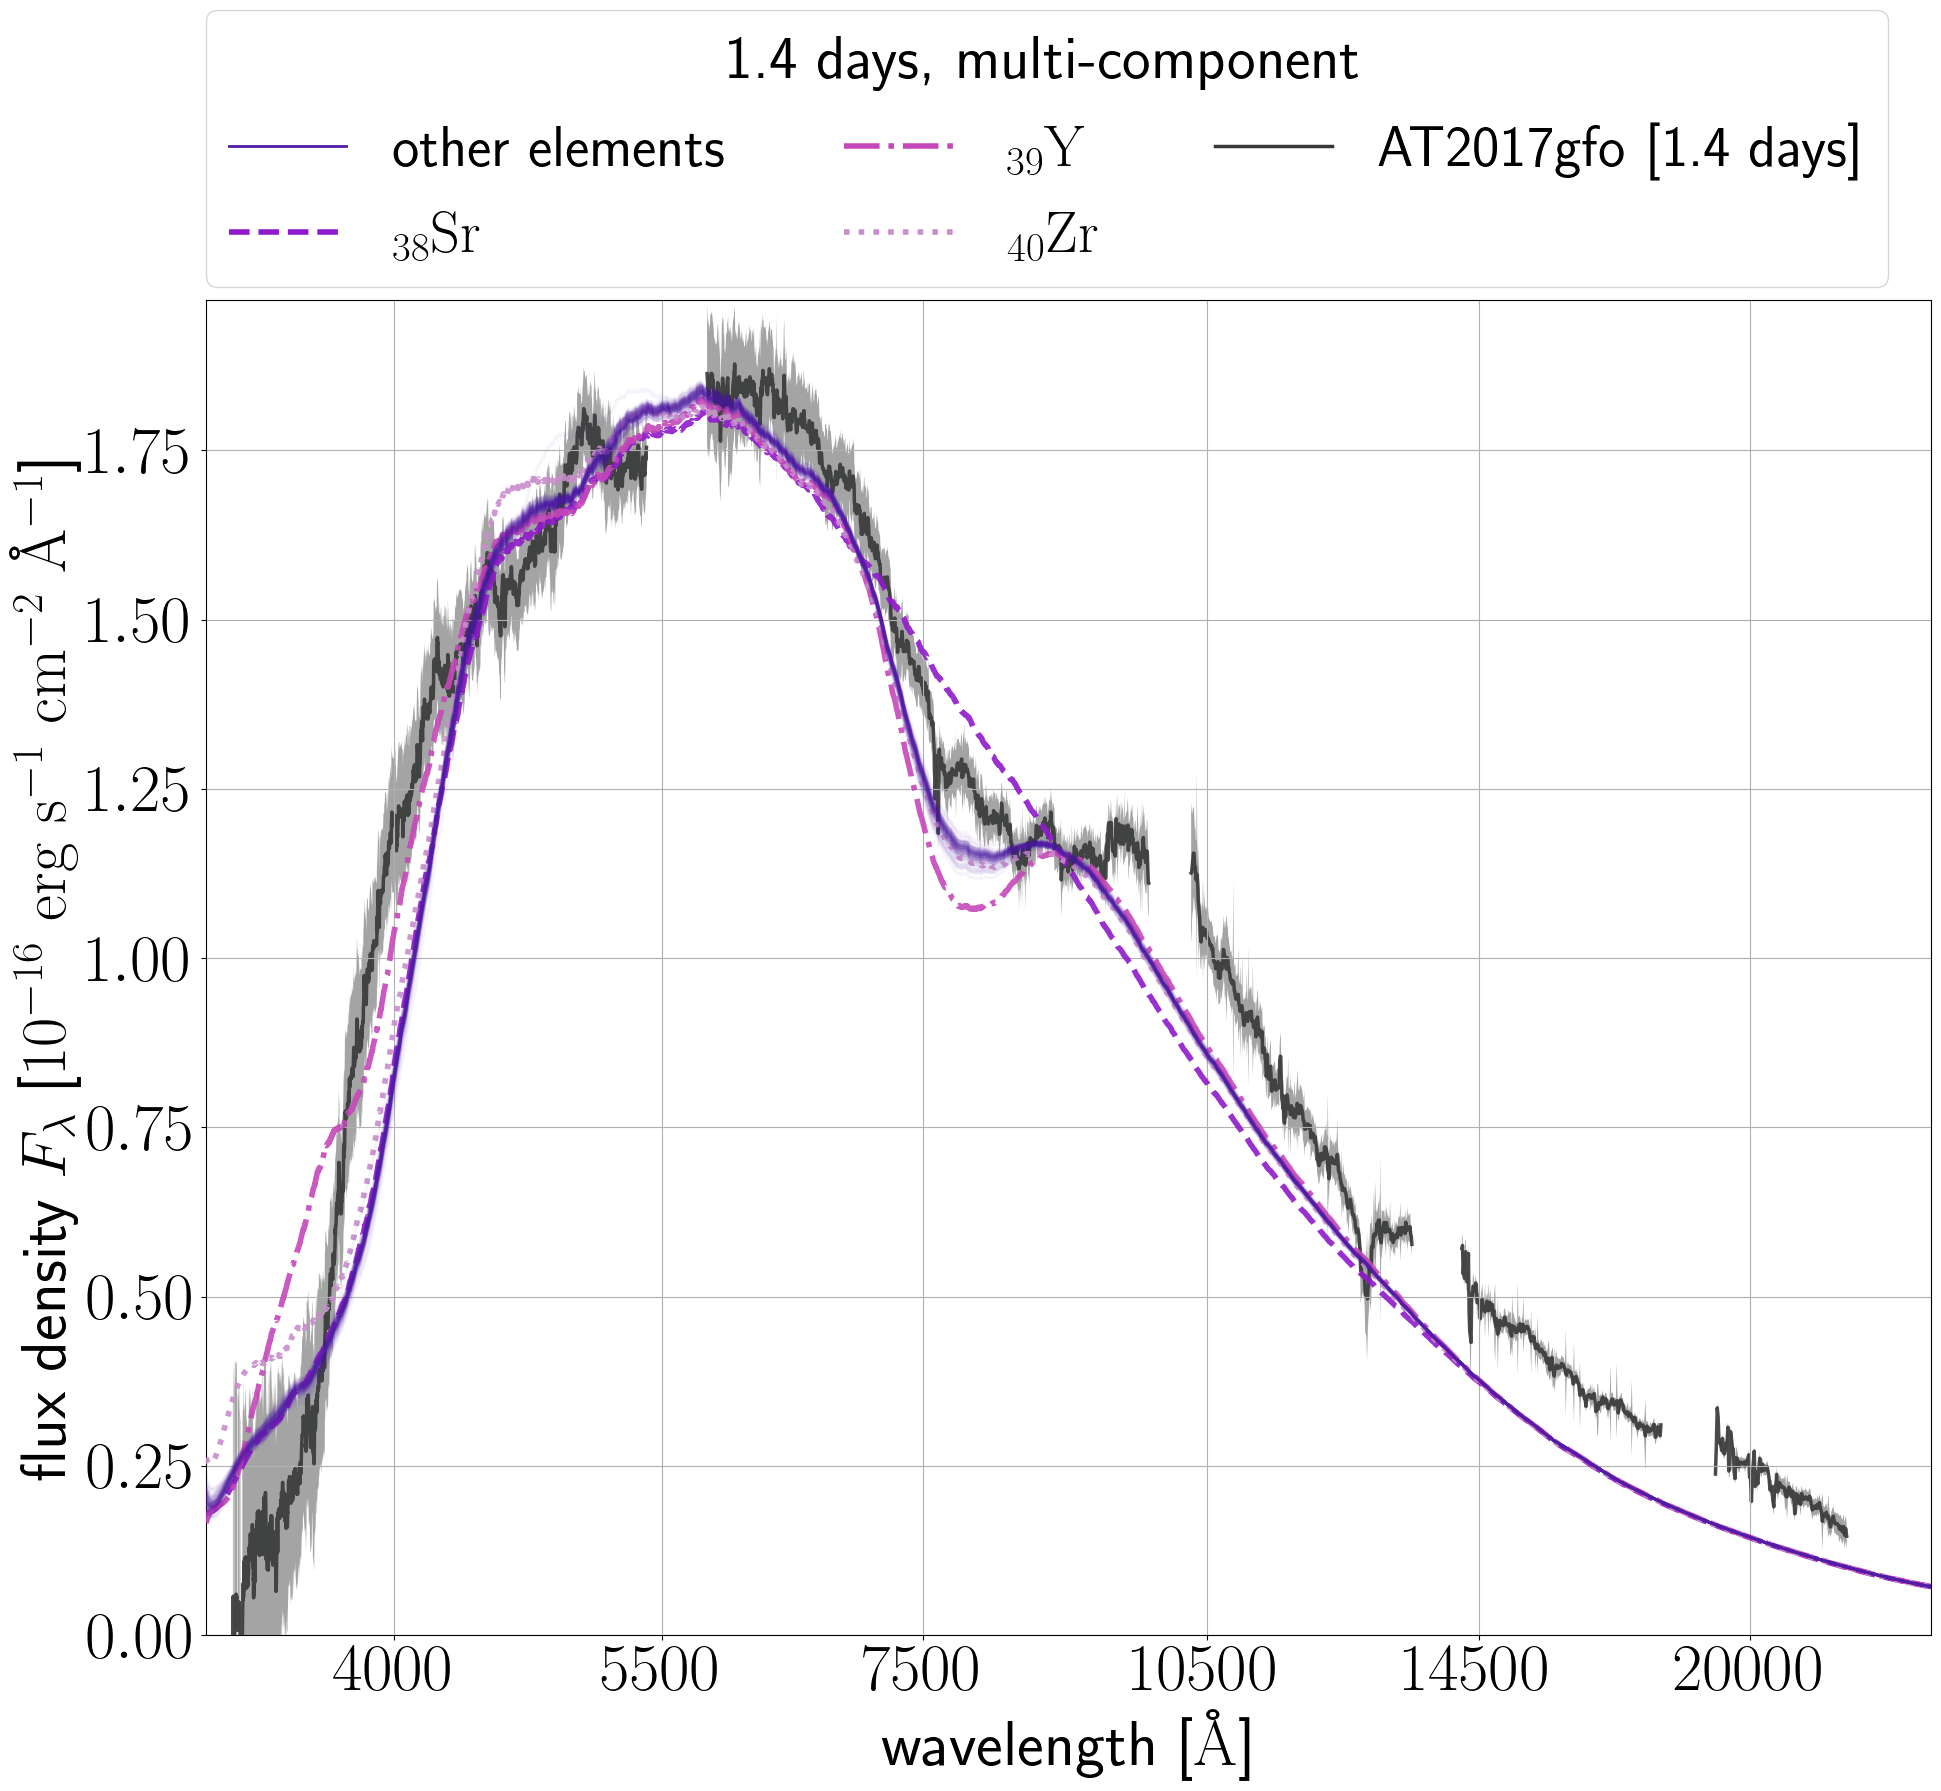
\includegraphics[width=0.47\textwidth]{figs/appendix/LoO/230503_184337_leaveoneout_all_TARDIS_evals_label-interest-38-39-40.png}
    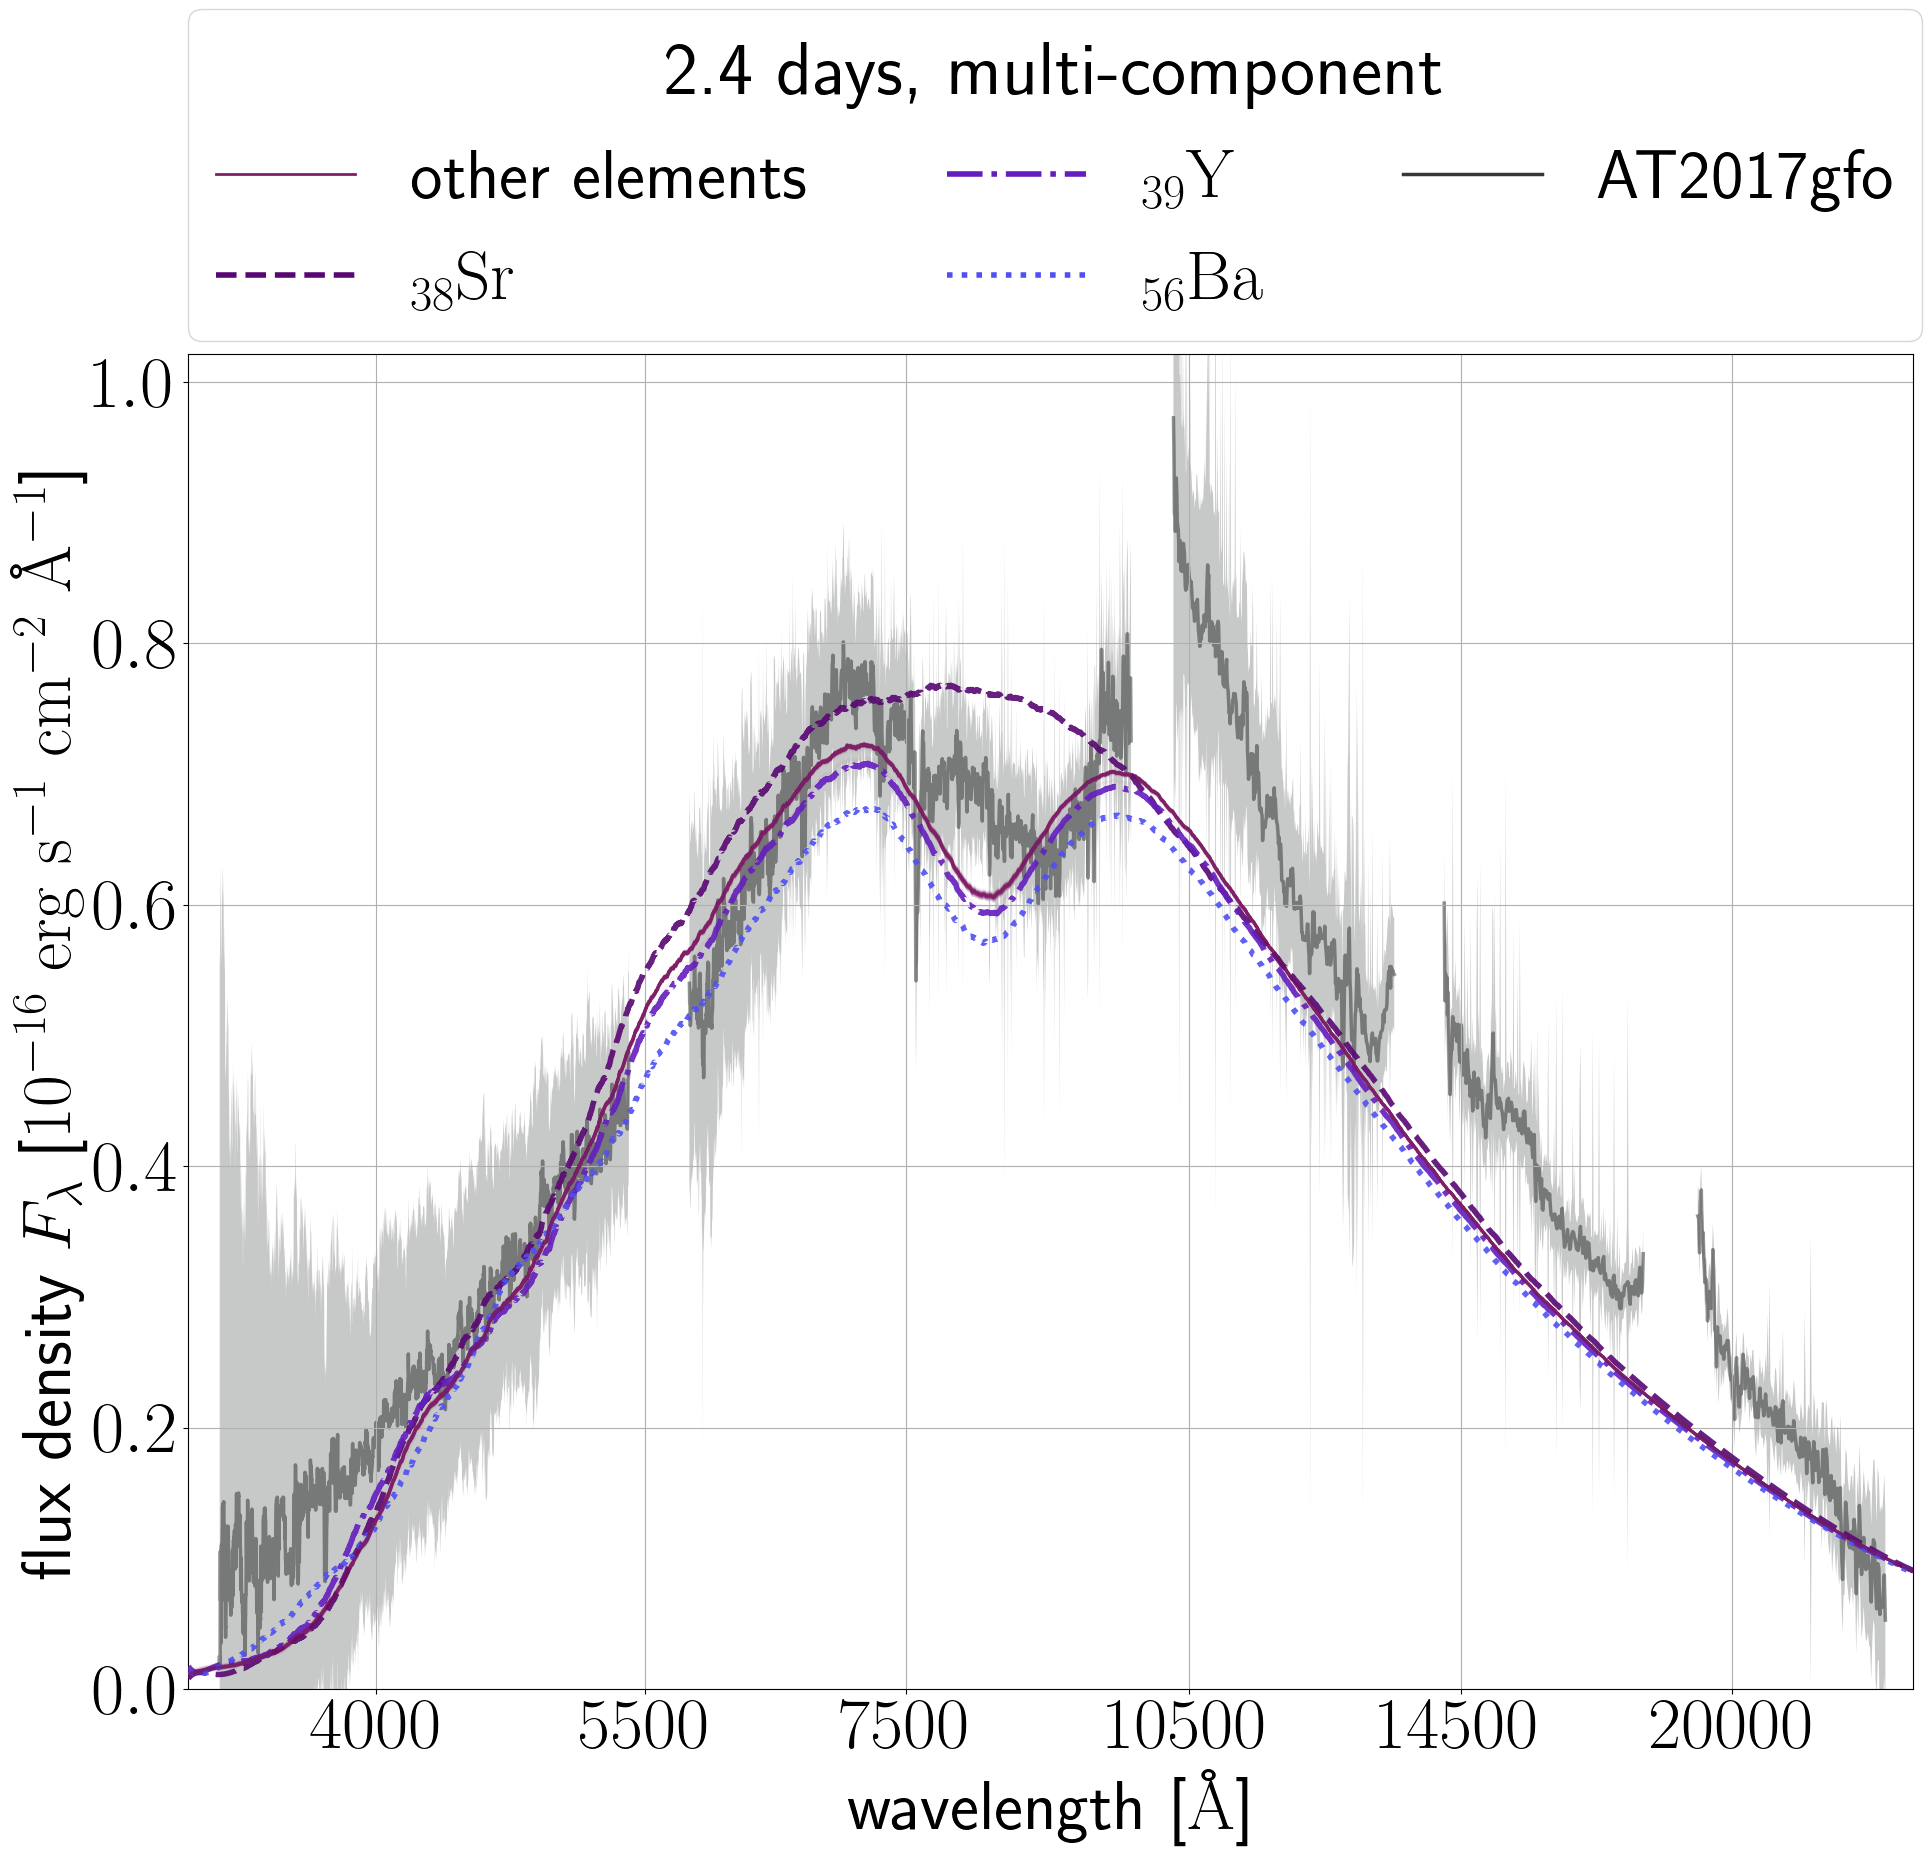
\includegraphics[width=0.47\textwidth]{figs/appendix/LoO/230504_003423_leaveoneout_all_TARDIS_evals_label-interest-38-39-56.png}
    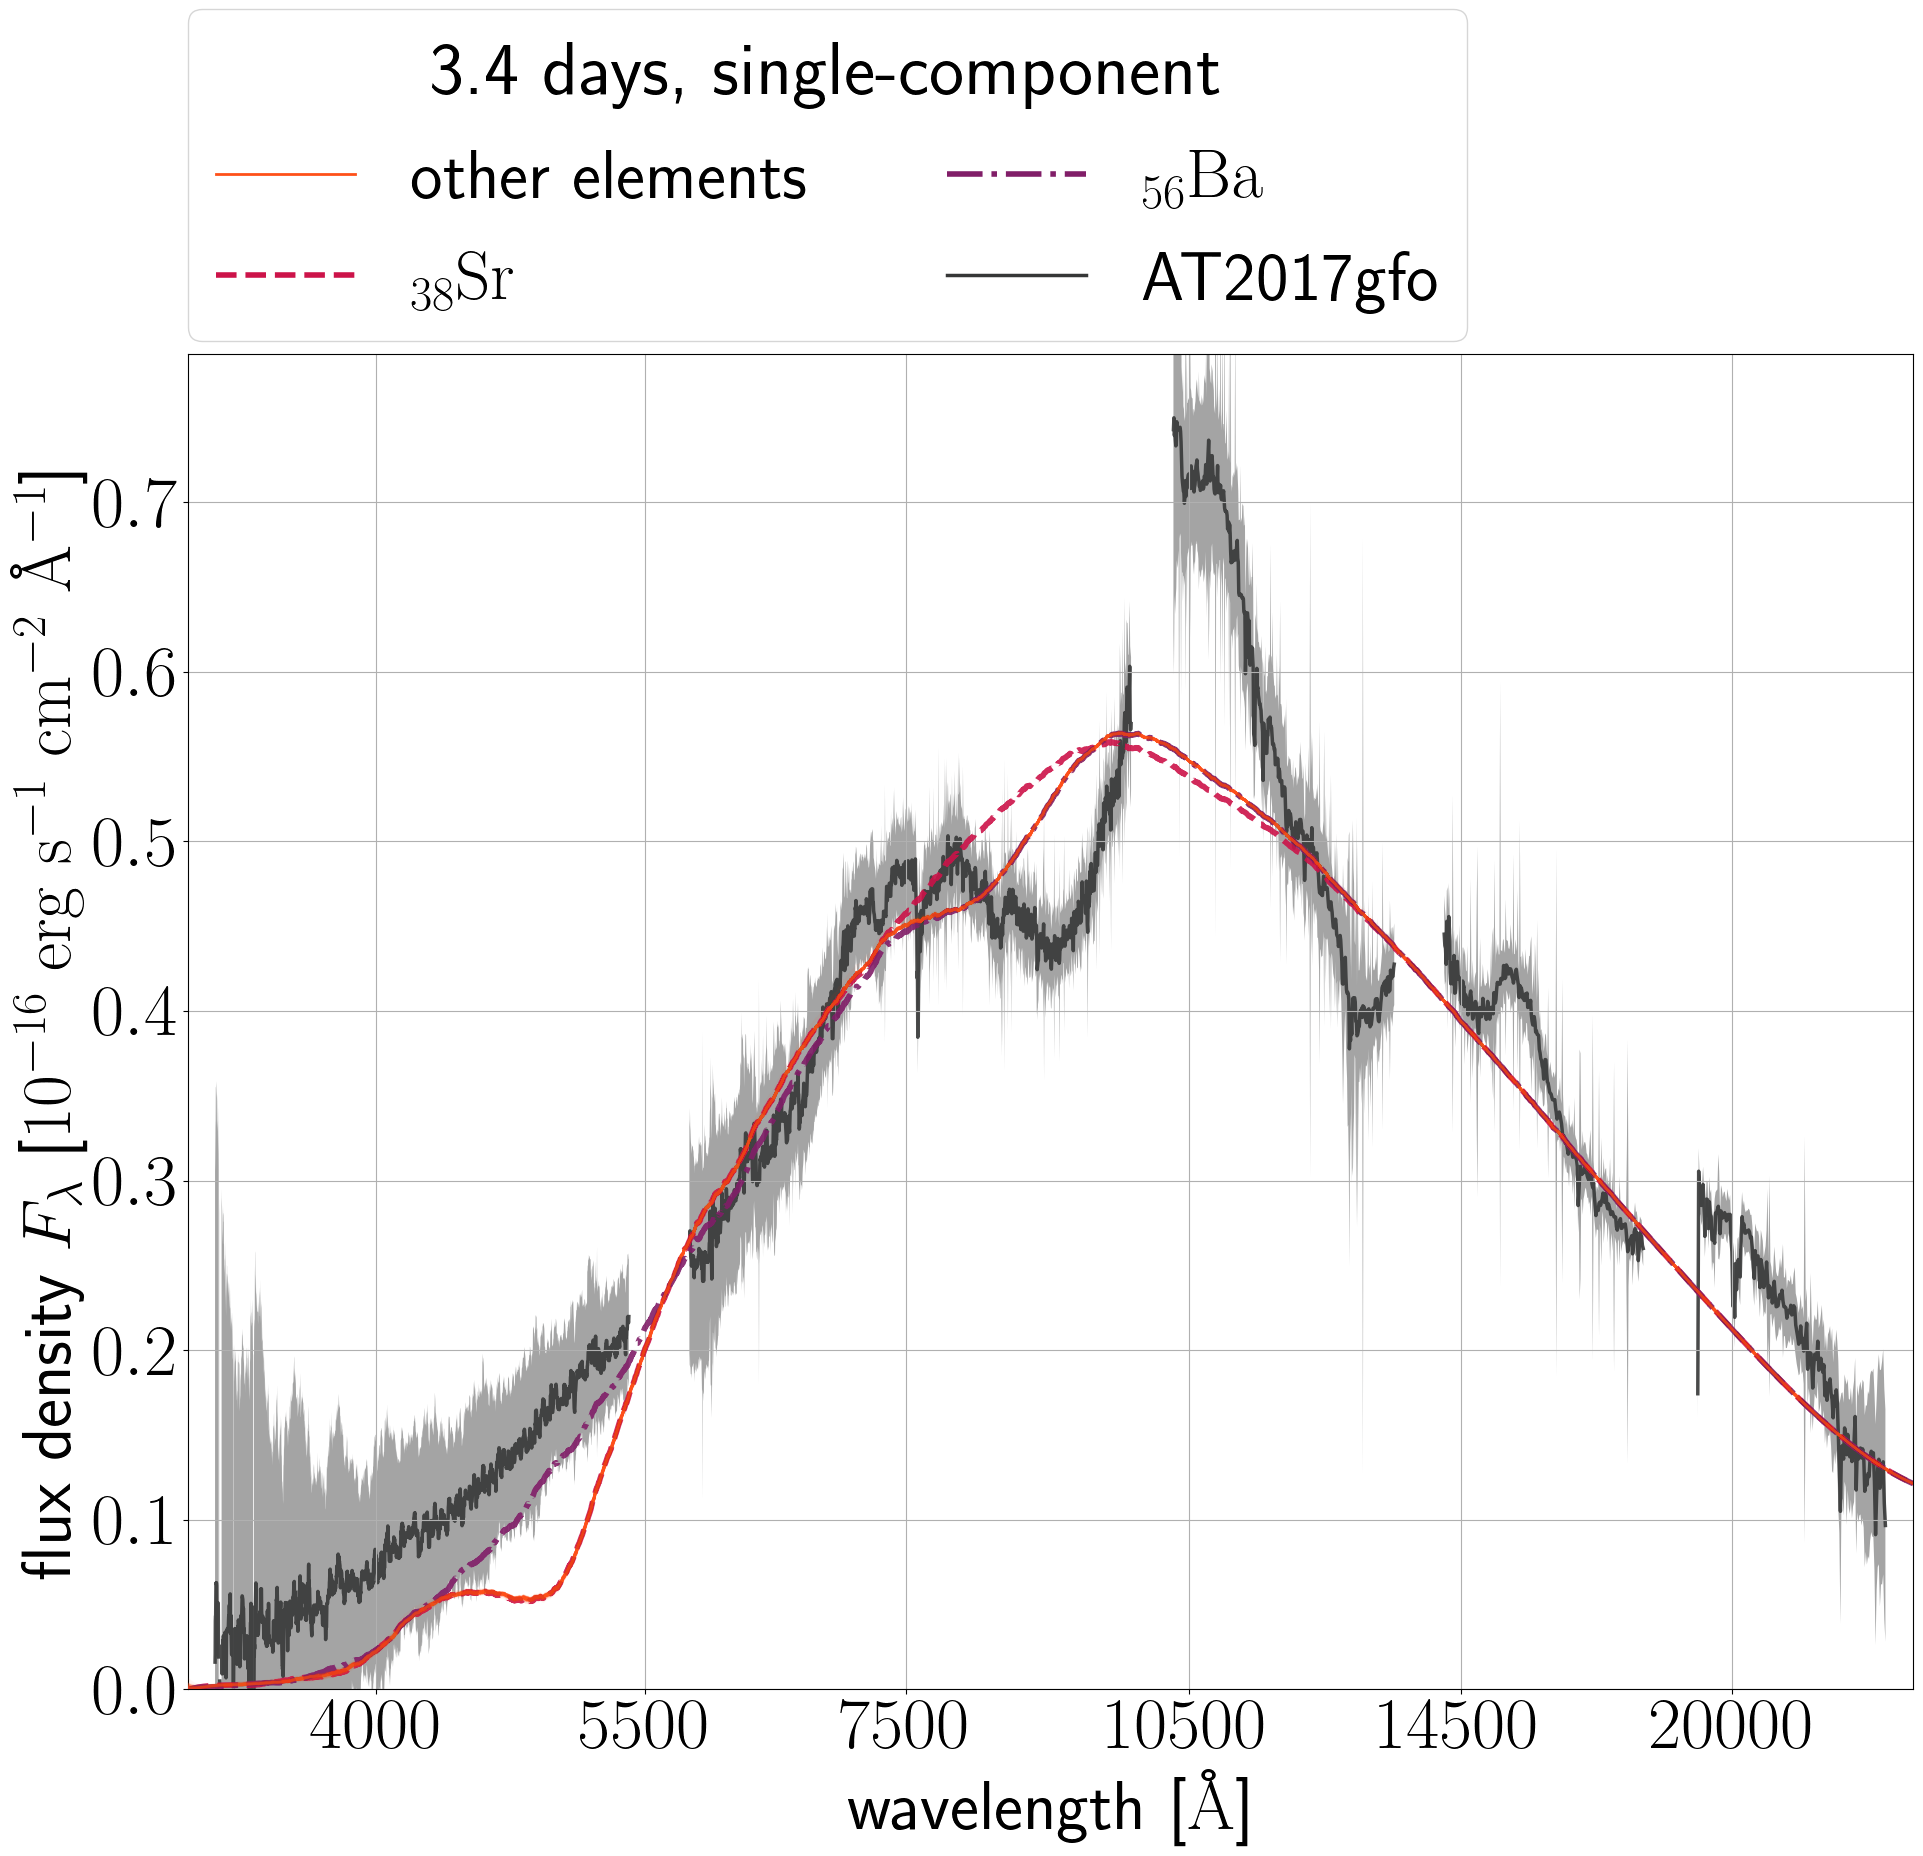
\includegraphics[width=0.47\textwidth]{figs/appendix/LoO/230628_205804_leaveoneout_all_TARDIS_evals_label-interest-38-56.png}
    \figcaption{\textbf{Leave-one-out spectra for the disfavored models: multi-component for 1.4 and 2.4 days, and single-component for 3.4 days.} All models show clear absorption from strontium (${}_{38}$Sr) at $\sim8000$\AA. Both 1.4 and 2.4 day multi-component models also show absorption from yttrium (${}_{39}$Y). At (multi-component) 2.4 and (single-component) 3.4 days, absorption from barium (${}_{56}$Ba) is also present. Spectral DEComposition (SDEC) plots, included in Appendix~\ref{app:SDEC}, provide a complementary view of the dominant species to these leave-one-out plots.}\label{fig:leave_out_nonpref}
\end{figure*}


%%% === APPENDIX F === %%%
%% SDEC %%
\section{Spectral DEComposition Spectra}\label{app:SDEC}

Figure~\ref{fig:SDEC} shows the Spectral DEComposition (SDEC) plots for all 1.4, 2.4, and 3.4 day single- and multi-component fits. These SDEC plots show the species (elements or ions) which dominate the absorption (measured by absorbed luminosity, $\mathrm{erg~s^{-1}}$) in the spectrum. These are complementary to the leave-one-out plots, which show which elements have the largest impact on the shape of the spectrum, in terms of either absorption or emission.

%% leave-one-out spectra
\begin{figure*}[!ht]
    \centering
    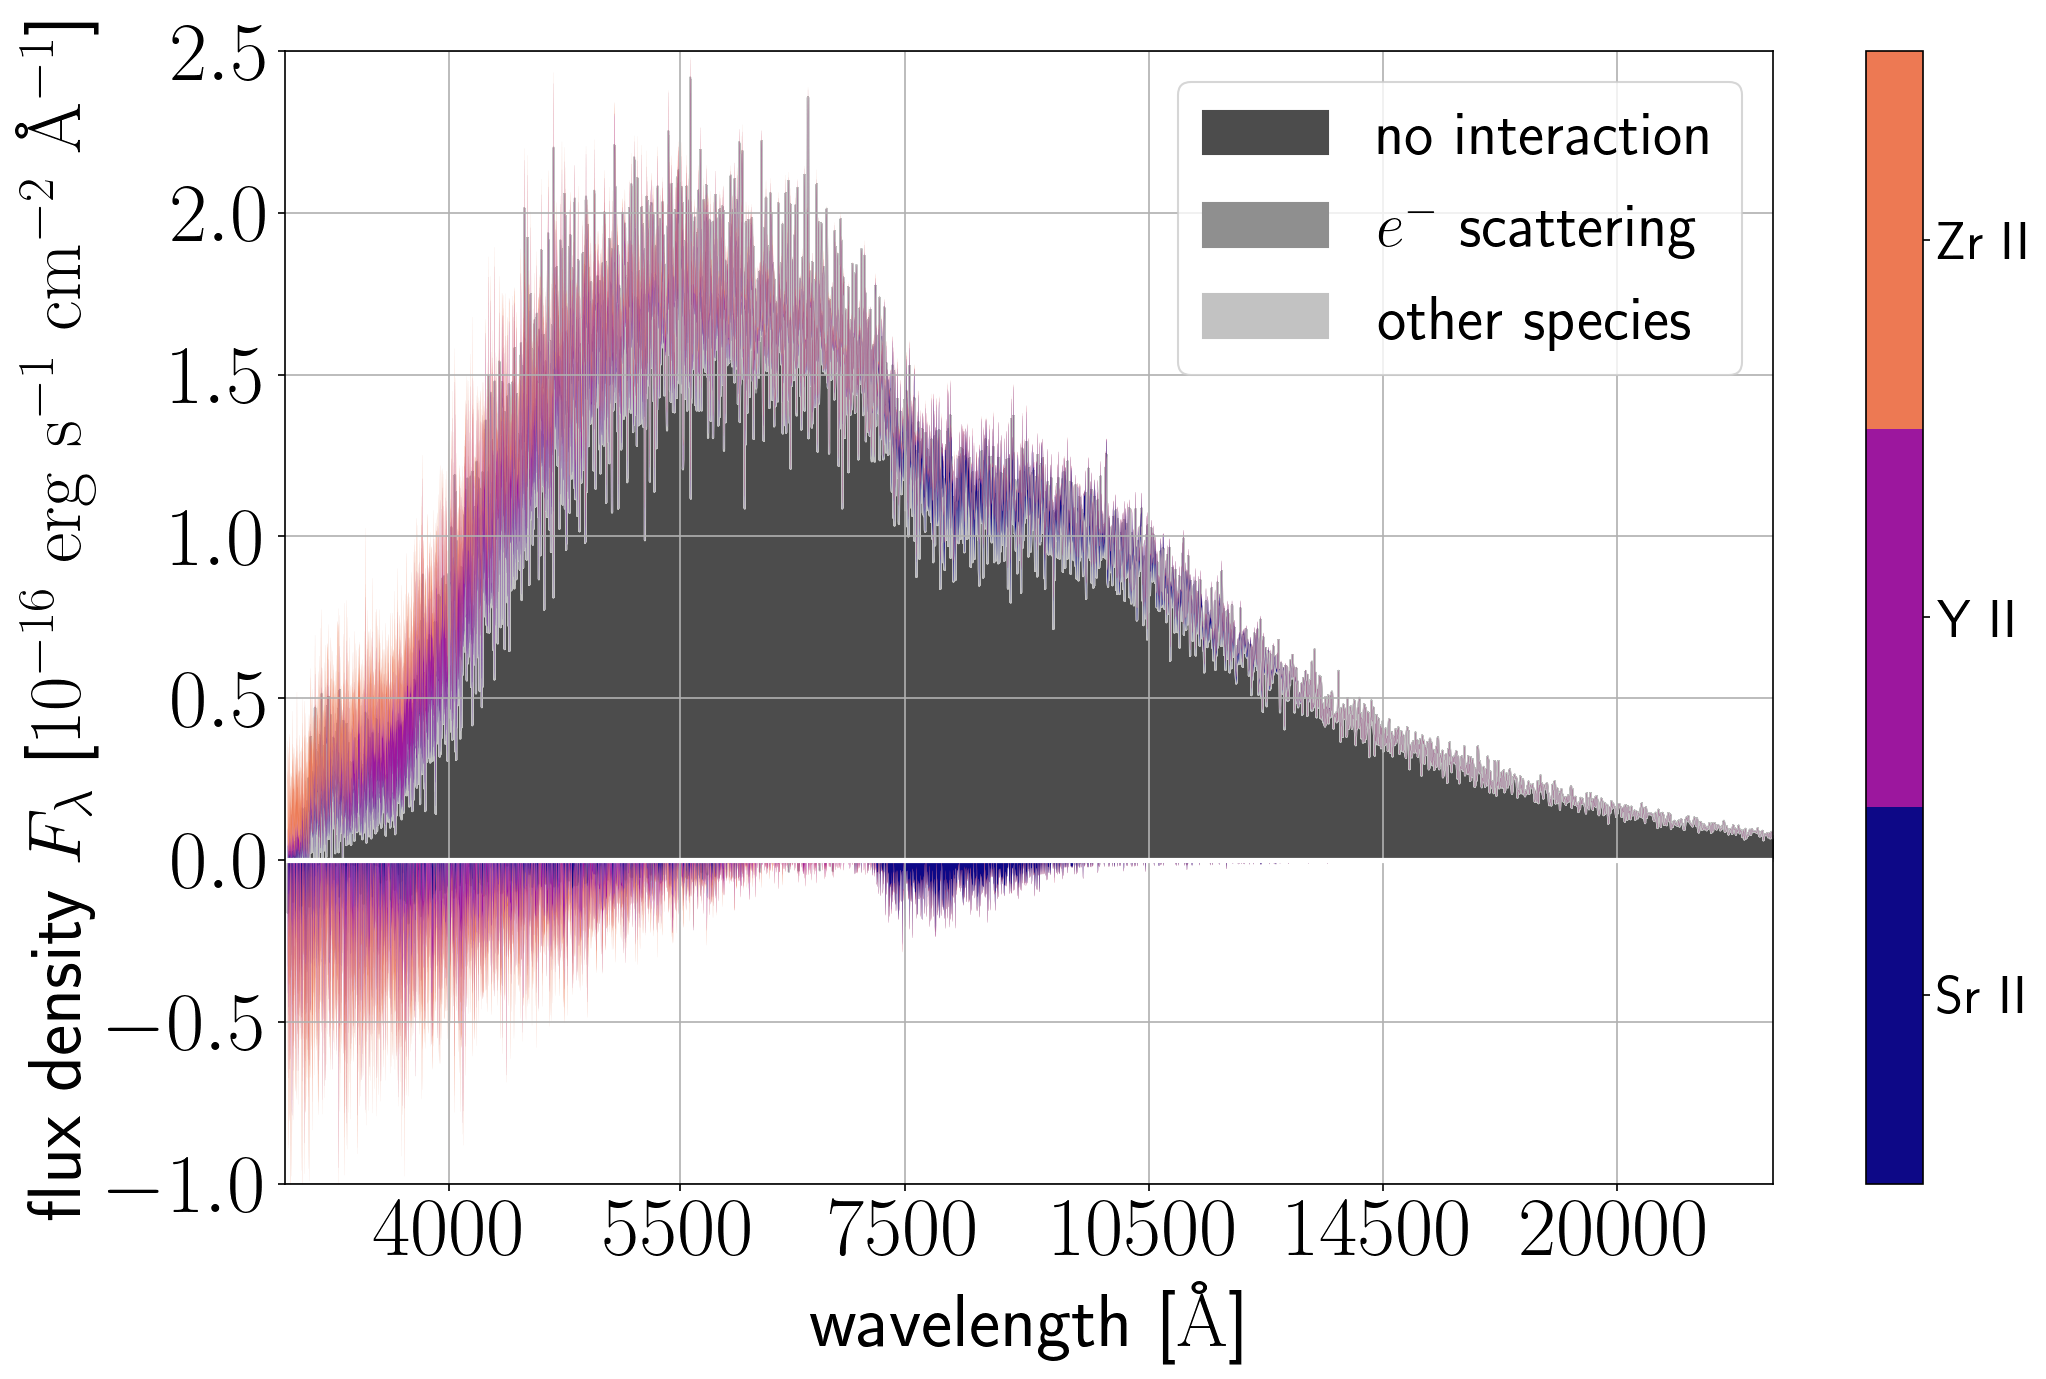
\includegraphics[width=0.47\textwidth]{figs/appendix/SDEC/230704_165812_single_TARDIS_eval_SDEC.png}
    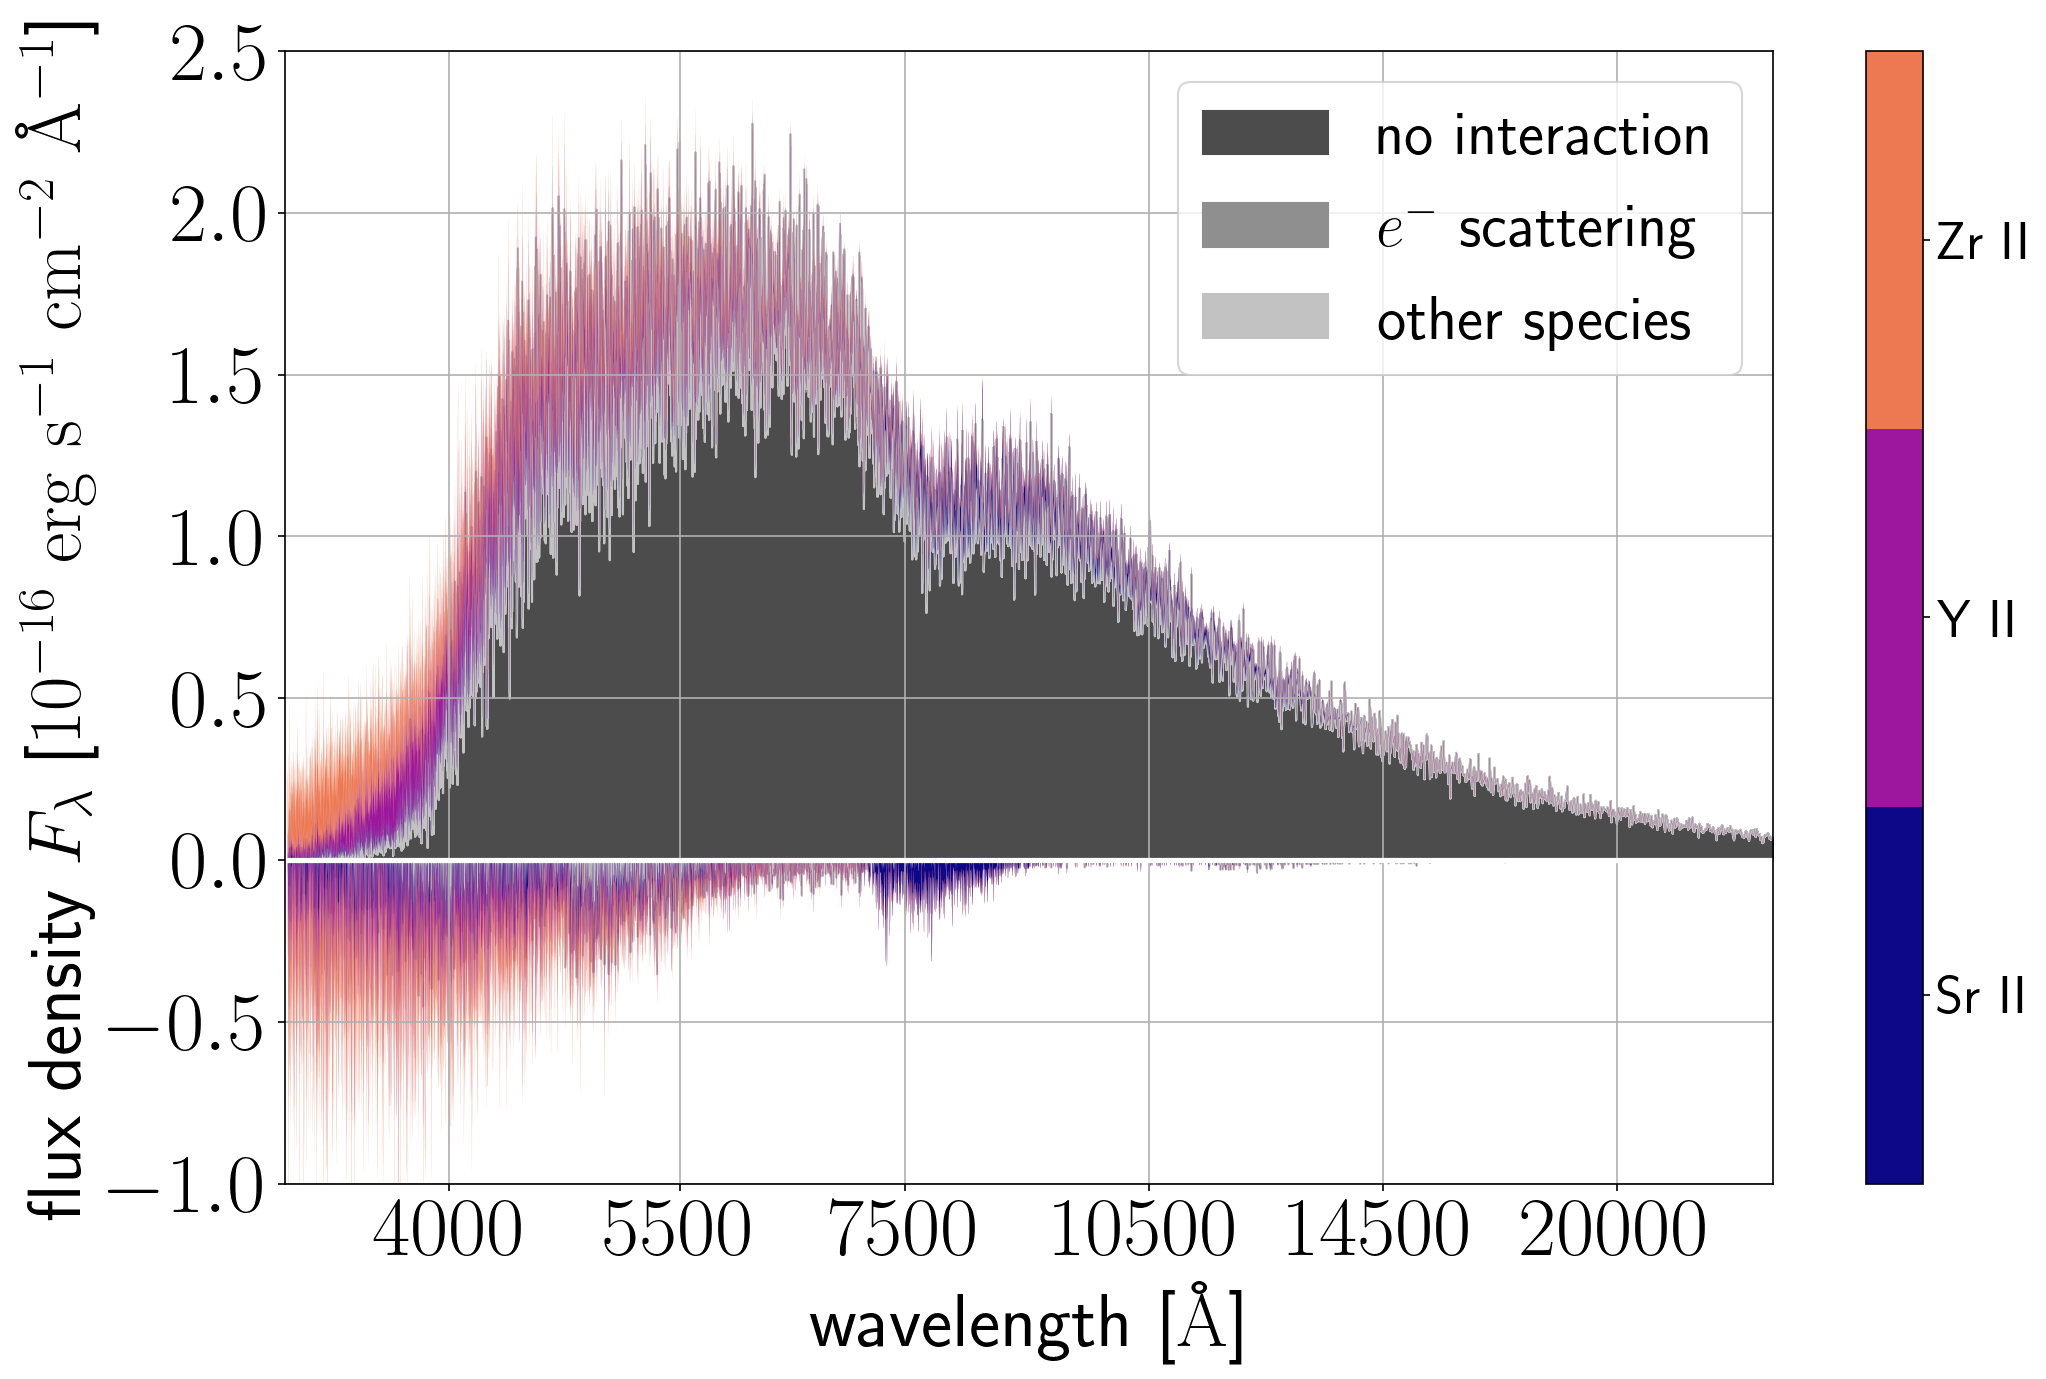
\includegraphics[width=0.47\textwidth]{figs/appendix/SDEC/230412_040127_single_TARDIS_eval_SDEC.png}
    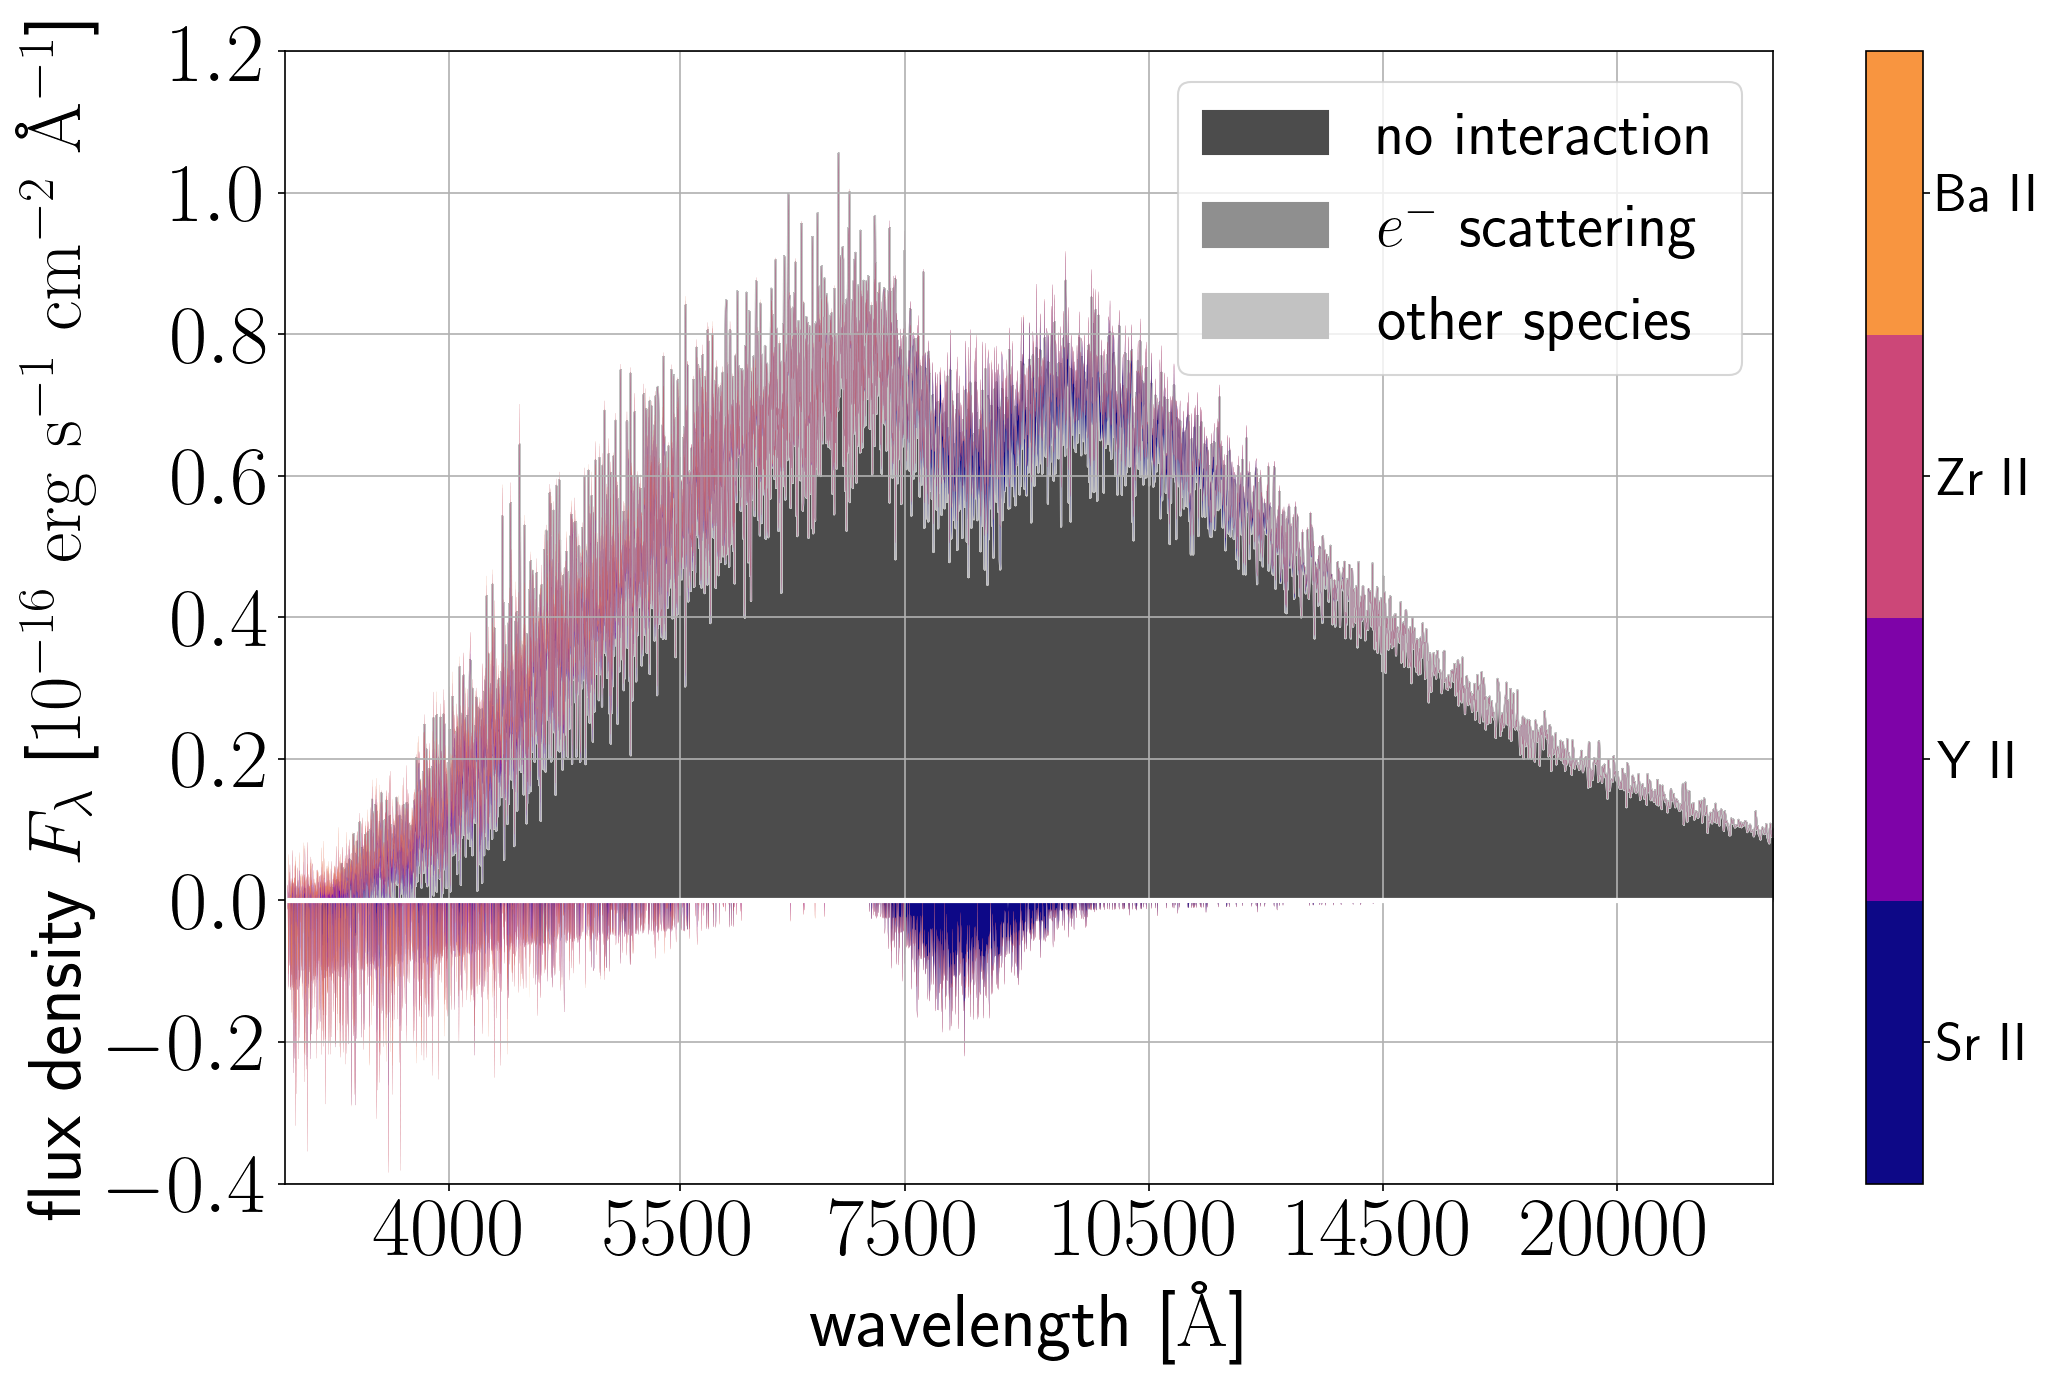
\includegraphics[width=0.47\textwidth]{figs/appendix/SDEC/221024_080947_single_TARDIS_eval_SDEC.png}
    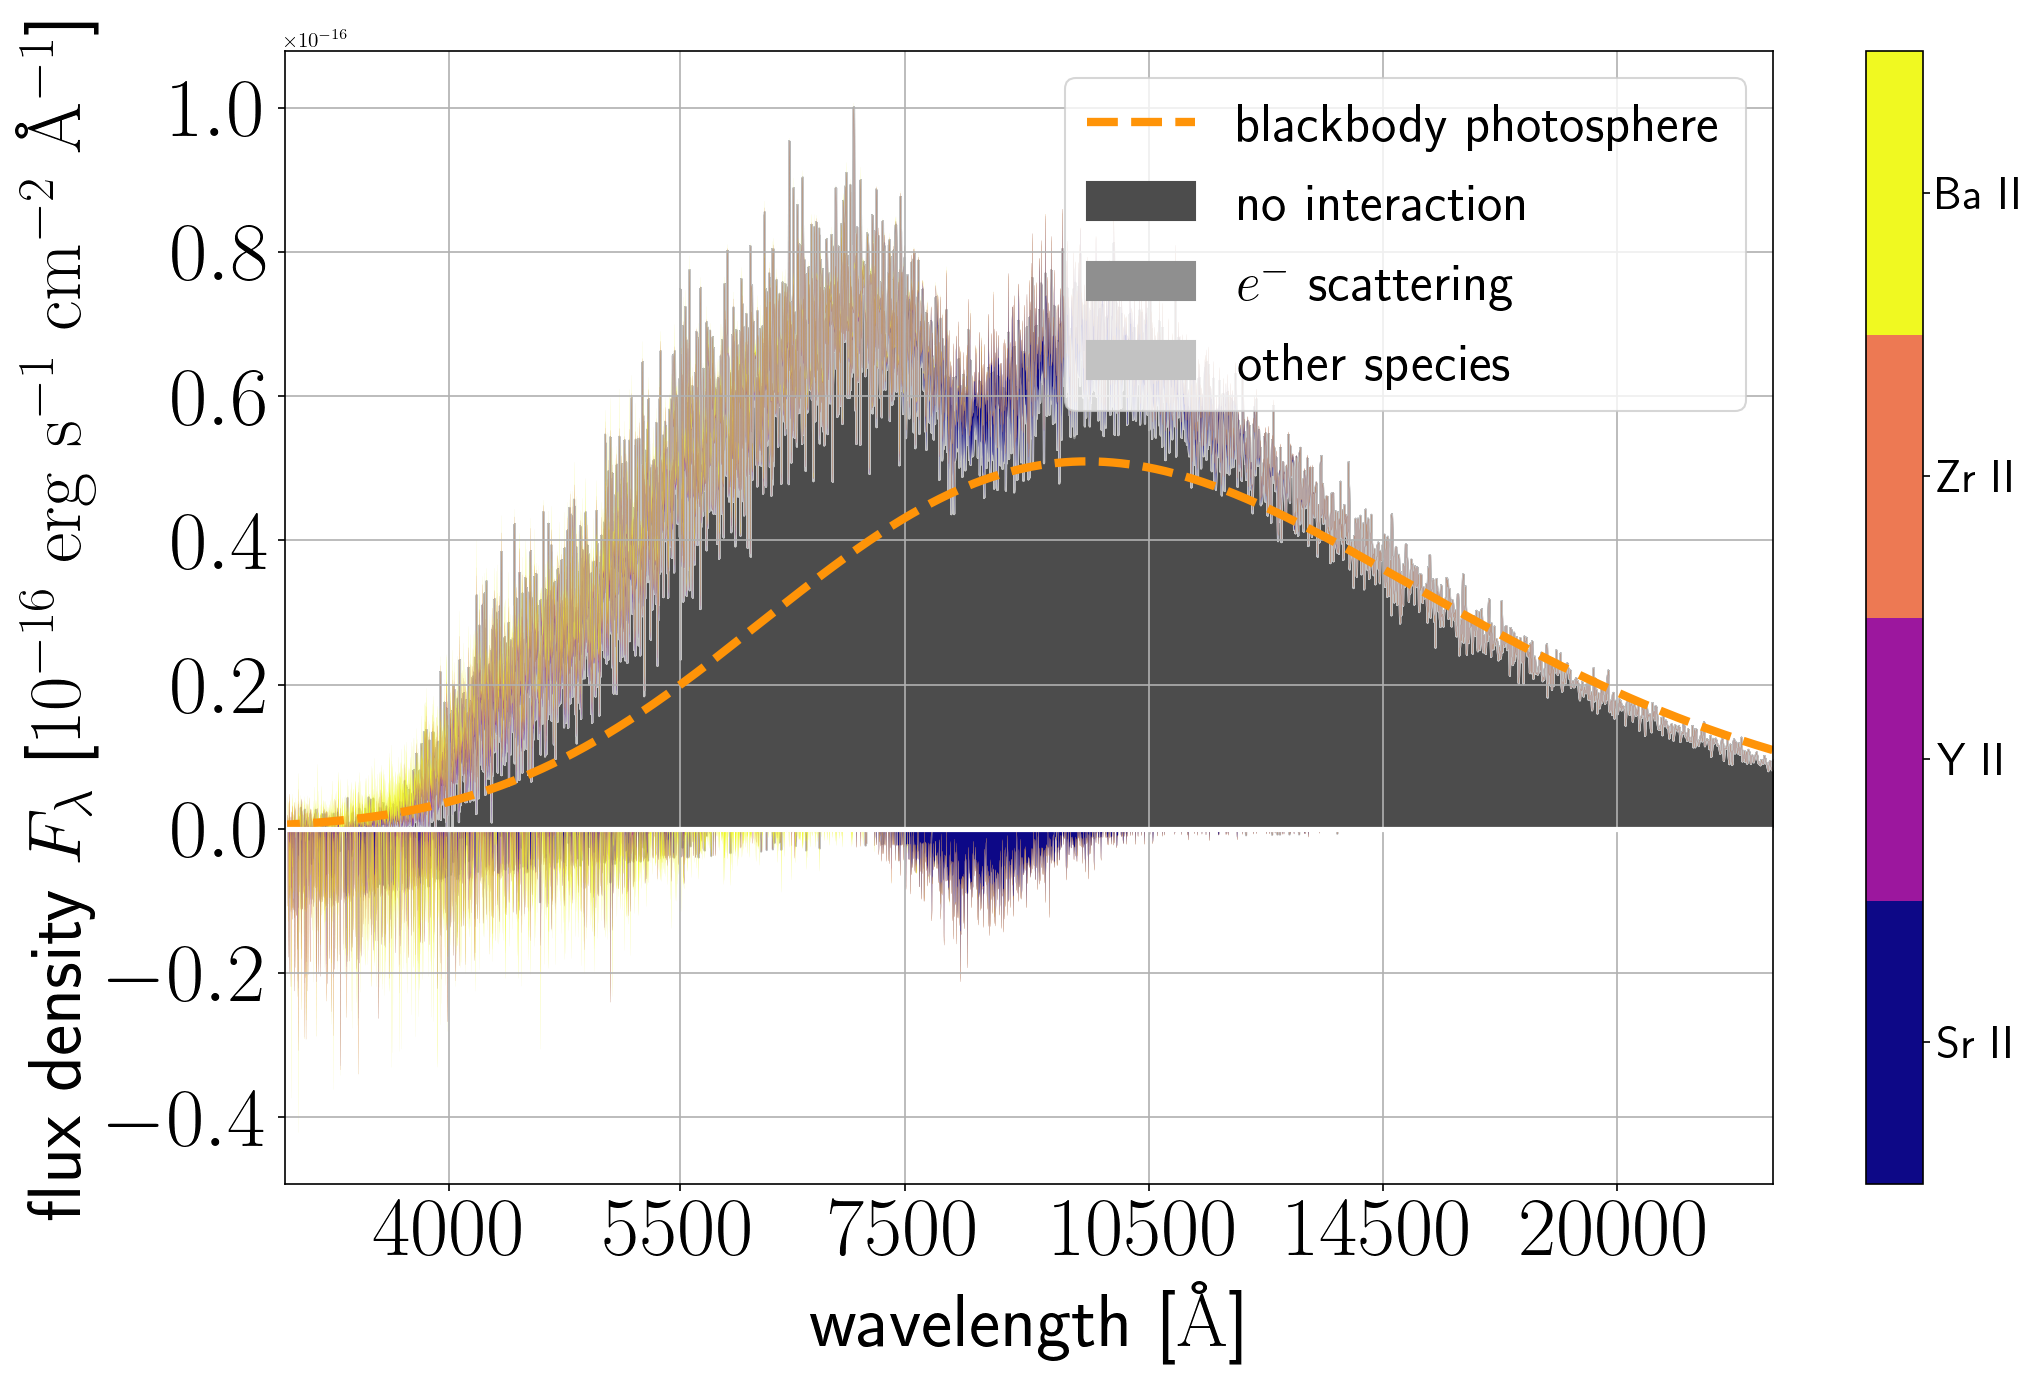
\includegraphics[width=0.47\textwidth]{figs/appendix/SDEC/230412_035244_single_TARDIS_eval_SDEC.png}
    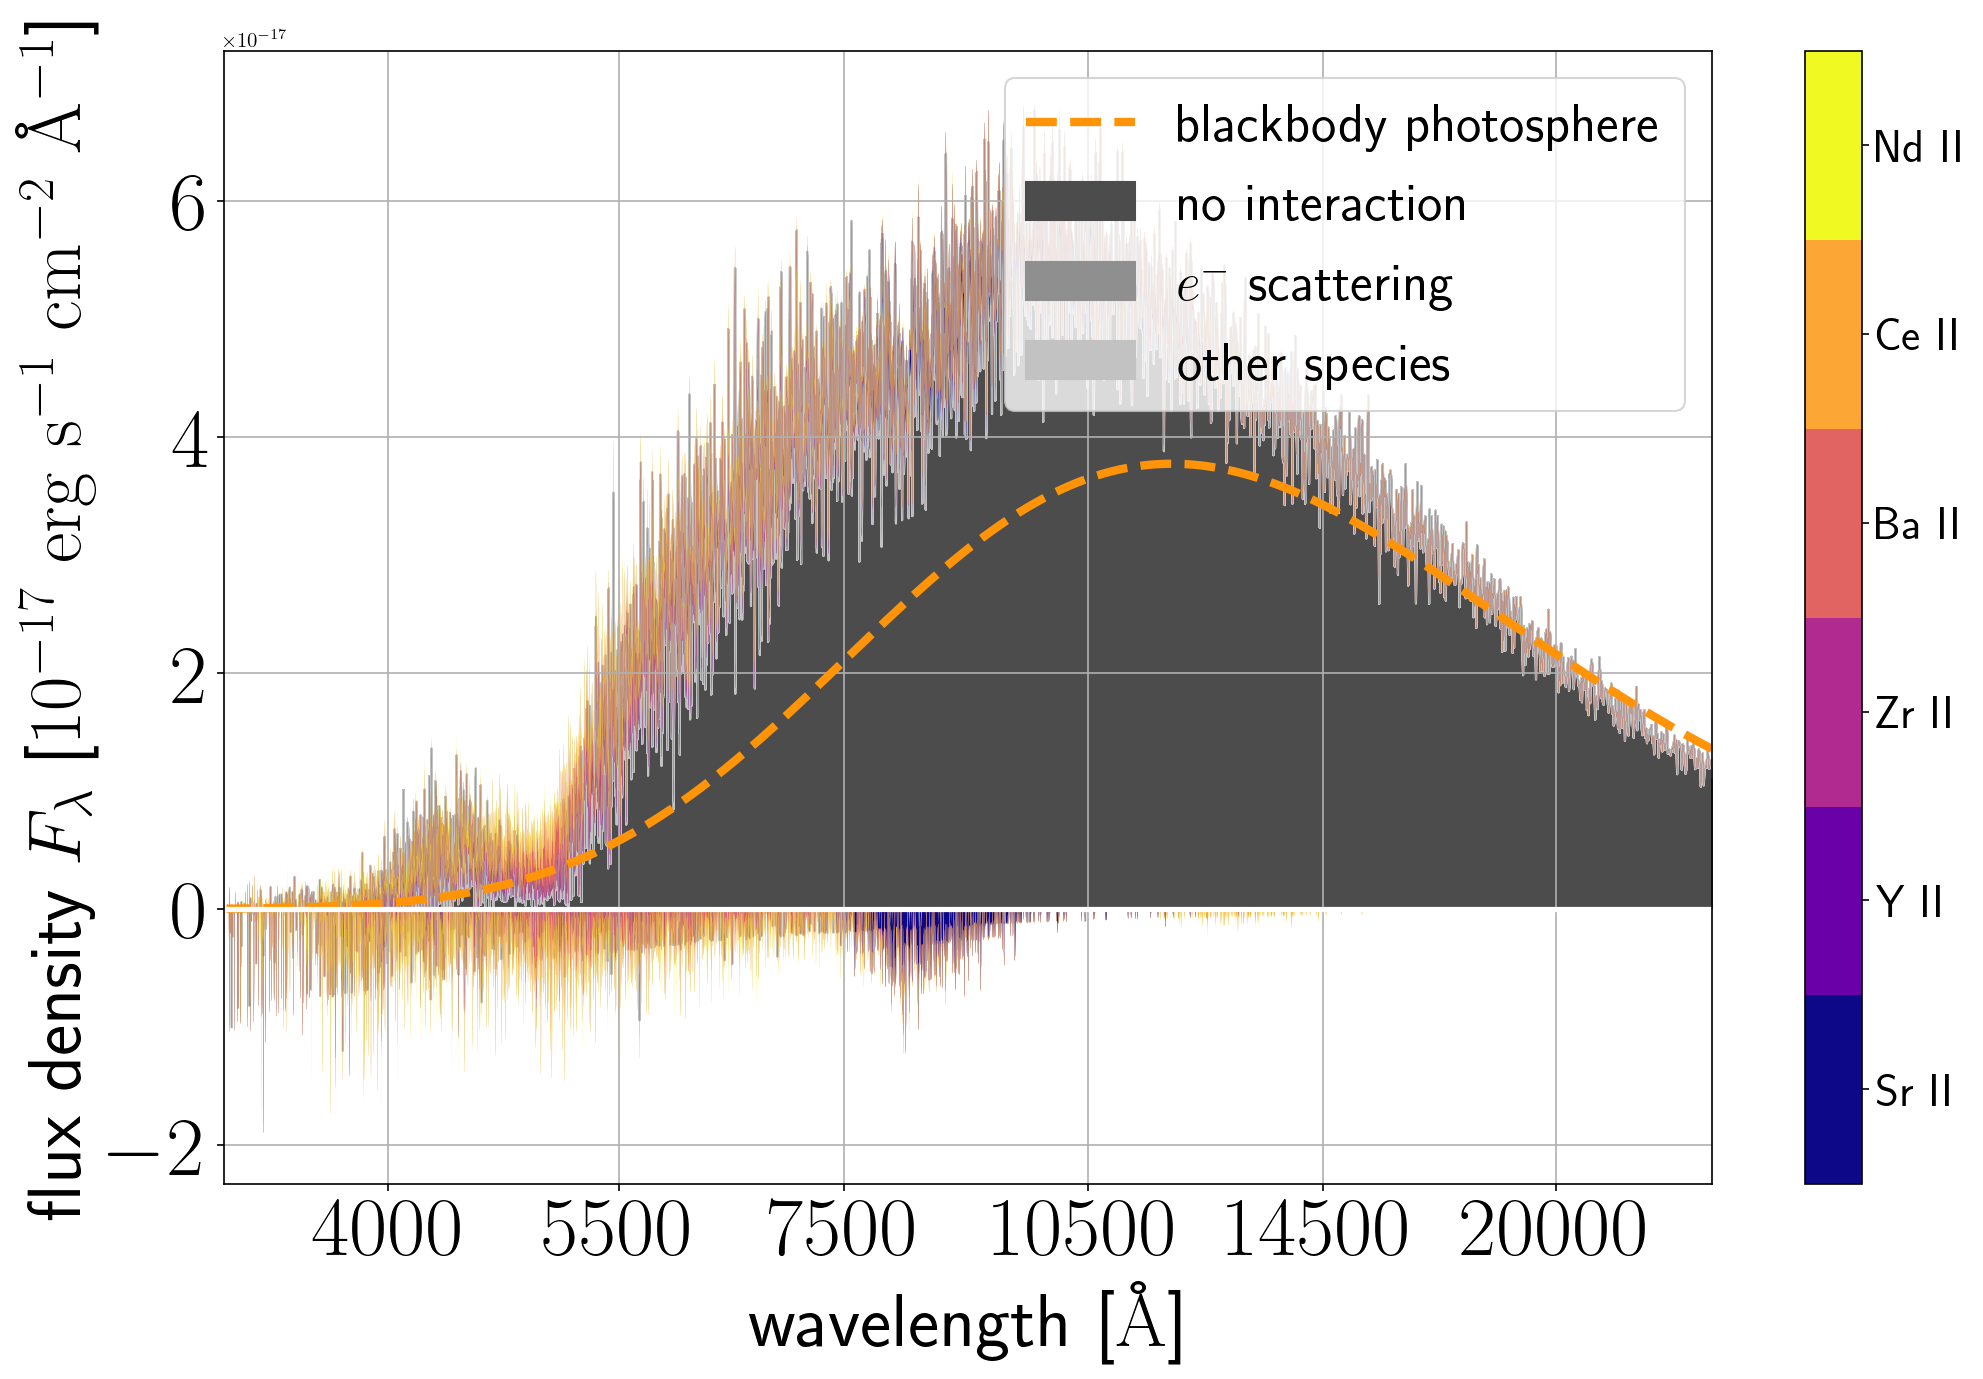
\includegraphics[width=0.47\textwidth]{figs/appendix/SDEC/230621_082134_single_TARDIS_eval_SDEC.png}
    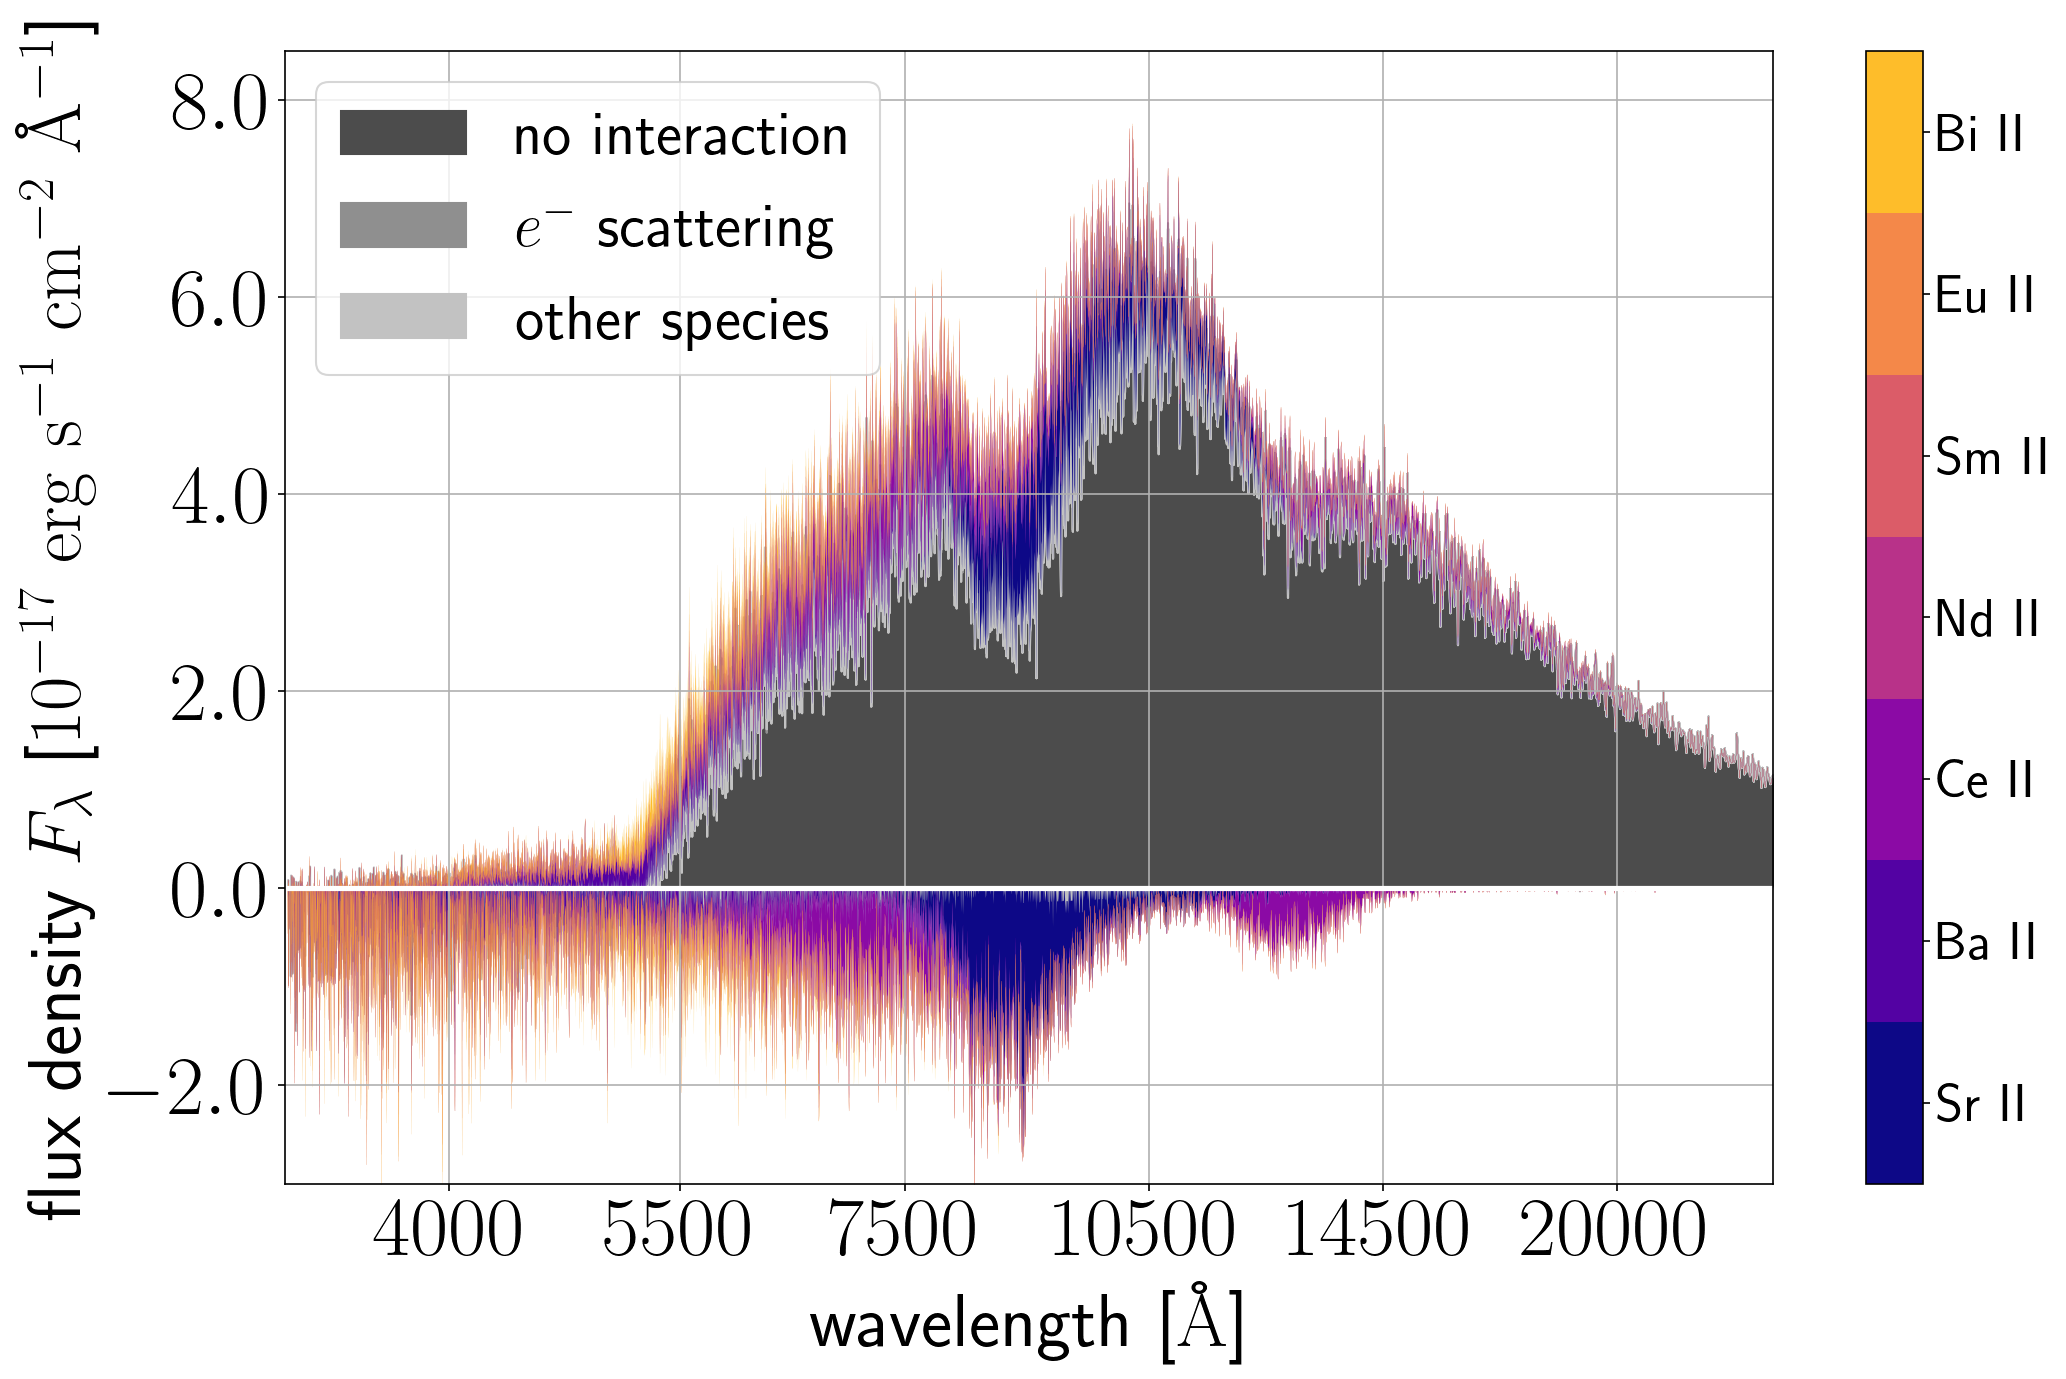
\includegraphics[width=0.47\textwidth]{figs/appendix/SDEC/230626_073230_single_TARDIS_eval_SDEC.png}
    \figcaption{\textbf{Spectral DEComposition (SDEC) plots for all best fits, at 1.4, 2.4, and 3.4 days, for single- and multi-component models}. The left column contains single-component models for 1.4, 2.4, and 3.4 days; the right contains multi-component equivalents. The ions \ion{Sr}{2}, \ion{Y}{2}, and \ion{Zr}{2} produce significant absorption in all 1.4 day and 2.4 day models. The 2.4 day models also show absorption from \ion{Ba}{2}. The 3.4 day single-component model (which is a poor fit to the observed spectrum, but nonetheless the best fit possible with a single component) exhibits absorption from all four of these ions, except \ion{Zr}{1} in the place of \ion{Zr}{2}, due to the cooler ejecta. The spectrum also shows moderate absorption from ions of three lanthanides: \ion{La}{2}, \ion{Ce}{2}, and \ion{Nd}{2}. The 3.4 multi-component model, which is favored over the single-component, shows absorption from two open $s$-shell elements in the same periodic table group (\ion{Sr}{2} and \ion{Ba}{2}), four lanthanide ions (\ion{Ce}{2}, \ion{Nd}{2}, \ion{Sm}{2}, and \ion{Eu}{2}), and one ion of an especially heavy element, \ion{Bi}{2}. Furthermore, unlike at earlier epochs, ions of Y and Zr do not dominate absorption in the 3.4 day multi-component model.}\label{fig:SDEC}
\end{figure*}



%%% === APPENDIX G === %%%
%% CONVERGENCE OF FITS %%
\section{Convergence of fits}\label{app:convergence}

We assess the convergence of all fits using two methods: (1) convergence of the posterior, as measured by the \approxposterior~$z$ convergence diagnostic, and (2) convergence of the hyperparameters of the GP surrogate for the posterior. Figure X shows both diagnostics for the 2.4 and 3.4 day single-component fits, and the 1.4, 2.4, and 3.4 day multi-component fits. In all cases, convergence is obtained, and the final posterior is stable as more active learning samples are added to the training set.


% %% double-column, each row showing convergence z and GP hyperparameters
% \begin{figure*}[!ht]
%     \centering
%     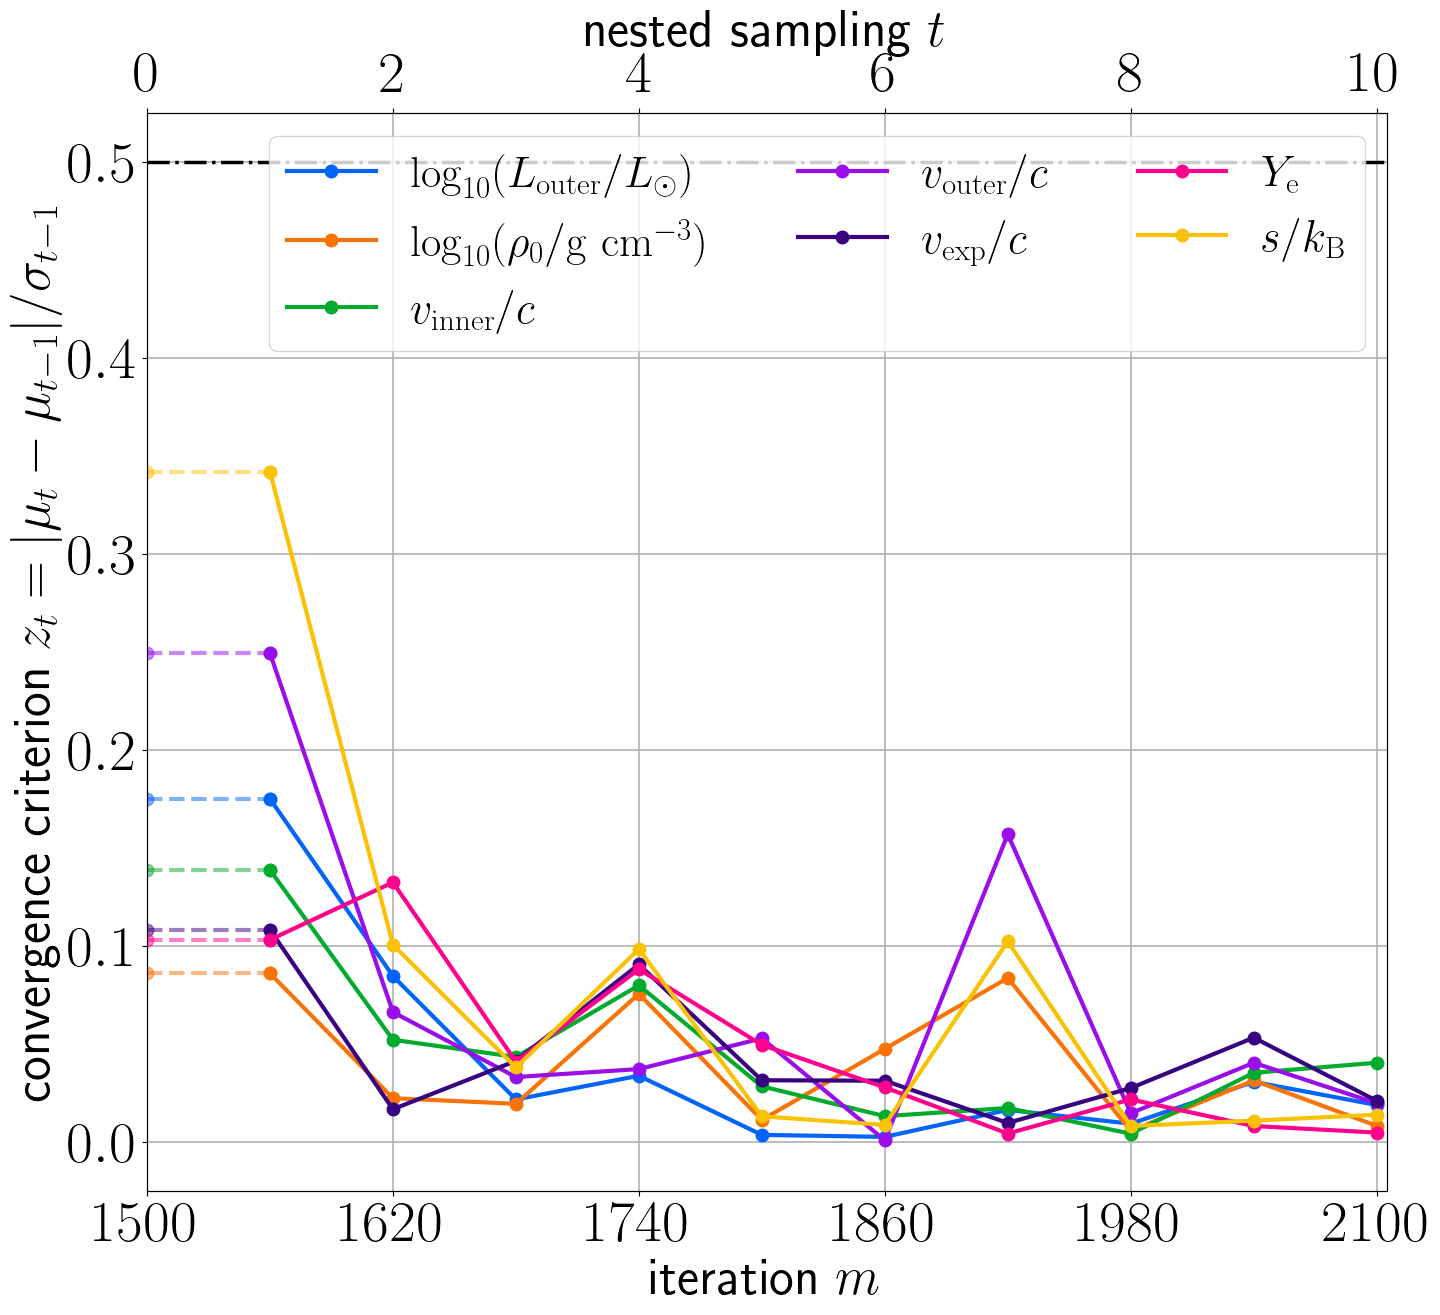
\includegraphics[width=0.2\textwidth]{figs/appendix/221022_084052_dynesty-sampling_convergence_z_eps0.5.png}
%     \includegraphics[width=0.2\textwidth]{figs/appendix/2.4d_single_GPhparams.png}
%     \\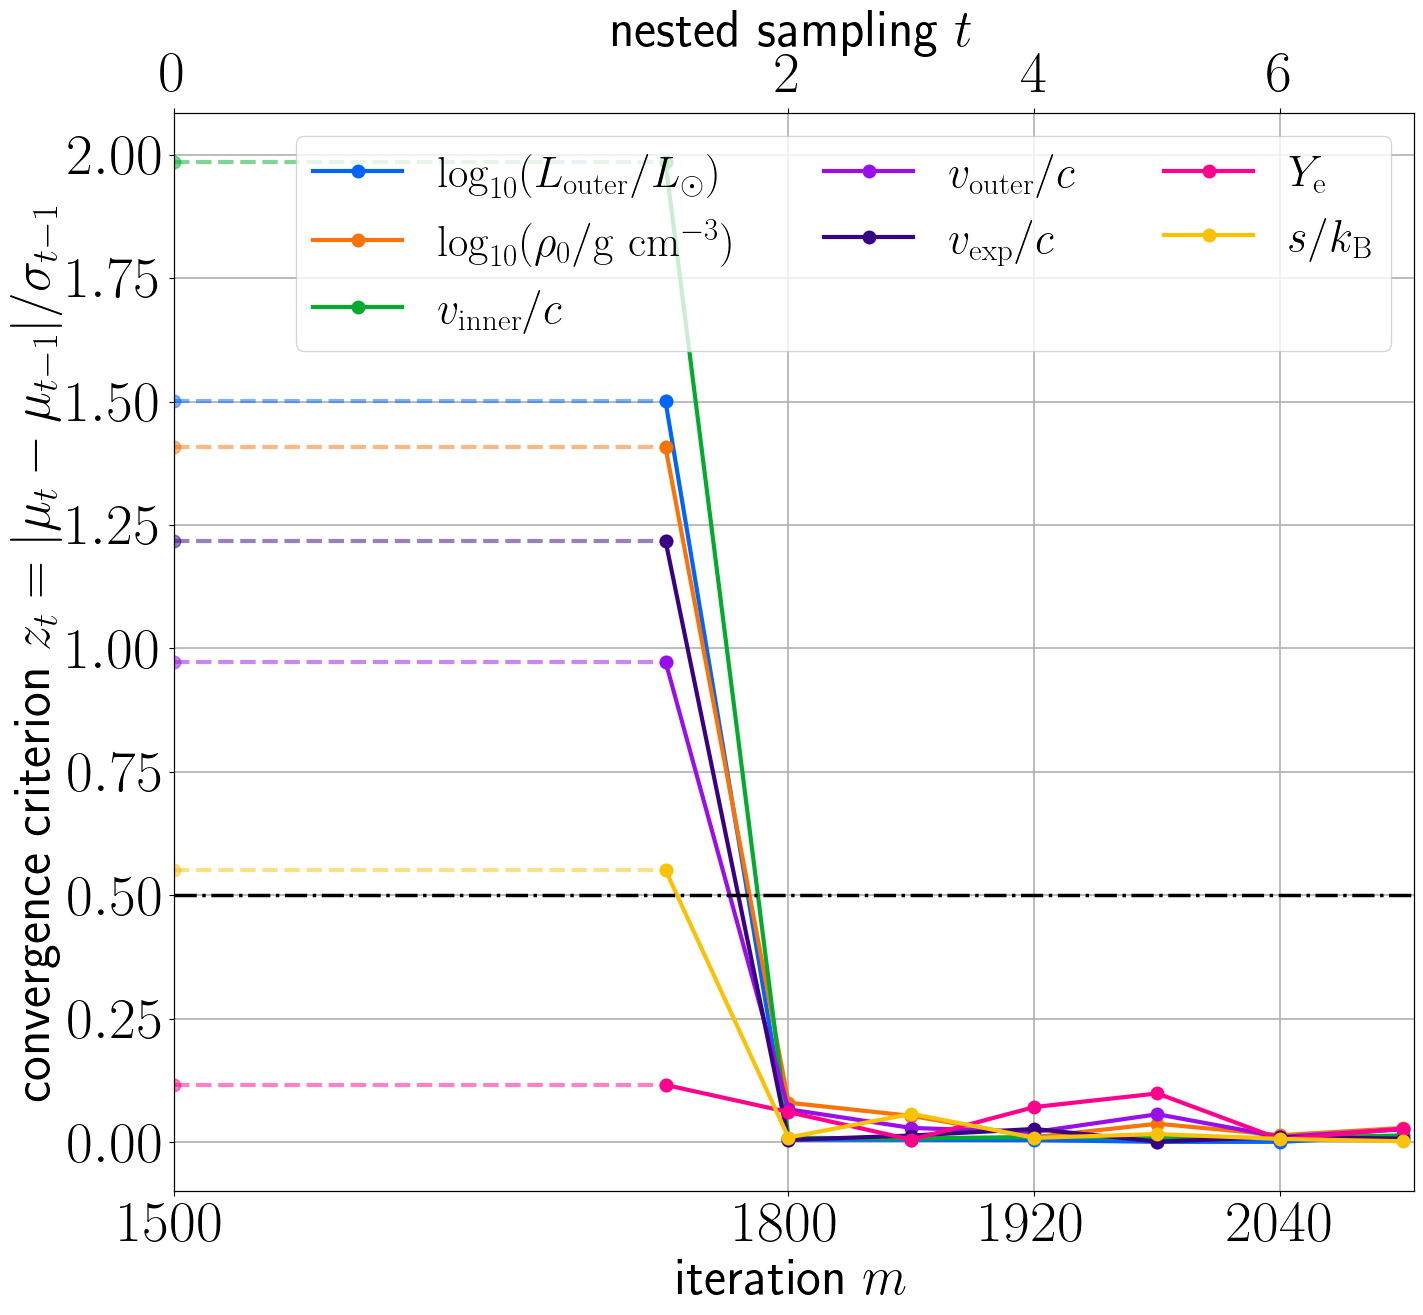
\includegraphics[width=0.2\textwidth]{figs/appendix/230618_143307_dynesty-sampling_convergence_z_eps0.5.png}
%     \includegraphics[width=0.2\textwidth]{figs/appendix/3.4d_single_GPhparams.png}
%     \\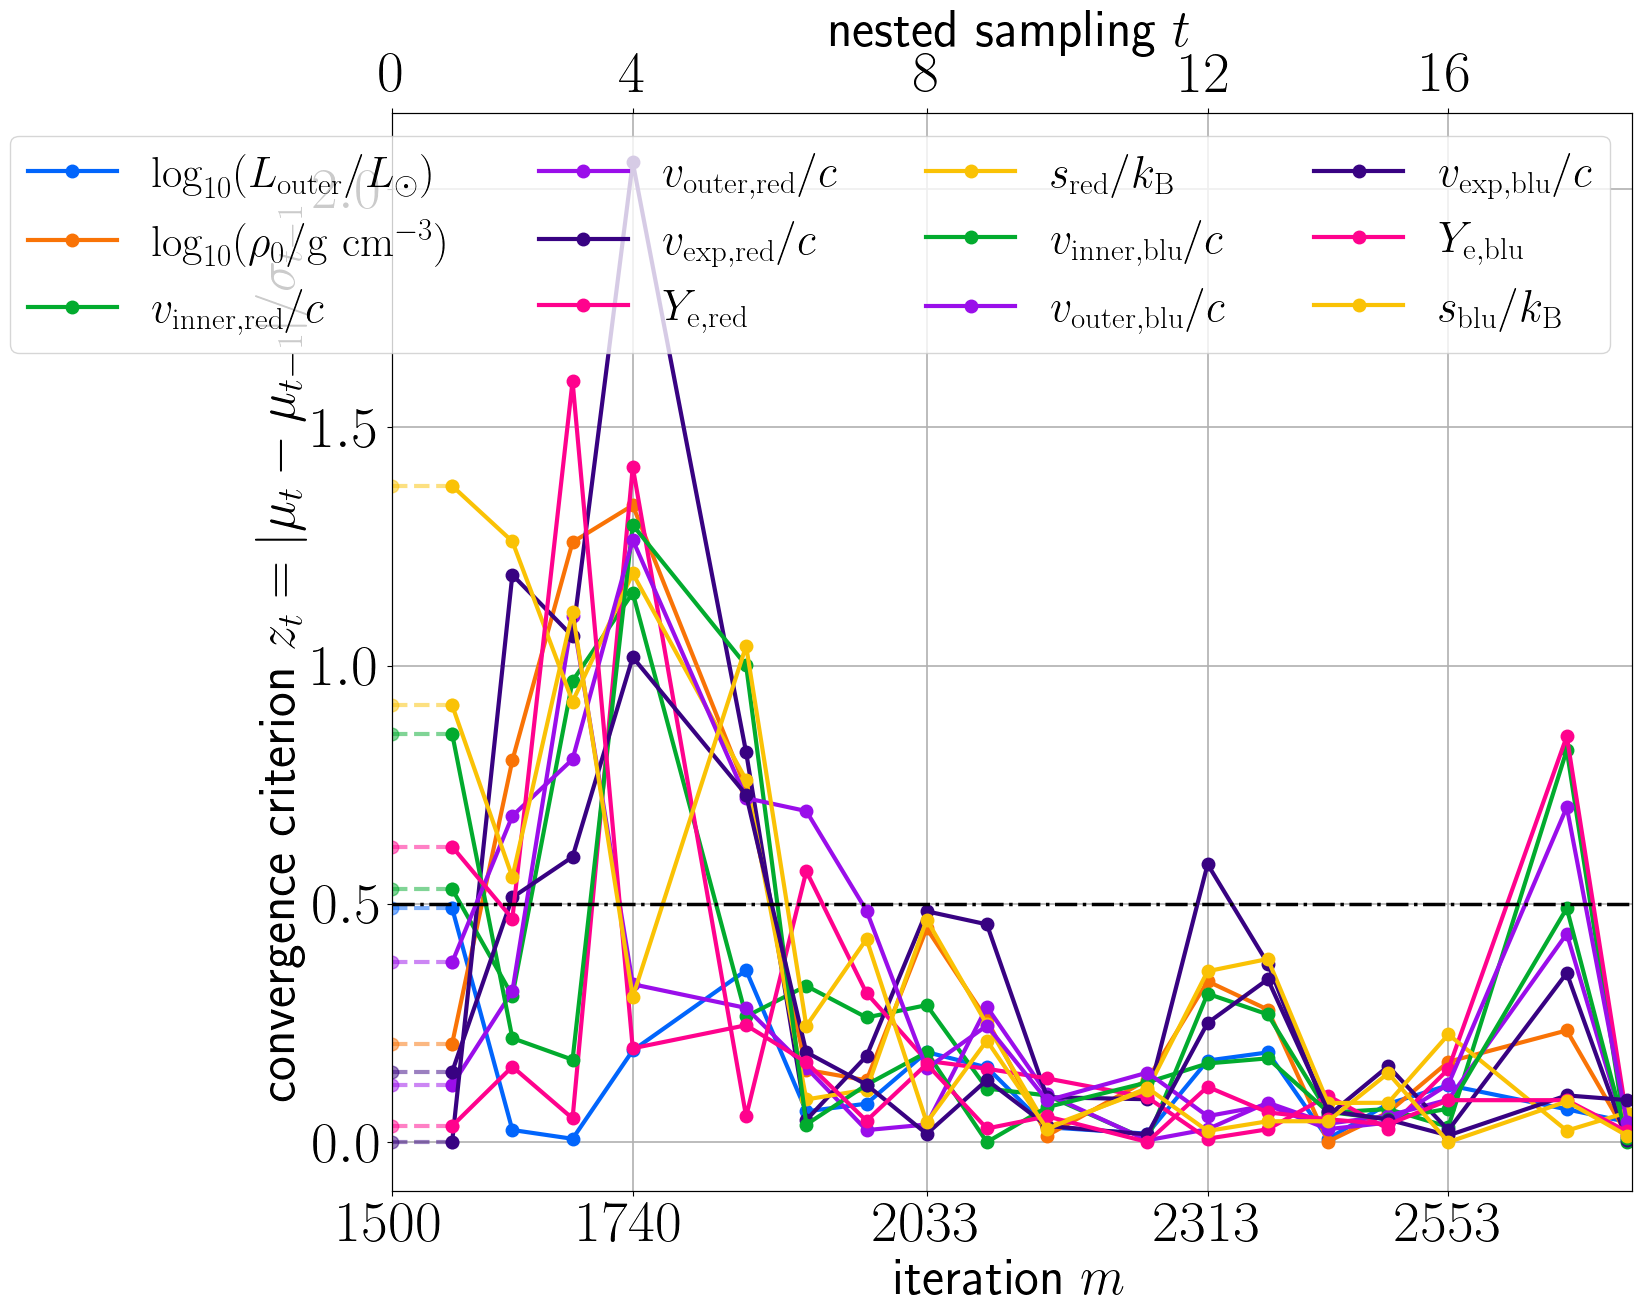
\includegraphics[width=0.2\textwidth]{figs/appendix/230103_064024_dynesty-sampling_convergence_z_eps0.5.png}
%     \includegraphics[width=0.2\textwidth]{figs/appendix/1.4d_multi_GPhparams.png}
%     \\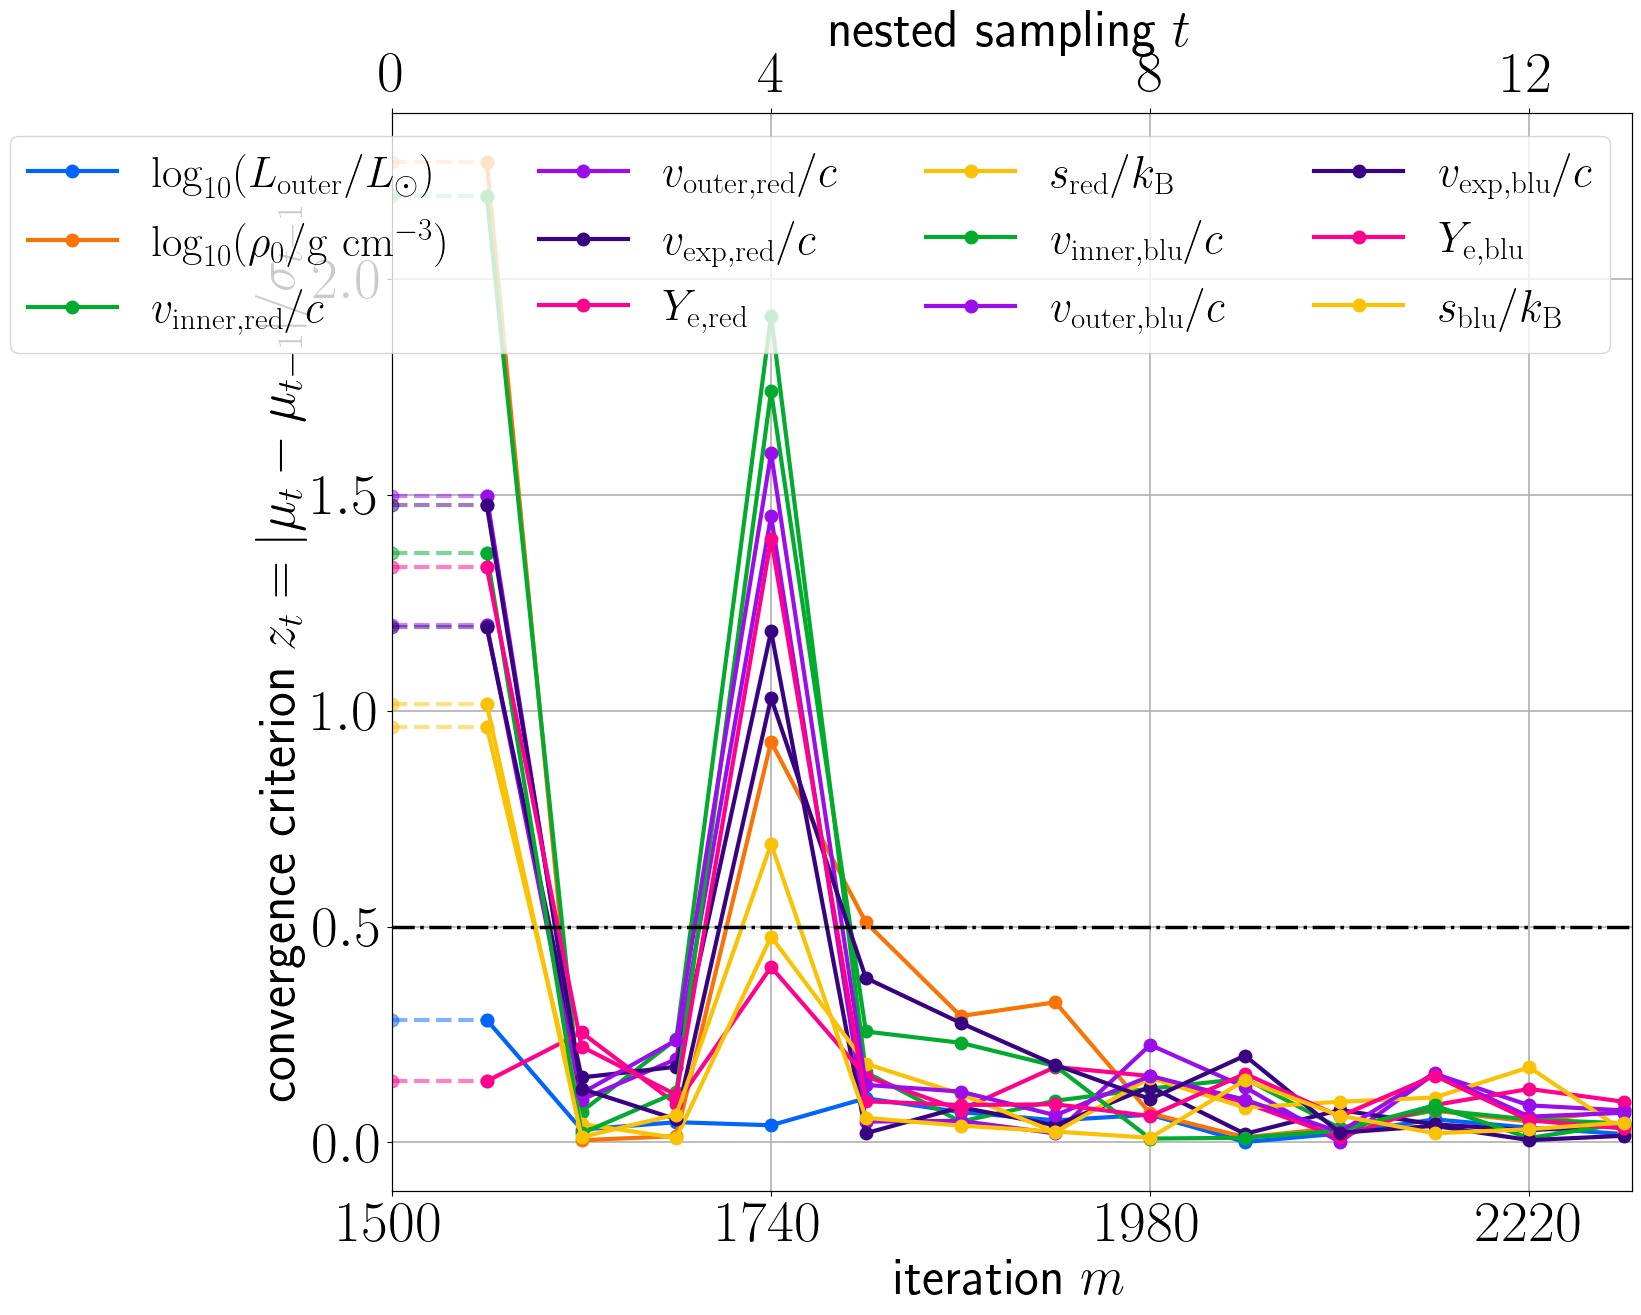
\includegraphics[width=0.2\textwidth]{figs/appendix/230103_060017_dynesty-sampling_convergence_z_eps0.5.png}
%     \includegraphics[width=0.2\textwidth]{figs/appendix/2.4d_multi_GPhparams.png}
%     \\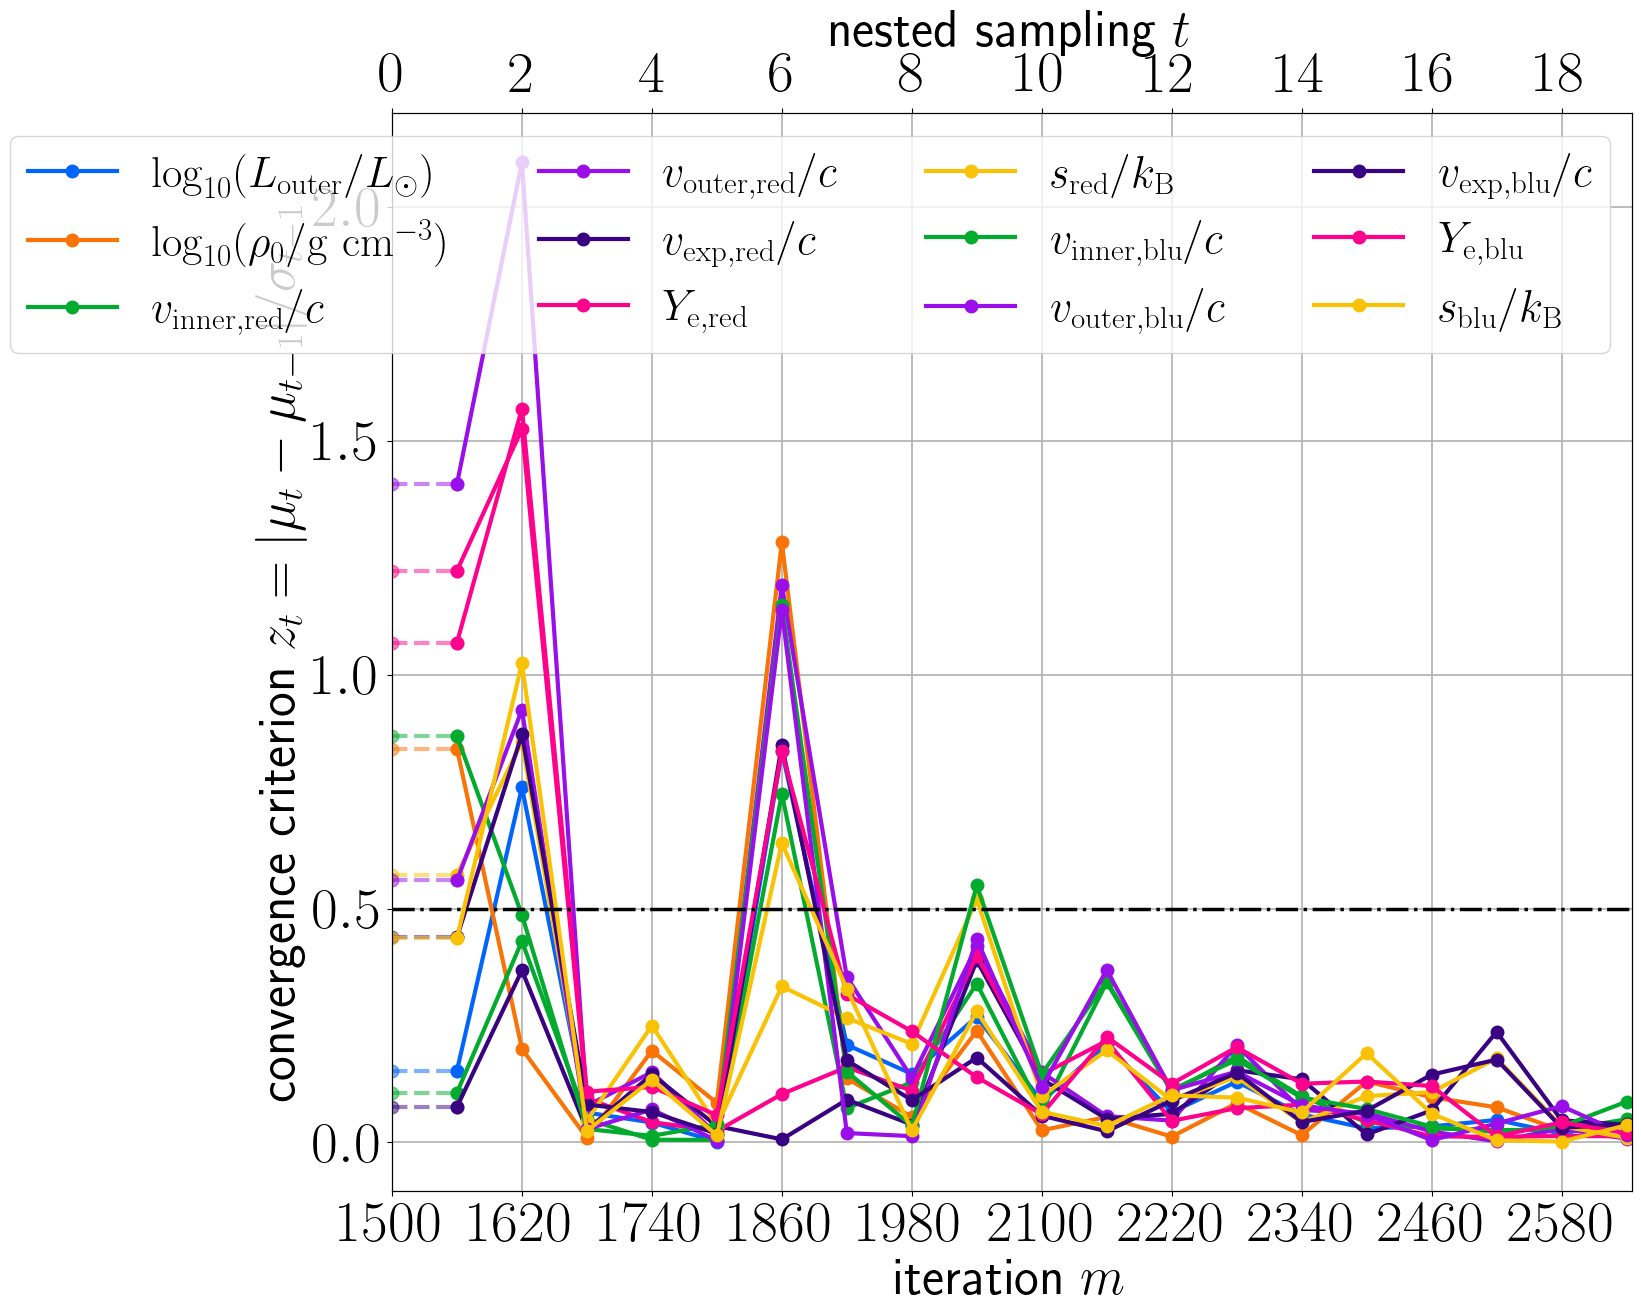
\includegraphics[width=0.2\textwidth]{figs/appendix/230622_230103_dynesty-sampling_convergence_z_eps0.5}
%     \includegraphics[width=0.2\textwidth]{figs/appendix/3.4d_multi_GPhparams.png}
%     \figcaption{Convergence of the GP, measured with the convergence diagnostic $z$ and the actual optimized hyperparameters}\label{fig:convergence}
% \end{figure*}


% ============================

\end{document}
